%--------------------
% document principal
%--------------------
% cal compilar amb `pdflatex -shell-escape main.tex`
% makeglossaries main
%--------------------
\documentclass[paper=a4,parskip=half,
twoside,fontsize=11pt,BCOR12mm,
%oneside,fontsize=11pt, %%format web
% twoside,openany,fontsize=10pt,DIV = 10,BCOR12mm, %%format en paper
]{scrbook}
%%%%BCOR12mm  factor de correcció per enquadernació
%%%%BCOR??mm  factor de correcció per enquadernació amb espiral -0.5mm??
%\usepackage[T1]{fontenc}
%------------- capçalera ----------------------
\input{capçalera.default}
\bibliography{bibliografia}
%\ExecuteBibliographyOptions{annotation=true,backref=true}
%backref=true, urldate=long, abbreviate=false,%%format web 
%---------- Mode esborrany --------------------
\includeonly
%{model}
{sgst,sgst-operacions,sgst-naturalesa}
%{sgstm,sgstm-operacions,sgstm-interpoladors,sgstm-aplicacions}
\usepackage[catalan]{todonotes} %%ús: \todo{text} \missingfigure{text}
\usepackage{fancyhdr}\pagestyle{fancyplain}\rhead{\fancyplain{--- esborrany \today\ ---}{\color{gray}{\today}}}\renewcommand{\headrulewidth}{0pt}
%\usepackage[showframe]{geometry}%page margins
%----------------------------------------------
%\usetikzlibrary{shapes,arrows,positioning}
%\usetikzlibrary{calc}
%------------- format -------------------------
%%ús coma decimal sense espais:  2{,}5
%per tal que trenqui la coma en math inline mode 
%http://tex.stackexchange.com/questions/19094/allowing-line-break-at-in-inline-math-mode-breaks-citations/
\AtBeginDocument{%
  \mathchardef\mathcomma\mathcode`\,
  \mathcode`\,="8000 
}
{\catcode`,=\active
  \gdef,{\mathcomma\discretionary{}{}{}}
}
%teoremes
\theoremstyle{plain}
\newtheorem{definition}{Definició}
\theoremstyle{definition}
\newtheorem{example}{Exemple}
\def\figureautorefname{figura} %ús: \autoref{}
\def\tableautorefname{taula} %ús: \autoref{}
\def\definitionautorefname{definició} %ús: \autoref{}
\def\exampleautorefname{exemple} %ús: \autoref{}
\def\sectionautorefname{secció} %ús: \autoref{}
%numeracions d'equacions, definicions, etc.
\numberwithin{equation}{chapter}
\numberwithin{definition}{chapter}
\numberwithin{example}{chapter}
%SGST-set
\DeclareMathOperator*{\inst}{\in^t}
\DeclareMathOperator*{\notinst}{\notin^t}
\DeclareMathOperator*{\cupt}{\cup^t}
\DeclareMathOperator*{\dift}{-^t}
\DeclareMathOperator*{\capt}{\cap^t}
\DeclareMathOperator*{\where}{where}
\DeclareMathOperator*{\rename}{rename}
\DeclareMathOperator*{\as}{as}
\DeclareMathOperator*{\join}{join}
\DeclareMathOperator*{\semijoin}{semijoin}
\DeclareMathOperator*{\map}{mapa}%mapa (map), aplica 
\DeclareMathOperator*{\agg}{agregat}%agregat (aggregate)
\DeclareMathOperator*{\fold}{plec}%plec (fold)
%SGST-seq
\DeclareMathOperator*{\seg}{seg}
\DeclareMathOperator*{\ant}{ant}




\newcommand{\R}{\mathbb{R}} % the set of real numbers
\newcommand{\N}{\mathbb{N}}
%\newcommand{\acro}[1]{\textsc{\lowercase{#1}}}

\usepackage{longtable}
\usepackage{subcaption}
\usepackage{multirow}
\usepackage{pgfplots}
\usetikzlibrary{dateplot}
\usetikzlibrary{shapes,arrows,positioning}
%\usetikzlibrary{dateplot}  
%\usetikzlibrary{pgfplots.groupplots}






% \pgfplotsset{
%    rrbtimeseries/.style={
%         % date coordinates in=x,
%         ylabel=Temperature (K),
%         % legend style={font=\footnotesize},
%         % tick label style={font=\footnotesize},
%         % every axis x label/.style={
%         %   at={(1.3,0)},
%         %   anchor=north,
%         %   },
%         % label style={font=\footnotesize},
%         % xticklabel style= {rotate=17,anchor=north east},
% %        every axis title shift=0pt,
% %        max space between ticks=15,
%        %  every mark/.append style={mark size=6},
%        %  major tick length=0.1cm,
%        %  minor tick length=0.066cm,
%        %  very thin,
%        %  every axis legend/.append style={
%        %    at={(1.2,0)},
%        %    anchor=south east,
%        %    draw = none},
%        % legend columns = 4,
%        % unbounded coords=jump, %v>1.4
%     },

%   % rrbrs/.style={
%   %       rrbtimeseries,
%   %       width = \textwidth,
%   %       height = 0.25\textwidth,
%   %       every axis x label/.style={
%   %         at={(1.3,-1)},
%   %         anchor=north,
%   %         },
%   %       ylabel = {},  
%   %       max space between ticks=50,
%   %       every axis legend/.append style={
%   %         at={(1,-1.1)},
%   %         anchor=north east,
%   %         draw = none},
%   %       title style={font=\small,below,anchor=north,fill=white},
%   %   },
%  }




\pgfplotsset{
   timeseries/.style={
        date coordinates in=x,
        ylabel=Temperature (K),
        legend style={font=\footnotesize},
        tick label style={font=\footnotesize},
        every axis x label/.style={
          at={(1.3,0)},
          anchor=north,
          },
        label style={font=\footnotesize},
        xticklabel style= {rotate=17,anchor=north east},
%        every axis title shift=0pt,
%        max space between ticks=15,
        every mark/.append style={mark size=6},
        major tick length=0.1cm,
        minor tick length=0.066cm,
        very thin,
        every axis legend/.append style={
          at={(1.2,0)},
          anchor=south east,
          draw = none},
       legend columns = 4,
    },
    rd/.style={
        timeseries,
        every axis x label/.style={
          at={(1.3,-1)},
          anchor=north,
          },
        label style={font=\footnotesize},
        ylabel = {},
        width=17cm,
        height=3.5cm,   
        max space between ticks=50,
        every axis legend/.append style={
          at={(1,-1.1)},
          anchor=north east,
          draw = none},
        title style={font=\small,below, at={(0.7,1.7)},anchor=north,fill=white},
    }
}


%        unbounded coords=jump, %v>1.4
%        unbounded coords=discard, %v>1.4


%http://tex.stackexchange.com/questions/46422/axis-break-in-pgfplots

%http://tex.stackexchange.com/questions/52409/insert-a-separate-mark-inside-a-pgfplots-graph


%glossaris
\usepackage[
          acronym,
          %%nonumberlist,
          %%toc,
          section,
          numberedsection=autolabel,
          sanitize=none, %pels accents en el vegeu
          ]{glossaries}
%\renewcommand*{\glspostdescription}{}%anul·la el punt final
\renewcommand*{\acronymname}{Sigles}%{Índex de sigles}??si té refs pàgines 
%Índex d'abreviacions?? si conté abreviatures o símbols
% \short<type>name,
\newglossary{notation}{not}{ntn}{Notació}
\newglossarystyle{estil-notation}{%
  \renewcommand{\glsgroupskip}{}% make nothing happen between groups
  \renewenvironment{theglossary}
  {\begin{longtable}{lll}
      % \caption{Notació dels SGSTM \label{tab:sgstm-simbols}}
      % \endfirsthead
      % \caption[]{Notació dels SGSTM (continuació)}
      % \endhead
          % \endfoot
          % \endlastfoot
    }{\end{longtable}}
  \renewcommand*{\glossarysubentryfield}[6]{%
    %\glstarget{##2}{##3}% the entry name
    \glstarget{##2}{\Glsentryname{##2}}% the entry name
    &
     %\space (##5)% the symbol in brackets
    \space ##4% the description
    &
    \space [##6]% the number list in square brackets
    \\
  }%
  \renewcommand*{\glossaryentryfield}[5]{%
    \\\pagebreak[3]\hline
    \glossarysubentryfield{##2}{##1}{##2}{##3}{##4}{##5}
    \hline
  }
}


\renewcommand{\seename}{vegeu}
\renewcommand{\entryname}{Notació}
\renewcommand{\descriptionname}{Descripció}

\makeglossaries


%\renewcommand{\glossarypreamble}{Text com a préambul}



%TERMES


%temps real
\newglossaryentry{TempsReal}{name={temps real}, description={(\emph{real time}), sistemes que han de respondre amb un temps determinat. A vegades també s'utilitza el terme com a adjectiu per a designar sincronització real amb el rellotge o per a indicar que l'usuari no percep retards. Allà on pugui causar confusió, utilitzarem sincronitzat o en línia (\emph{online}) per al segon significat.}
}





\newglossaryentry{SistemaGestioBaseDades}{name={sistema de gesti{ó} de base de dades}, description={(\emph{Data Base Management System})} }




%terme:SGBDR

\newglossaryentry{terme:SGBDR}{name={sistema de gestió de base de dades relacional}, description={(\emph{Relational Data Base Management System}). 
També anomenat 'object/relational' DBMS \parencite{date06}.
Totes les definicions són coherents amb \textcite{date:introduction} } }



%model, implementació
%Els SGBD es basen en teories matemàtiques que reben el nom de model de dades, un SGBD és una implementació d'un model de dades.
%Segons \citeauthor{date:introduction}, ``un model de dades és una definició abstracta, auto continguda i lògica dels objectes, de les operacions i  de la resta que conjuntament constitueixen la màquina abstracta amb la que els usuaris interactuen. Els objectes permeten modelar l'estructura de les dades. Les operacions permeten modelar el comportament''. Ara bé, \citeauthor{date:introduction} avisa que el concepte model de dades també s'usa per a definir una estructura persistent de dades concreta i per tant cal distingir adequadament la confusió entre els dos conceptes.
% Tal com fa Date, parlarem de model de dades en el primer sentit de màquina abstracta i a vegades ho abreviarem com a model.


%tipus,valor,variable,operador

\newglossaryentry{terme:SGBDR:domini}{see={terme:SGBDR},name={domini}, description = {(\emph{domain}), equivalent a tipus de dades.
Conjunt de valors. Cada domini té associat un conjunt d'operadors, en alguns casos fins i tot s'entén que el domini inclou els operadors (concepte de classe a orientació a objecte). Els tipus tenen una representació (estructura) o més d'una, és a dir els seus valors poden estar denotats per més d'un literal} }
\newglossaryentry{terme:SGBDR:tipus}{see={terme:SGBDR:domini}, name={tipus de dades}, description = {(\emph{data type}), a vegades solament 'tipus' (\emph{type}) o bé 'tipus de dades abstracte' (\emph{abstract data type}). Segons \textcite{date:introduction} en el context de model tots els tipus de dades han de ser abstractes} }

\newglossaryentry{terme:SGBDR:escalar}{parent={terme:SGBDR:domini}, name={escalar}, description = {Un tipus és escalar (\emph{scalar}) quan no té components visibles a l'usuari i és no escalar (\emph{nonscalar}) en cas contrari; no obstant, tant els escalars com els no escalars tenen representació, la qual pot contenir components} }


\newglossaryentry{terme:SGBDR:valor}{see={terme:SGBDR},name={valor}, description = {(\emph{value}), equivalent a objecte i instància.
'Constant individual' que és d'un tipus de dades. A vegades s'utilitza 'constant' per designar una  variable que mai canvia de valor, però aquest no és el cas d'aquesta definició} }
\newglossaryentry{terme:SGBDR:objecte}{see={terme:SGBDR:valor}, name={objecte}, description = {(\emph{object})} }
\newglossaryentry{terme:SGBDR:instancia}{see={terme:SGBDR:valor}, name={instància}, description = {(\emph{instance})} }

\newglossaryentry{terme:SGBDR:literal}{see={terme:SGBDR},name={literal}, description = {(\emph{literal}).
Símbol que denota un valor. Un valor pot estar denotat per més d'un literal. Segons aquesta definició literal no és equivalent a valor} }


\newglossaryentry{terme:SGBDR:variable}{see={terme:SGBDR},name={variable}, description = {(\emph{variable}).
Contenidor d'una aparició d'un valor. El valor que conté la variable pot ser canviat mitjançant l'operador d'assignació. En canvi els valors, per si mateixos, no poden ser actualitzats} } %A l'esquerra de l'operador d'assignació sempre hi ha variables, tot i que s'admeten simplificacions mitjançant expressions que són pseudovariables (p.ex. s[1] := 3 és equivalent a s := [s[0],3,s[2],..]).
%Les variables tenen adreces (\emph{addresses}) i per tant es pot apuntar (\emph{point to}) a les variables mitjançant els operadors de referència (\emph{referencing}), el qual retorna l'adreça d'una variable, i de desreferència (\emph{dereferencing}), el qual retorna la variable a partir de l'adreça. Els valors adreces pertanyen al tipus apuntador, però el model relacional prohibeix els valors de tipus apuntador i per tant no té REF ni DEREF; les relvar s'identifiquen pel seu nom i no cal que tinguin adreça. (Compte que en orientació a objectes una variable és el contenidor d'un valor que és un ID d'objecte, és a dir és el contenidor d'una referència).



%relació
\newglossaryentry{terme:SGBDR:relacio}{%
  see={terme:SGBDR},%
  name={relació},%
  plural={relacions},%
  sort={relacio},%
  description = {(\emph{relation}). Pot referir-se tant a tipus,
    valor, literal o variable relació. És l'objecte principal d'estudi
    en els SGBDR i de manera popular s'anomena taula. \emph{Nota}:
    hi ha certes diferències lògiques entre les relacions del model
    relacional i les relacions tal com es defineixen en matemàtiques.
  }%
}










%terme:tipus

% %reals projectius
% \newglossaryentry{terme:tipus:real-projectiu}{%
%   see={terme:SGBDR:tipus},%
%   name={real projectiu},%
%   plural={reals projectius},%
%   symbol={\ensuremath{\bar\mathbb{R}}},%
%   description = {(\emph{projective extended real
%       numbers}). 
% %$\bar\mathbb{R}\in\mathbb{R}\cup$
% %\{-\infty,+\infty\}$.
%   }%
% }





% [date2005]
% The original version of the model also omitted a few things I now consider vital. For example, it excluded any
% mention—at least, any explicit mention—of all of the following: predicates, constraints (other than candidate
% and foreign key constraints), relation variables, relational comparisons, relation type inference and associated
% features, certain algebraic operators (especially rename, extend, summarize, semijoin, and semidifference),
% and the important relations TABLE_DUM and TABLE_DEE.




%pendent: falta posar el name

% \newglossaryentry{SGBD-model}{ description = {Un model és}, name={Model de SGBD} }



% \newglossaryentry{SBDR-cap}{ description = {La capçalera d'un SGBDR}, name={Capçalera}, parent={SGBD-model} }



% \newglossaryentry{heading}{ description = {Equivalent to intension and relation schema} }
% \newglossaryentry{intension}{ description = {}, see=heading }
% \newglossaryentry{relation schema}{ description = {}, see=heading }

% \newglossaryentry{body}{ description = {Equivalent to extension} }
% \newglossaryentry{extension}{ description = {buit}, see=body}


% \newglossaryentry{DBMS data model}{ description = {A data model (first sense) is an abstract, self-contained, logical definition of the
% objects, operators, and so forth, that together constitute the abstract machine with which
% users interact. The objects allow us to model the structure of data. The operators allow us
% to model its behavior.\cite{date}. Sometimes it is referred as architecture.
% } }

% \newglossaryentry{data model}{ description = { A data model (second sense) is a model of the persistent data of some particular
% enterprise. [date06]. }}


% \newglossaryentry{DBMS implementation}{ description = {An implementation of a given data model is a physical realization on a real
% machine of the components of the abstract machine that together constitute that model.\cite{date}} }


% \newglossaryentry{data independence}{ description = {model and implementation kept separated}}




% \newglossaryentry{relationships}{
% description={relationships are semantic. relationships are entities.}}








%%% Local Variables: 
%%% mode: latex
%%% TeX-master: "../main"
%%% End: 

\loadglsentries{vocabulari/abreviacions.tex}
\loadglsentries[notation]{vocabulari/notacio.tex}
\newcommand{\glssymboldef}{\glssymbol[format=hyperbf,counter=definition]}
\newcommand{\glsdispdef}{\glsdisp[format=hyperbf,counter=definition]}
\newcommand{\hyperbfsec}[1]{\textbf{\S\hypersf{#1}}}
\newcommand{\glsdispsec}{\glsdisp[format=hyperbfsec,counter=subsection]}
\newcommand{\glssymbolsec}{\glssymbol[format=hyperbfsec,counter=subsection]}



%-------------- dades --------------------------
\hypersetup{
    pdftitle={Disseny i modelització d'un sistema de gestió multiresolució per a sèries temporals},
    pdfauthor={Aleix Llusà Serra},
    pdfcreator={DiPSE--UPC},
    pdfsubject={Tesi 2011--2014},
    pdfkeywords={sèries temporals; model de dades; sistemes de bases de dades; sistemes de monitoratge},
    pdflang={ca},
}

\title{Disseny i modelització d'un sistema de gestió multiresolució per a sèries temporals}
\author{Aleix Llusà Serra}
%----------------------------------------------


\begin{document}


%------------- Pàgina de títol ------------
%\maketitle
%%------------- pàgina de portada -----------
\begin{titlepage}
  \begin{center} 

   

    {\Large \scshape Universitat Politècnica de Catalunya} \vskip 1cm 

    {Programa de Doctorat:} \vskip 0.5cm 
    
    {\scshape Automàtica, Robòtica i Visió} \vfill%\vskip 4cm 

    {Tesi Doctoral} \vskip 1cm 
    
    {\scshape \bfseries \Large Disseny i modelització d'un sistema de gestió\\
 multiresolució per a sèries temporals} \vskip 2cm

    {\bfseries Aleix Llusà Serra} \vfill%\vskip 4cm 

    {Direcció:}
       
    {Teresa Escobet Canal i
    Sebastià Vila-Marta}  \vskip 1cm 
    %\vfill 

    {Juny de 2015}

\end{center}
\end{titlepage}


%------------- pàgina de crèdits -----------
{
  \thispagestyle{empty}

  \mbox{}

  \vfill

  Primera edició: setembre de 2015. %Enquadernació en espiral, primera impressió.
  \\
  {\small Primera versió: 1.0.0 (composta a \today).} 

  \mbox{}

  {\footnotesize
  Amb el suport de la Universitat Politècnica de Catalunya (UPC).
  

  }

  \cc\bysa

  {\small
  Copyright (C) 2015 Aleix Llusà Serra.
  

  {\footnotesize
    Aquest document està sotmès a una llicència de Reconeixement-CompartirIgual 3.0 No adaptada de Creative Commons. Per veure una còpia de la llicència, visiteu \url{http://creativecommons.org/licenses/by-sa/3.0/deed.ca} o envieu una carta a Creative Commons, 444 Castro Street, Suite 900, Mountain View, California, 94041, USA.
  }

    Aleix Llusà Serra\\
    Departament de Disseny i Programació de Sistemes Electrònics
      de la Universitat Politècnica de Catalunya (DiPSE--UPC)\\
    Escola Politècnica Superior d'Enginyeria de Manresa (EPSEM),
    Av.\ de les Bases de Manresa, 61-73,
    08242 Manresa (Barcelona),
    CATALUNYA 
    }\\
    \url{aleix@dipse.upc.edu}

    {\footnotesize
      El codi font \LaTeX\ del document es troba a 
      \url{http://escriny.epsem.upc.edu/projects/rrb/}
    }
}





%%% Local Variables: 
%%% mode: latex
%%% TeX-master: "main"
%%% End: 

%----------------------------------------------

%------------- Abstract ------------
%\begin{abstract}
%\chapter*{Resum}


Les xarxes de sensors capturen dades de l'entorn, les quals s'han
d'emmagatzemar en bases de dades per a poder-les tractar
posteriorment. Hi ha models que descriuen com han de ser aquestes
bases de dades per a sèries temporals i esquemes que solucionen alguns
dels seus problemes. 


Una sèrie temporal és un conjunt de parelles de temps i valor que
provenen de l'evolució d'una variable al llarg del temps. 

A causa d'aquesta naturalesa de variable capturada al llarg del temps,
en l'adquisició i tractament de les sèries temporals apareixen
propietats problemàtiques que anomenem patologies.
Algunes d'aquestes patologies són:
\begin{itemize}
\item La sincronització dels rellotges en els diferents sistemes
  d'adquisició.
\item L'aparició de dades desconegudes perquè no s'han pogut adquirir
  o perquè són errònies.
\item La gestió d'una quantitat enorme de dades i que a més segueix
  creixent al llarg del temps.
\item L'operació amb dades que no s'han recollit de manera uniforme en
  el temps.
\end{itemize}


Els sistemes informàtics que saben emmagatzemar i tractar les sèries
temporals s'anomenen sistemes de gestió de bases de dades per a sèries
temporals (SGST). Els SGST han de saber gestionar les patologies de
les sèries temporals. 

Una solució per a aquestes patologies es pot aconseguir afegint
esquemes de multiresolució per a les sèries temporals. Aleshores
s'obtenen SGST específics anomenats SGST multiresolució (SGSTM).  La
multiresolució és un sistema d'emmagatzematge que selecciona la
informació prèviament a ser guardada i en descarta la que no es
considera important.




Un SGSTM és una solució d'emmagatzematge per a sèries temporals a on,
resumint, la informació es distribueix mitjançant diferents
resolucions temporals.  Una sèrie temporal amb multiresolució és una
co\l.lecció de subsèries resolució, les quals acumulen temporalment
mesures en un buffer on són processades i finalment emmagatzemades
en un disc. El processament de les dades té per objectiu canviar els
intervals de temps entre les mesures per tal de compactar la
informació de les sèries temporals. D'aquesta manera, les sèries
temporals queden emmagatzemades en diferents resolucions temporals
distribuïdes en els discs.  L'arquitectura d'aquests sistemes es pot
veure a la figura~\ref{fig:vhdl:bdstm}.

Els discs tenen la mida limitada i només poden contenir un nombre
fixat de mesures. Quan un disc no té més capacitat ha d'eliminar una
mesura. Com a conseqüència en un SGSTM la mida és fixada i les sèries
temporals hi queden emmagatzemades a trossos; és a dir com a subsèries
temporals.





* Ja no només importa el temps de computació, també tenir en compte altres recursos limitats --capacitat, transmissió per la xarxa, etc. Sobretot en xarxes de sensor i sistemes integrats petits


* Com que com diu Stonebraker, one size does not fit all, dissenyem
diverses implementacions del nostre model de SGBD. Explorem altres
tècniques de computació: computació para\l.lela, computació de fluxos
de dades.

%\end{abstract}
%----------------------------------------------

%------------- Índexs ------------
%\listoftodos
\cleardoublepage\pdfbookmark{\contentsname}{bookmark:index}\tableofcontents{}
%\addtocontents{toc}{\protect\enlargethispage{1cm}}
%\listoffigures
%\listoftables
%\lstlistoflistings
%----------------------------------------------



%------------- Cos ------------
%\frontmatter
%\mainmatter


\section{Time series model}
\label{sec:model:TSMS}

Following current database models, a \acro{TSMS} model consists of two
components: a data model and a set of operations. \emph{Measures} and
\emph{time series} are the main objects of our \acro{TSMS} model.
%
In this section we describe and formalise the \acro{TSMS} model. 


\subsection{Data model}

Roughly speaking a \emph{time series} is a set of observations
collected at specific time instants. An observation may consist of
single value or multiple values collected at the same time instant.
Each pair of time and observed values is referred to as a
\emph{measure}. Then, a time series is a correspondence between times
and values. A time series can be described by a set of measures.

We name \emph{time domain} the set $\cal{T}$ of all the possible time
values. $\cal{T}$ can be either a finite or an infinite set and
usually it is a closed set. Although time is a complex issue
\cite{iep:time-supplement}, in this paper we will assume that the
$\cal{T}$ is the set of affinely extended real numbers $\Rb = \R \cup
\{+\infty,-\infty\}$. This avoids the complex details of time
modelling while being powerful enough for our purposes. Next, we
define the main time related concepts using this naive approximation.



\begin{definition}[Time concepts]
  \label{def:model:temps}
  Let $\cal{T}=\Rb$ be the domain for time.
  %
  We name an element $t\in\cal{T}$ as \emph{time instant}.
  %
  Let $s,t\in\cal{T}$ be two time instants.  We define the
  \emph{duration of time} between $s$ and $t$ as the value $d
  \in\cal{T}$ which measures the distance in time units between the
  two time instants, that is $d =|s-t|$.
\end{definition}

The \emph{value} is an attribute that indicates the magnitude of a
measure. The domain for the values can be any data type. Valid domains
for values include integers, real numbers, strings, and more
elaborated data structures such as arrays, lists, or even other time
series. Here below, the domain for values will be denoted by
$\cal{V}$. 
%
Without loss of generality in this paper we will assume that the
domain of values is the set of projectively extended reals $\Rp = \R
\cup \{\infty\}$.

A measure represents an actual value measured in a particular time
instant. We define it below.

\begin{definition}[Measure]
  Let $v\in\cal{V}$ be a value and let $t\in\cal{T}$ be the time
  instant when the value was acquired. We define a \emph{measure} $m$
  as the tuple $m=(t,v)$. The domain of a measure $m$, written as
  $\dom m$, is the domain of its value.
\end{definition}

Let $m = (t,v)$ be a measure. In what follows, $V(m)$ denotes the
value $v$ and $T(m)$ denotes the time $t$.

Order between measures plays an important role. Given two measures we
define two distinct \emph{order relations}.

\begin{definition}[Semitemporal order]\label{def:semitemporal_order}
  Let $m$ and $n$ be two measures. We name \emph{semitemporal order}
  the binary relation written $m\leq n$, defined as $m\leq n\iff
  (T(m)<T(n) \vee ( T(m)=T(n) \wedge V(m) = V(n) ))$.
\end{definition}

\begin{definition}[Temporal order]\label{def:temporal_order}
  Let $m$ and $n$ be two measures. We
    name \emph{temporal order} the binary relation written $m \leq^t
    n$ and defined as $m \leq^t n \iff T(m) \leq T(n)$.
\end{definition}

Note that the semitemporal order is a partial order while the temporal
order is a total order.

Intuitively speaking a \emph{time series} is a ordered set of measures of the
same phenomena.  Sometimes they are also called \emph{time
sequences}~\cite{last:hetland}. We define it as follows.

\begin{definition}[Time series]
  \label{def:model:timeseries}
  Let $S = \{m_0,\ldots,m_k\}\subset\cal{T}\times\cal{V}$ be a finite
  set of measures of the same type. Then, $S$ is a \emph{time series}
  iff $\forall i,j: i,j\in[0,k] \wedge i\neq j: T(m_i)\neq T(m_j)$.
  We define the domain of a time series $S$, denoted as $\dom S$, as
  the domain of its measures.
\end{definition}

Observe that although measures in $S$ are expected to be of the same
phenomena, from a formal standpoint we only require the domain of all
values to be the same. 

In a time series there are not two measures with the same time. Thus,
considering the temporal order, a time series is a totally ordered
set.

The \emph{cardinality} of a time series $S=\{m_0,\dots,m_k\}$, noted as
$|S|$, is the number of measures that contains.  An \emph{empty time series} is
noted as $\emptyset$. Needless to say, $|\emptyset|=0$.

Although we defined values as scalars, it is easy to extend the
concept. Following~\cite{assfalg08:thesis}, a time series can record
more than one phenomena if they share the same acquisition time
instants.  This kind of series are known as \emph{multivalued time
  series}. Let $S$ be a multivalued time series and let its domain be
$\dom S={\cal{V}}_1\times\cdots\times{\cal{V}}_n$. Then, we write its
measures as $m=(t,v_1,v_2,\ldots,v_n)$.



A time series is \emph{regular} when its measures are equi-spaced in time,
according to \cite{last:hetland}.  Let $S=\{m_0, m_1,\ldots,
m_{k-1},m_k\}$ be a time series, where
$T(m_0)<T(m_1)<\dots<T(m_{k-1})<T(m_k)$, and let $d\in\cal{T}$ be a
time duration. Then $S$ is \emph{regular} when $d=T(m_1)-T(m_0)=
\dots =T(m_k)-T(m_{k-1})$.




\subsection{Operations}
\label{sec:model:operations}

Time series can be manipulated through the operations defined in this
section.
%
Like the relational model operations, operations over time series
ignore the actual semantics of the data. In a particular application,
it should be decided whether an operation is semantically coherent or
must not be applied. For example, the addition of values coming from two
different phenomena could be semantically erroneous.

In this section three groups of operations are formalised, one in each
of the subsections which follow. The set operations, that consider
times series as sets; the sequence operations, that consider time
series as sequences; and the temporal operations, that manipulate the
time series assuming that are representations of functions.



\subsubsection{Set operations}
\label{sec:set}

We describe how common set operators can be applied to time series. We
rely on how the relational model of \acro{DBMS} describes operations
based on set algebra~\cite{date:introduction}.

Consider a time series $S$. $S$ is a finite ordered set (by the
temporal order). Then, if $S$ nonempty, $S$ has a maximum and a
minimum.  
%
The \emph{maximum}
of $S$, denoted as $\max S$, is an element of $S$ such that $\forall m
\in S:\max S\geq^t m $.  
%
Note that $\max S$ is not defined when $S=\emptyset$. However, the
time series has a supremum even when empty. In fact, according
to~\cite{cantrell:extendedreal}, $\sup \emptyset=-\infty$.
%
Let $m=(-\infty,\infty)$ be a measure with infinite time and value.
Using this fact we define the \emph{supremum} of $S$, noted as
$\sup S$, as
\[
\sup S =\begin{cases}
  \max S    & \text{when $S$ nonempty}\\
  m   & \text{otherwise}
\end{cases}
\]
Dually, we can define the \emph{minimum} of $S$, noted as $\min S$,
and the \emph{infimum} of $S$, noted as $\inf S$.

The \emph{membership} operation defines when a measure belongs to a time
series. We define two distinct membership operations which consider
the semitemporal order (Definition~\ref{def:semitemporal_order}) and
the temporal order (Definition~\ref{def:temporal_order}). In
consequence, they induce two different ways to consider time series
and its operations.

Let $S$ be a time series and $m$ be a measure. 
%
We say that $m$ belongs to $S$ (plain \emph{membership}), denoted as
$m \in S$, when $\exists x\in S: x=m$.  We also say that $m$ belongs
temporally to $S$ (\emph{temporal membership}), denoted as $m \inst
S$, when $\exists x\in S : T(m)=T(x)$.


The two distinct membership criteria induce two meanings for
inclusion. Let $R$ and $S$ be two time series.  We say that $R$ is
\emph{included} in $S$, written $R\subseteq S$, when all the elements
of $R$ belong to $S$.  Analogously, we say that $R$ is \emph{included
  temporally} in $S$, noted $R\subseteqt S$, when all the elements of
$R$ belong temporally to $S$.


The \emph{union} of two sets is a set containing elements from both
sets. Usual set union operations do not apply to time series because
the result time series could have repeated time values.  Thus, we 
give a slightly modified concept for union.

The union operation requires both time series to have the same domain,
as is also true with the union operation of relational
algebra~\cite{date:introduction}.

Let $R$ and $S$ be two time series and let $\dom R =\dom S$. 
%
The \emph{union} of $R$ and $S$, noted $R\cup S$, is a new time series
$R \cup S = \{m|m\in R\vee (m\in S\wedge m \notinst R)\}$. 
%
The \emph{temporal union} of $R$ and $S$, noted $S_1 \cupt S_2$, is a
time series $R \cupt S = \{ m | (m \in R \wedge m \in S) \vee (m \in R
\wedge m \notinst S) \vee (m \in S \wedge m \notinst R) \}$.  
%
It is interesting to emphasise that the union is a non commutative
operation while the temporal union is a commutative one.

\begin{figure}
  \centering
  %\def\escala{0.9}

\def\nodeA{node [above left=0.5cm and 0.1cm] {$(1,1)$} node [below left=0.5cm and 0.1cm] {$(5,1)$}}
\def\nodeB{node [above right=0.5cm and 0.1cm] {$(2,2)$} node [below right=0.5cm and 0.1cm] {$(6,2)$}}
\def\nodeT{node [above=0.1cm] {$(4,0)$} node [left=0.4cm] {$(3,1)$} node [right=0.4cm] {$(3,2)$}}
% Definition of circles
\def\firstcircle{(0,0) circle (1.5cm)}
\def\secondcircle{(0:2cm) circle (1.5cm)}
\def\thirdcircle{(0:1cm) circle (1.11cm)}

\colorlet{circle edge}{blue!50}
\colorlet{circle area}{blue!20}

\tikzset{
  filled/.style={fill=circle area, draw=circle edge, thick},
  outline/.style={draw=circle edge, thick},
  every node/.style={transform shape}
}

%\setlength{\parskip}{5mm}






%Set A or B
\begin{tikzpicture}[scale=\escala]
  \draw[filled] \firstcircle \nodeA;
    \begin{scope}
        \clip \secondcircle;
        \draw[filled, even odd rule] \firstcircle \nodeA
                                 \secondcircle 
                                 \thirdcircle;
   \end{scope}
    \draw[outline] \firstcircle
                   \secondcircle \nodeB
                   \thirdcircle \nodeT;

   \node[anchor=south] at (current bounding box.north) {$S_1 \cup S_2$};
\end{tikzpicture}
%Set temporal A or B
\begin{tikzpicture}[scale=\escala]
    \draw[filled, even odd rule] \firstcircle \nodeA
                                 \secondcircle \nodeB
                                 \thirdcircle \nodeT;
    \node[anchor=south] at (current bounding box.north) {$S_1 \cup^t S_2$};
\end{tikzpicture}






%%% Local Variables:
%%% TeX-master: "../main"
%%% ispell-local-dictionary: "british"
%%% End:

  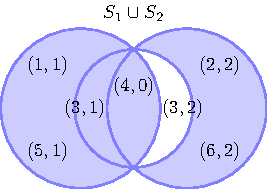
\includegraphics{fig_model_venn.pdf}
  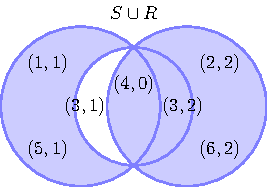
\includegraphics{fig_model_venn_reverse.pdf}
  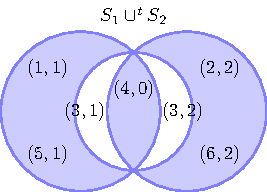
\includegraphics{fig_model_venn2.pdf}
  \caption{Venn diagrams for set and temporal set union operations of
    \acro{TSMS}}
  \label{fig:model:venn}
\end{figure}


\begin{example}\label{ex:model:s1s2}
  Let $R=\{(1,1), (3,1), (4,0), (5,1)\}$ and $S=\{(2,2), (3,2), (4,0),
  (6,2)\}$ be two time series. The union of $R$ and $S$ is $R\cup
  S=\{(1,1), (2,2), (3,1), (4,0), (5,1), (6,2)\}$. Because union is
  not symmetric, $S\cup R=\{(1,1), (2,2), \allowbreak(3,2), (4, 0), (5,1),
  (6,2)\}$. The temporal union results in $R\cupt S= S \cupt
  R=\{(1,1), (2,2), (4,0), (5,1), (6,2)\}$.  
  %
  Venn diagrams for all three cases are shown in
  Figure~\ref{fig:model:venn}, where the coloured area depicts the
  result time series. In every diagram, the central intersection area
  contains measures that share both time and value attributes, like
  instance $(4,0)$. The central left area contains the measures in $R$
  that only share the time attribute with a measure in $S$, like
  instance $(3,1)$. The central right area has a symmetrical
  meaning. The left and right outer areas are the remaining measures
  of $R$ and $S$ respectively.
\end{example}




Time series \emph{difference} can also be defined. Like union, the
difference requires both time series to have the same domain.
%
Let $R$ and $S$ be two time series and let $\dom R = \dom S$.
%
The \emph{difference} between $R$ and $S$, written $R-S$, is a time
series $R-S=\{m|m\in R\wedge m\notin S\}$.
%
The \emph{temporal difference} between $R$ and $S$, denoted $R-^t S$, 
is a time series $R-^t S=\{m|m\in R\wedge m \notinst S\}$.


Based on union and difference we can define \emph{intersection} as
$R\cap S = R - (R - S)$ and \emph{symmetric difference}
as $R \ominus S = (R - S) \cup (S - R)$. The
corresponding temporal operations can also be defined.


Relational \acro{DBMS} extend the set operators by some more such as
selection, rename or join. This kind of operators also make sense for
time series. To illustrate this possibility we define the join
operator.

Roughly speaking, the join of two time series is the combination of
measures sharing the same time attribute.  Let $R$ and $S$ be two time
series.  The \emph{join} of $R$ and $S$, denoted $R \join S$, is a
multivalued time series $R \join S = \{ (t,v_1,v_2) | (t,v_1) \in
R\wedge (t,v_2) \in S\}$. Note that $\dom(R\join
S)=\dom R\times\dom S$.
%
It must be noted that join requires both time series measures to share
exactly the same times. When time series diverge, the temporal
function operations explained later can be applied to adjust the time
instants to join requirements.


A \acro{DBMS} requires computational operators to provide opportunity
to calculate using the data contained. Relational \acro{DBMS} supply
operators like extend, aggregate or
summarise~\cite{date:introduction}. For time series, we define the more
general computational operators \emph{map} and \emph{fold}.

The map operator transforms a time series $S$ into a new time series
$R$ by applying a function to every measure.  Let $S$ and $R$ be two
time series, let $\cal{V}=\dom S$ and $\cal{V'}=\dom R$, and let
$f:\cal{T}\times\cal{V}\rightarrow\cal{T}\times\cal{V'}$ be a function
over a measure returning a measure. The \emph{map} of $f$ over $S$ is
a new time series defined as $\map(S,f)=\{f(m)|m\in S\}$. Note that
$\dom(\map(S,f))=\cal{V'}$.
%


The fold operator recursively combines every measure of a time
series. Assuming that $\mathcal{P}(C)$ is the powerset of $C$, we
define fold as follows.
%
Let $S=\{m_0,\dots, m_k\}$ and $R$ be two time series, let
$\mathcal{V}=\dom S$, let $\mathcal{V'}=\dom R$ and let 
%
$f:\mathcal{P}(\mathcal{T}\times\mathcal{V'}) \times (\mathcal{T}\times\mathcal{V}) \rightarrow \mathcal{P}(\mathcal{T}\times\mathcal{V'})$ 
%
be a function over a time series and a measure, which returns a time
series.
%
The \emph{fold} of $S$ by $f$ with initial value $R$ is a new time
series defined as $\fold(S,R,f) = f(\cdots(f(f(f(R,m_0),\allowbreak
m_1),\allowbreak m_2)\cdots),\allowbreak m_k)$.
%



The classical aggregation operator combines the data of a time series
into a single value.  It is worth to note that it is a special
case of fold.

Let $S=\{m_0,\dots,m_k\}$ be a time series, let $\mathcal{V}=\dom S$,
let $m$ be a measure with $\dom m=\mathcal{V}$, and let 
%
$f:(\mathcal{T}\times\mathcal{V})\times(\mathcal{T}\times\mathcal{V})\rightarrow \mathcal{T}\times\mathcal{V}$ 
%
be a function over two measures returning a measure. The
\emph{aggregate} of $S$ by $f$ with initial value $m$ is a new time
series defined as $\agg(S,m,f) = f(\cdots(f(f(f(m,m_0),\allowbreak
m_1),\allowbreak m_2)\cdots),\allowbreak m_k)$.  

% In the previous fold, the measures are computed in random order.
% However in some computational operations it is necessary to define the
% order, especially when $f$ is not commutative.  Then, it is possible
% to define a \emph{fold with order} as an extension of fold where
% measures are computed in a predetermined order.

% We define a
% \emph{fold with order}, $\orderfold$, as an extension of fold with a
% function $o$ that selects measures in order where $o: S_a \mapsto m_r$
% \[
%  \orderfold(S,S_i,f^f,o) =
%   \begin{cases}
%     S_i  \text{ if } |S|=0, \\
%     \orderfold(S_o,f^f(S_i,m_o),f^f,o)  \text{ else}
%   \end{cases}
% \]
% where $m_o = o(S)$ and $S_o = S - \{m_o\}$.



\begin{example}
\label{ex:computational-operators}
Let $S=\{(1,1),(2,3),(4,1)\}$ be a time series.  Map operator allows
computing a new time series whose values result from time multiplied
by value.  We define the map function $f(t,v)=(t,t\cdot v)$. Then
$\map(S,f)=\{(1,1),(2,6),(4,4)\}$.  
%


The aggregate operator allows, for instance, to compute the measure
that results from the sum of all the values.  To illustrate it, we
define the aggregate function $f(m,n)=(0,V(m)+V(n))$. Now,
$\agg(S,(0,0),f) = (0,5)$, where $5$ is the sum of all the values of
$S$. Note that time is meaningless in this computation.

The fold operator allows, for instance, to select the measures having
its value equal to one.  We define the fold function $f(R,m)=R\cup R'$
where $R'=\{m\}$ if $V(m)=1$ or $R'=\emptyset$ otherwise. Let $m$ be
any measure, note that $f(\emptyset,m)= R'$. Then
$\fold(S,\emptyset,f)=\{(1,1),(4,1)\}$.
\end{example}

%%%%%%% BINARY COMPUTATIONAL OPERATORS

Finally we describe how, using the operators defined before, we can
implement \emph{binary computational} operators between two time
series. This illustrates the power of the operators defined so far.
%

The strategy requires first to join the two time series and then
apply the computational operations. 
%
Let $S$ and $R$ be two time series and $\odot$ be a binary operator on
the value domain. The operator $\odot$ can be extended to the time
series as:
%
$S\odot R=\map(S\join R, f)$ being $f$ the function
$f(t,v,w)=(t,v\odot w)$.
%
This allows to extend real binary operations such as sum, $R+S$, or
division, $R/S$, to time series.


\subsubsection{Sequence operations}
\label{sec:sequence}

Sequence operations manipulate time series considering measures as
being totally ordered by time.  We define three basic operations:
\emph{slice}, \emph{successor} and \emph{concatenation}.


The classical interval concept can be applied to time domain. In this
context, given two time instants $s$ and $t$, we use the notation
$[s:t]$, $(s:t)$, $[s:t)$ and $(s:t]$ respectively for the closed
interval, open interval, open right and open left interval.
%
Following~\cite{last:hetland}, to slice a time series $S$ means to
extract a new time series $R\subseteq S$ constrained to a given time
interval. We denote this operation as the original time series followed
by the interval. Therefore, $S[s:t]=\{m|m\in S \wedge
T(m)\in[s:t]\}$. We can use other intervals to slice a time series in
a same fashion. For instance, $S(s:t]=\{m|m\in S \wedge
T(m)\in(s:t]\}$.

The ordinary time order allows to define the concepts of successor and
predecessor for the measures of a time series.
%
Let $S=\{m_0,\ldots,m_k\}$ be a time series and $m$ be an arbitrary
measure.
%
We say that $m_i=\nex_S(m)$ is the \emph{next} measure to $m$ in $S$ if and
only if $m_i=\inf(S(T(m):+\infty])$.  
%
We also say that $m_i=\prev_S(m)$ is the \emph{previous} measure to
$m$ in $S$ if and only if $m_i=\sup(S[-\infty:T(m)))$. 
%
Infinite measures are obtained when next and previous are applied to
supremum and infimum measures respectively: $\nex_S(\sup
S)=(+\infty,\infty)$ and $\prev_S(\inf S)=(-\infty,\infty)$.

To concatenate two time series means to compute a new time series with
the measures of the first time series followed in time order by the
measures of the second one. 
%
The concatenation requires both time series to share the same domain.
Let $R$ and $S$ be two time series and let $\dom R=\dom S$. The
\emph{concatenation} of $R$ and $S$, denoted as $R||S$, is a time
series that contains all the measures of $R$ together with those of
$S$ that do not intersect with the time interval of $R$. That is,
$R||S= R\cup (S - S[T(\inf R):T(\sup R)])$.



\subsubsection{Temporal function operations}
\label{sec:model:tfunc}

A time series can be thought as discrete representation of an
(original) temporal function. In this section we devise some
operations that manage the time series according to this temporal
function standpoint.  
%

The graph of a function allows to obtain and interpret the
continuous nature of a time series, when the domain of time and value
attributes can be plotted then the graph is equivalent to a graphical
representation.  
%
Let $S$ be a time series and $\cal{T}$ the time domain. The \emph{graph} of
the time series $S$ is a set of ordered pairs $\graph S
=\{(t,S(t))|t\in \cal{T}\}$ where $S(t)$ is a \emph{temporal representation
function} for the time series.
%


Given a time series $S$, the \emph{temporal representation function}
$S(t)$ is a function along the variable $t$ in the domain of
time and the target in the domain of values.
%
In some sense, $S(t)$ can be thought as the original temporal function
from which $S$ was obtained.
%

There is not an unique way to obtain $S(t)$ for a given time series
$S$. Because of this, in temporal representation functions we will
introduce a superscript, say $r$, that shows the name $r$ of the
representation method used. Then, $S(t)^r$ means the representation
function of $S$ using method $r$. Below, we exemplify the
representation functions using two different methods based on impulse
and constant piecewise functions.


\begin{definition}[Dirac representation] 
  Dirac delta (\dd) is a method of representation based on the Dirac
  delta function. Let $S$ be a time series. We define $S(t)^\dd$ as
  the following \dd{} representation function:
  \[
  S(t)^\dd
  =  \begin{cases}
          V(m) & \text{if } \exists m\in S:t=T(m) \\
          0    & \text{otherwise}
  \end{cases}
  \]
\end{definition}

\begin{definition}[Zohe representation]
  Zero-order hold everted (\zohe{}) is a method of representation
  based on the \emph{zero-order hold} signal reconstruction method. It
  is a piecewise constant function built from left-continuous step
  functions.  Let $S$ be a time series. We define $S(t)^\zohe$ as the
  following representation function:
  \[
  S(t)^\zohe 
  = \begin{cases}
    V(m) & \text{if } \exists m\in S: t\in \big(T(\prev_S(m)):T(m)\big]\\
    0    & \text{if } t > T(\max(S)) 
  \end{cases}
  \]
\end{definition}




The concept of representation is used for formalising some set and
sequence operators as temporal operators. 

% Consequently, the result of each one will depend on a representation
% method, which is indicated as a parameter.


We define a temporal interval operation to introduce this concept.
Let $S$ be a time series, let $[s:t]$ be an interval of two time
instants and let $r$ be a representation method. The \emph{temporal
  interval}, denoted as $S[s:t]^r$, returns a new time series with
measures in the interval temporal range. That is, $S[s:t]^r = S(u)^r$
for all $u \in [s:t]$. This is a general definition difficult to
implement, so for every representation a particular temporal interval
must be interpreted:

\begin{itemize}
\item Let $S(t)^\dd$ be the \dd{} representation for $S$. The
  \emph{\dd{} temporal interval} is $S[s:t]^\dd = S[s:t]
  \cup \{m\} \cup \{n\}$ where $m=(s,0)$ and $n=(t,0)$.

\item Let $S(t)^\zohe{}$ be the \zohe{} representation for $S$. The
  \emph{\zohe{} temporal interval} is $S[s:t]^\zohe{} = S(s:t]
  \cup \{m\}$ where $m=(t,v)$ and $v= V(\inf( S[t:+\infty] ))$.
\end{itemize}



From temporal interval other operators can be defined such as temporal
selection, temporal concatenation, or temporal join. As example the
definition of temporal interval operation is given.


The temporal selection over a time series allows to change the
resolution in the context of a representation function.  Let $S$ be a
time series, let $T=\{t_0,t_1,\dotsc,t_k\}$ be a set of time instants, and let 
$r$ be a representation method. The \emph{temporal selection}, denoted as
$S[T]^r$, is a time series with measures in $T$ times computed in
coherence with the representation method $r$. That is, $S[T]^r = S[t_0:t_0]^r
\cup S[t_1:t_1]^r \cup \dotsb \cup S[t_k:t_k]^r$. Let $t$ be a time
instant, note that temporal selection depends on the temporal interval
operation $S[t:t]^r$, which is equivalent to the notion of
temporal representation function over a single time instant. That is, $S[t:t]^r
= \{ (t, S(t)^r) \}$.




The temporal selection operation also allows to regularise a irregular
time series. Let $S$ be a time series, let $d,e\in\cal{T}$ be the
desired regularity parameters, and let $k\in\N$ be a limit for the
scope of the range.  A regularised $S$ can be obtained with $S[T]^r$
where $T = \{e+nd | n\in\N \wedge n\leq k \}$ is a set of time
instants equi-spaced.






\section{Multiresolution model}
\label{sec:MTSMS}

In this section we formalise a model for \acro{MTSMS}. Illustration
examples of the definitions given can be found at the end of the
section. Furthermore, in Section~\ref{sec:features} we have
intuitively introduced the concept of multiresolution through an
example.

A \acro{MTSMS} is a \acro{TSMS} that stores time series using a lossy
compression approach. 
%
The \acro{MTSMS} model is based on the concepts of \emph{measures} and
\emph{time series} as defined in Section~\ref{sec:model:TSMS}. We call
\emph{multiresolution time series} to each time series stored in a
\acro{MTSDB}.
%
A multiresolution time series is a collection of \emph{resolution
  subseries} that store a view of the original time series in a given
resolution.
%
The operator that adds data to a resolution subseries requires to
temporarily accumulate measures in a \emph{buffer}. This allow to
aggregate original data to obtain the expected resolution and finally
store them in a \emph{disc}.


\begin{figure}
  \centering
  %\begin{tikzpicture}
 \tikzset{
        myarrow/.style={->, >=latex',  thick},
      }
      

  \node[rectangle,draw,minimum height=6cm,minimum width=9cm] (m) {};
  \draw[shift=( m.south west)]   
  node[above right] {base de dades multiresolució};


  %discmig
  \node (m.center) (discr1) {...};

  %discr
  
  \node[ellipse,draw,minimum height=3.5cm,minimum width=2.5cm,alias=discr0] [left=of discr1] {};
  \node[above=0cm of discr0.north] {R0};
  \node[below=0cm of discr0] {disc resolució};

  \node[cylinder, draw, shape border rotate=90, aspect=0.25,alias=buffer0] [below=3mm of discr0.north] {buffer};
  \node[circle, draw,alias=disc0]  [above=3mm of discr0.south] {disc} ;
  \draw [->] (disc0.center)++(.4:.4cm) arc(0:180:.4cm);
  \draw[myarrow] (buffer0.bottom) -- (disc0.north);


  %discrd

  \node[ellipse,draw,minimum height=3.5cm,minimum width=2.5cm,alias=discrd] [right=of discr1] {};
  \node[above=0cm of discrd] {Rd};
  \node[below=0cm of discrd] {disc resolució};

  \node[cylinder, draw, shape border rotate=90, aspect=0.25,alias=bufferd] [below=3mm of discrd.north] {buffer};
  \node[circle, draw,alias=discd]  [above=3mm of discrd.south] {disc} ;
  \draw [->] (discd.center)++(.4:.4cm) arc(0:180:.4cm);
  \draw[myarrow] (bufferd.bottom) -- (discd.north);



  %mesura 
  \node[above=1cm of m.north] (m0) {};

  \draw[myarrow] (m0) -- (m.north) 
  node[right,midway] {mesura};

  \draw[myarrow] (m.north) -- (buffer0);
  \draw[myarrow] (m.north) -- (bufferd);
  \draw[myarrow] (m.north) -- (discr1);

\end{tikzpicture}
  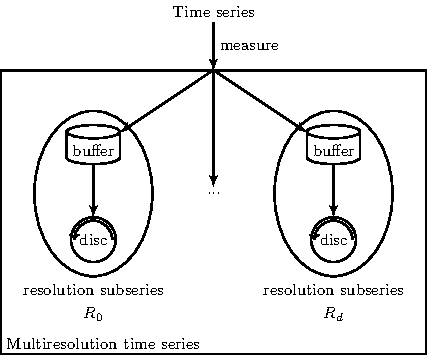
\includegraphics{fig_model_mtsdb.pdf}
  \caption{Architecture of \acro{MTSMS} model}
  \label{fig:model:mtsdb}
\end{figure}

Figure~\ref{fig:model:mtsdb} shows the architecture of a
\acro{MTSMS} for a single multiresolution time series.
%
In this way, the original time series gets stored in the resolution
subseries, each with a different time resolution and distinct
attribute aggregation policies. Discs are size bounded so they only
contain a fixed amount of measures. When a disc becomes full it
discards a measure. Thus, a multiresolution database is bounded in
size and the time series gets stored in a number of storage bounded
time subseries.

Regarding operations, the \acro{MTSMS} model requires two kind of
operators. Some operators should be devoted to set up the time
intervals between measures and to aggregate the attributes. Some other
operators should be dedicated to query the multiresolution schema and
to extract the time series data.

Following, we define the \acro{MTSMS} model structure and the
structural operators, the operations to query a multiresolution
schema, and the \emph{attribute aggregate functions}.  Although schema
manipulation operations could be defined, in this paper we exclusively
focus on structure and data query operators.


\subsection{Structure}

A \emph{buffer} is a container for a time series. The aim of the
buffer is to regularise the time series using a constant
\emph{resolution step} and an \emph{attribute aggregate function}.  We
name \emph{consolidation} to this action of regularisation.  Note that
the attribute aggregate functions are defined in
Section~\ref{sec:model:interpolador}.

\begin{definition}[Buffer]
  Let $S$ be a time series, let $\tau\in\cal{T}$ be the last
  consolidation time, let $\delta\in\cal{T}$ be the resolution step
  and let $f$ be an attribute aggregate function. We define a
  \emph{buffer} $B$ as the tuple $B=(S,\tau,\delta,f)$.
\end{definition}

An empty buffer is noted as $(\emptyset, t_0, \delta, f)$, that is an
empty time series, an initial consolidation time $t_0\in\cal{T}$, a
resolution step $\delta$ and a function $f$.  Given a buffer all the
consolidation time instants can be determined as $\tau_n=t_0+n\delta$
for all $n\in\N$.

Let $B=(S, \tau, \delta, f)$ be a buffer. The \emph{consolidation} of
$B$ is an operation that computes a new measure $m=f(S, \tau, \delta)$
summarising the data of $S$ comprised in the given interval.

A buffer has two main structural operations. The first one adds a
measure to the buffer and the second one consolidates the buffer.

Let $B=(S,\tau,\delta,f)$ be a buffer and let $m$ be a measure.  The
addition of $m$ to $B$, noted as $\addB(B,m)$, returns a new buffer
$\addB(B,m)=(S',\tau,\delta,f)$ where $S' = S \cup \{m\}$.

Let $B=(S,\tau,\delta,f)$ be a buffer. The consolidation of $B$, noted
as $\consB(B)$, returns a new buffer and a new measure $\consB(B)=(B',m')$
where $ B'= (S[\tau+\delta:+\infty], \tau+\delta,\delta,f)$ and $m' =
f(S,\tau,\delta)$. Note that after the consolidation, the
consolidated part of the time series can be removed from the buffer:
historic data is discarded.

The consolidation of a buffer is applied to the first non consolidated
time instant and the total consolidation is obtained by successive
application of the operator. 
%
This requires measures to be added by time order and to consolidate
the buffer when the time of some measure is bigger than the buffer's
next consolidation time.  
%
Let $B=(S,\tau,\delta,f)$ be a buffer and $m=\sup S$ the maximum
measure of $B$. We say that $B$ is consolidable if and only if $T(m)
\geq \tau+\delta$.

A \emph{disc} is a finite capacity container of measures. A time
series stored in a disc has its cardinal bounded. When the cardinal of
the time series is to overcome the limit, some measures need to be
discarded.

\begin{definition}[Disc]
  Let $k\in\N$ and $S$, $|S|\leq k$, be a time series. We define a
  \emph{disc} $D$ as the tuple $D=(S,k)$.
\end{definition}

An empty disc is noted as $(\emptyset,k)$. It is the tuple of an
empty time series and a bound $k$.

The main operation on a disc is to add a measure while keeping under
control the cardinal of the times series. Let $D=(S,k)$ be a disc and
let $m$ be a measure.  The addition of $m$ to $D$, written as
$\addD(D,m)$, is a new disc $\addD(D,m)=(S',k)$ where
%
\[
S' = \begin{cases}
  S\cup\{m\}                 & \text{if } |S|<k  \\
  (S-\{\min S\}) \cup \{m\} & \text{otherwise}
\end{cases}  
\]

A \emph{resolution subseries} is a structure that regularises and
aggregates a time series. It is composed of a buffer, which contains
the time series to be regularised, and a disc, which contains
the regularised time series.


\begin{definition}[Resolution subseries]
  Let $B$ be a buffer and let $D$ be a disc.  We define a
  \emph{resolution subseries} $R$ as the tuple $R=(B,D)$.  
\end{definition}
 
The operators of a resolution subseries extend the buffer and disc
ones. Let $R=(B,D)$ be a resolution subseries and let $m$ be new a
measure.  The addition of $m$ to $R$, noted as $\addR(R,m)$, is a new
resolution subseries $\addR(R,m)=(B',D)$ where $B'= \addB(B,m)$ is the
addition of the measure to the buffer.  The consolidation of $R$,
noted as $\consR(R)$, is a new resolution subseries
$\consR(R)=(B',D')$ where $(B',m') = \consB(B)$ is the consolidation
of the buffer and $D'= \addD(D,m')$ is the addition of the
consolidated measure to the disc. A resolution subseries is
consolidable only when its buffer is consolidable.

A \emph{multiresolution time series} is a set of resolution subseries
referred to the same time series. We store a time series regularised
with distinct resolutions across the resolution subseries, as
previously shown in Figure~\ref{fig:model:mtsdb}.

\begin{definition}[Multiresolution time series]
  Let $M=\{R_0, \dots, R_k\}$ be a finite set of resolution
  subseries. Then $M$ is a \emph{multiresolution time series}.
\end{definition}

Therefore, to define a multiresolution time series we must define the
number of resolution subseries and its corresponding parameters
$(\delta,\tau,f,k)$.  Usually there are no repeated pairs of
$(\delta,f)$ parameters among a multiresolution series, so they act as
key attributes.

The operators of a multiresolution time series apply to every
resolution subseries contained. Let $M=\{R_0,\allowbreak
\dots,\allowbreak R_k\}$ be a multiresolution time series and let $m$
be a measure.
%
The addition of a measure to every resolution subseries, noted as
$\addM(M,m)$, is a new multiresolution time series $\addM(M,m)=\{R'_0,
\dots,\allowbreak R'_k\}$ where $R'_i=\addR(R_i,m)$. The consolidation
of all resolution subseries, noted as $\consM(M)$ is a new
multiresolution time series $\consM(M)=\{R'_0,\allowbreak
\dots,\allowbreak R'_k\}$ where
\[R'_i=
\begin{cases}
\consR(R_i) & \text{if } R_i \text{ consolidable}\\
 R_i & \text{otherwise}
\end{cases}
\]

% The multiresolution consolidation operation should be applied
% regularly based on a consolidation clock. When the measure ordered
% addition approach is taken as explained in the buffer's consolidation,
% then there is no need for a clock in a \acro{MTSMS}. The consolidation
% clock is induced by the measure's addition and then it is only
% necessary to check the multiresolution consolidation operation on new
% additions. However, there could be other approaches where the
% consolidation clock was given by an external clock or external
% events. Then the consolidable definitions would depend on this
% external clock.





\subsection{Queries}

There are two basic time series queries for a \acro{MTSMS}: (i) to
extract a time subseries from a resolution subseries or (ii) to query
for a total time series from all consolidated data.

% Aquesta sembla una consulta una mica circumstancial i menor ...
Let $M$ be a multiresolution time series and let $(\delta,f)$ be a
pair of key attributes.  The first query, denoted as
$\seriedisc(M,\delta,f)$, is a time series such that $\exists (B,D)
\in M: B=(S,\tau,\delta,f) \wedge D=(\seriedisc(M,\delta,f), k) $
where $S,\tau,k$ are bound variables.  Note that we
assume there are no repeated $(\delta,f)$ pairs in $M$.

Let $M=\{R_0,\dots,R_k\}$ be a multiresolution time series and let
$S_0,\dots,S_k$ the time series corresponding to the resolution
subseries $R_0,\dots,R_k$. Assume that the attribute aggregation
functions of all $R_i$ are the same and the resolution steps of all
$R_i$ are distinct.
%
We note as $\totalseries(M)$, the time ordered concatenation of all
time subseries. Recall that $R||S$ is the concatenation for two time
series $R$ and $S$, which has been defined in
Section~\ref{sec:sequence}. Assume that $i_0,\dots,i_k$ is a
permutation of $[0,k]$ such that $\delta_{i_0} < \delta_{i_1} < \cdots
< \delta_{i_k}$ being $\delta_i$ the resolution step of the resolution
subseries $R_i$. Then, $\totalseries(M) = S_{i_0} || S_{i_1} || \cdots
|| S_{i_k}$.
%
TotalSeries obtains the better possible resolution.

From these aforementioned basic time series queries, more elaborated
queries can be applied to \acro{MTSMS} by using \acro{TSMS}
operations. For example, let $L$ and $M$ be two multiresolution time
series, we can compute the sum of both as $\totalseries(L) +
\totalseries(M)$. Recall that $R+S$ is the sum of the values of two
time series $R$ and $S$, which has been defined in
Section~\ref{sec:set} as a binary computational operator.


\subsection{Attribute aggregate function}
\label{sec:model:interpolador}

Attribute aggregate functions are a specific case of \acro{TSMS}
aggregate operations used to summarise time series data while
consolidating a buffer.
%
% Let $S$ be a time series and let $[x,v]$ be a
% time interval. An attribute aggregate function $f$ calculates a new
% measure $m=f(S,[x,v])$. Then, this resulting measure $m$ is interpreted to
% summarise the measures of $S$ for the consolidation interval $[x,v]$.

Let $S$ be a time series, let $\delta$ be a resolution step and let
$\tau$ be a consolidation time.  An \emph{attribute aggregate function} $f$
calculates a new measure $m=f(S,\tau,\delta)$. From $\tau$ and
$\delta$, we obtain the time interval $[\tau:\tau+\delta]$.  Then, the
resulting measure $m$ is interpreted to summarise the measures of $S$
for the time interval $[\tau:\tau+\delta]$.



% \[
% f : S=\{m_0,\ldots,m_k\} \times I=[t_i,t_j] \mapsto m'
% \]
% \[
% f: \cal{P}(\cal{T}\times\cal{V}) \times (\cal{T}\times\cal{T}) \rightarrow \cal{T}\times\cal{V}
% \]

An attribute aggregation function follows this general schema. First,
it obtains a time subseries $S'$ according to the consolidating
interval using a slice operator. For example, $S' =
S[\tau:\tau+\delta]$. Second, it applies a \acro{TSMS} aggregation
function on this time subseries to obtain $m$. For instance, $m =
\agg(S',n, f)$, being $f$ an aggregation function and $n$ an initial
measure, as defined in Section~\ref{sec:set}.

Many different attribute aggregate functions can be used in order to
summarise a time series, for example it is possible to calculate an
statistic indicator of the time series such as the average or a more
complex digital signal processing operation as proposed
by~\cite{zhang11}. Furthermore, the representation of a time series
and some of its pathologies can be considered during the aggregation
process.

Given the diversity of attribute aggregate functions, no global
assumptions can be made about them. Each user should decide which
combination of aggregation and representation fits better to the
measured phenomena.  Therefore, the \acro{MTSMS} model must have a
generic design that allows the users to define their own aggregate
functions.

In what follows we will give some examples of usual attribute
aggregation functions. These functions compute a new measure given a
set of known measures. Then, an attribute aggregation function should
compute a new \emph{time} and a new \emph{value} from the set known measures.
%
% For the rest of this Section we will write $m=f(S,[x,v])$ be the
% resulting measure of an attribute aggregation function $f$ applied to
% a time series $S$ for a time interval $[x,v]$.

% Sobre el calcul del nou temps

The attribute aggregation functions generally return measures that
match the buffer consolidating times. Assume, for instance, that $f$
is an attribute aggregation function and let $m=f(S,\tau,\delta)$.
Then, the time of $m$ is usually computed as $T(m)=\tau+\delta$.
%
However, in some cases it is preferred that $T(m)$ do not match the
buffer consolidating times.
%
For instance, the resulting measure can be aggregated from a time
subseries $S'$ using an open interval $S'=S(\tau:\tau+\delta)$, a
closed interval $S'=S[\tau:\tau+\delta]$, or other combinations like
$S'=S(\tau-d:\tau+\delta-d]$, where $d$ is a time duration that delays the
consolidation to $T(m)=\tau+\delta-d$.
%
This time offset can also be variable. For example, an aggregate
function that returns the first measure of the interval
$m=\min(S[\tau:\tau+\delta))$, then the resulting time fulfils that
$\tau\leq T(m) < \tau+\delta$.

% Sobre el calcul del nou valor
Assume that $f$ is an attribute aggregation function and let
$m=f(S,\tau,\delta)$.  An attribute aggregation function $f$ should
compute the value of $m$.
%
Next there are some examples that illustrate how to compute $V(m)$
based on the temporal function time series operators. 
That is, the time series aggregated is interpreted by the temporal
representation function $S(t)^r$ as has been described in
Section~\ref{sec:model:tfunc}. 
%
In these example functions we leave the time series representation $r$
uninstantiated.

\begin{itemize}
\item The \emph{maximum} computes $V(m)$ as $V(m) =
  \max\limits_{\forall t \in [\tau:\tau+\delta]} S(t)^r$. It
  summarises $S$ with the maximum of the measure values in the
  interval $[\tau:\tau+\delta]$.
\item The \emph{last} computes $V(m)$ as $V(m) = S(\tau+\delta)^r$. It
  summarises $S$ with the value at $\tau+\delta$ time instant.
\item The \emph{mean} computes $V(m)$ as $V(m) = \frac{1}{\delta}
  \int\limits_{\tau}^{\tau+\delta} S(t)^r dt$. It summarises $S$ with
  the mean of the function in the interval $[\tau:\tau+\delta]$.
\end{itemize}

The time series representation in previous examples can be
instantiated in several ways. In what follows we exemplify this
instantiating $r$ as \dd{} and \zohe{}.

Dirac delta attribute aggregation functions interpret the resulting
time as centered on the interval $T(m)=\frac{2\tau+\delta}{2}$. The
resulting value $V(m)$ depends on the attribute, let
$S'=S[\tau:\tau+\delta]^\dd$ be the selection of measures by Dirac
delta temporal interval. Then,
\begin{itemize}
\item The $maximum^\dd$ is such that $V(m) =
  \max\big(0,\max\limits_{\forall n \in S'} V(n)\big)$.
\item The $last^\dd$ is such that $V(m) = V(\max S')$.
\item The $mean^\dd$ is such that $V(m) = \frac{1}{\delta}
  \sum\limits_{\forall n \in S'} V(n)$. Note that for the Dirac
  delta function $\int\dd(t)dt=1$.
\end{itemize}

Note that $\sum\limits_{\forall n \in S'} V(n)$ is a sum of values
that could be implemented as $\agg(S',(0,0),f)$ where
$f(m,n)=(0,V(m)+V(n))$, as shown in
Example~\ref{ex:computational-operators}.

\zohe{} attribute aggregation functions interpret the resulting time
as the right limit of the interval $T(m)=\tau+\delta$. The resulting
value $V(m)$ depends on the attribute, let
$S'=S[\tau:\tau+\delta]^\zohe{}$ be the selection of measures by
\zohe{} temporal interval. Then,

\begin{itemize}
\item The $\maxz$ is such that $V(m) = \max\limits_{\forall n \in S'}
  V(n)$.
\item The $last^\zohe{}$ is such that $V(m) = V(\max S')$.
\item The $\meanz$ is such that $V(m) = \frac{1}{\delta}
  \big[(T(o)-\tau)V(o) + \sum\limits_{\forall n\in R}( T(n)-
  T(\prev_S n) )V(n)\big]$ where $o=\min S'$ and $R= S' - \{o\}$.
\end{itemize}

Note that  $\meanz$ is a sum of values
that could be implemented as $\meanz = \frac{1}{\delta}\agg(S',(0,0),f)$ where $f(m,n)=(0,V(m)+v)$ and 
\[
 v= 
 \begin{cases}
   (T(n)-\tau)V(n) & \text{if } n=\min S'\\
   (T(n)-T(\prev_{S'} n))V(n) & \text{else }
 \end{cases}
\]

\emph{RRDtool}, \cite{rrdtool}, uses an aggregation function similar
to $\meanz$ to summarise velocity counter data by keeping the area
below the original signal.

It is interesting to note that some attribute aggregation patterns are
very similar. For instance, the maximum and last attribute aggregation
schemes differ basically on the interval selection operation. However,
other patterns have a more elaborated interpretation depending on the
actual representation used. This is the case of $\meanz$ and $mean^\dd$.


\begin{example}\label{ex:model:smultiresolution} 
  We define a multiresolution schema for a time series, we consolidate
  the database and we query its data.  Let $S = \{
  (1,6),(5,2),\allowbreak (8,5),\allowbreak (10,0),\allowbreak
  (14,1),\allowbreak (19,6),\allowbreak (22,11),\allowbreak
  (26,6),(29,0) \}$ be a time series and let $M=\{R_0,R_1\}$ be a
  multiresolution time series where each resolution parameters are
  $\tau_0=0$ , $\delta_0=5$, $f_0 =\meanz$, $k_0=4$ and $\tau_1=0$,
  $\delta_1=10$, $f_1 =\maxz$, $k_1=2$. Therefore $R_0$ will be
  consolidated at time instants 5, 10, 15, 20, 25, 30\dots and $R_1$
  at 10, 20, 30\dots

  All measures of $S$ are added to $M$
  and then it is consolidated until it is no more consolidable. As
  $T(\max S)=29$, the last consolidation times are $\tau_0=25$ and
  $\tau_1=20$, so we call $M_{29}$ to the multiresolution time series
  at this state.

  Then, the two time subseries consolidated are obtained by querying
  $\seriedisc(M_{29},5,\allowbreak \meanz)=\{\allowbreak
  (10,3),\allowbreak (15,\allowbreak 2),\allowbreak (20,7),\allowbreak
  (25,8)\}$ and $\seriedisc(M_{29},\allowbreak 10,\allowbreak \maxz)
  =\allowbreak \{ \allowbreak (10,6),\allowbreak (20,11)\}$. Regarding
  buffers, let $S_0$ and $S_1$ be the $M_{29}$ buffer's time series,
  note that $S_0= \{\allowbreak (26,6),\allowbreak (29,0)\allowbreak
  \}$ and $S_1=\{\allowbreak (22,11),\allowbreak (26,6),(29,0)\}$.

  In this particular example,
  $ \totalseries(M_{29}) = \seriedisc(M_{29},\allowbreak 5,\meanz)$ as $R_0$ has
  twice the resolution than $R_1$ and $k_0$ is bigger than $k_1$. 
\end{example}



%%% Local Variables:
%%% TeX-master: "main"
%%% ispell-local-dictionary: "british"
%%% End:

% LocalWords:  genericity multiresolution subseries consolidable

% LocalWords:  pathologies MTSMS TSMS cardinality multivalued infimum
% LocalWords:  multivalues supremum tuple affinely projectively MTSDB
%  LocalWords:  semitemporal piecewise TotalSeries RRDtool



\chapter{Model SGST}
\label{cap:model:sgst}


En aquest capítol es defineix un model per als sistemes de gestió de
bases de dades per a sèries temporals (SGST). Aquest model
s'estructura en base a dos objectes principals, mesures i sèries temporals.
Ambdós tenen un atribut de temps, el qual requereix un tractament
adequat. El model de SGST es dissenya en tres parts.

\begin{itemize}

\item Primer, es defineix el model d'estructura de les dades, és a
  dir, la forma com es descriuen les mesures i les sèries temporals.  

\item Segon, es defineix el model d'operacions sobre les dades, és a
  dir, els operadors bàsics que permeten modelar el comportament i la
  manipulació de les sèries temporals.

\item Tercer, es descriuen propietats de les sèries
  temporals. Les sèries temporals adquireixen propietats
  variades depenent del context on s'apliquin.

\end{itemize}





\section{Model estructural de dades}

Una sèrie temporal és una relació de temps i valors. A cada parella
temps-valor l'anomenem mesura. Així doncs, una sèrie temporal és un
conjunt de mesures. 


En el nostre cas concret, una mesura es correspon amb un valor mesurat
en un instant de temps i una sèrie temporal esdevé una co\l.lecció de
mesures.





\subsection{Temps}
\label{sec:sgst:temps}

El temps és la variable que ens permet ordenar les mesures.  A tal
efecte, si denominem $T$ el domini del temps, els seus membres
presenten una relació d'ordre total. $T$ pot ser tant un conjunt finit
com infinit i normalment serà un conjunt tancat %(compactificat?)
per a poder incloure les mesures indefinides (v.\
\autoref{def:model:mesura_indefinida}) com a límits.

Per tal de facilitar la comprensió, en el document utilitzarem el
conjunt de reals com a conjunt pels temps. Representarem el conjunt
$T$ amb el conjunt estès de nombres reals $\bar{\R{}} \in
\R{} \cup
\{+\infty,-\infty\}$, \parencite{wiki:extendedreal,cantrell:extendedreal},
també anomenat recta real acabada, el qual és un conjunt tancat.

El conjunt estès de nombres reals té dos punts límits corresponents al
valor impropi infinit, aleshores en notació d'interval el conjunt $T$
es pot escriure com $\bar{\R{}} \in [-\infty,+\infty]$. En referència
amb el conjunt dels nombres reals $\R{}$, les relacions d'ordre i
algunes operacions aritmètiques s'estenen al conjunt $\bar{\R{}}$,
\cite{cantrell:extendedreal}.  Algunes expressions esdevenen
indefinides (p.ex.\ $0/0$) i altres depenen del context, com és el cas
de l'expressió indeterminada $0 \times \infty$ que per exemple en la
teoria de la mesura habitualment es defineix com $0 \times \infty =
0$, \cite{wiki:extendedreal}.


El conjunt dels reals és un espai mètric ja que té definida una funció
distància (o mètrica), com per exemple la distància euclidiana. Com a
conseqüència, ens permet distingir entre instants de temps (els
elements del conjunt) i durades (la mètrica). Observant els instants
de temps com a punts en la recta real, les durades com a segments de
la recta real i especificant un instant de temps com a marc de
referència, es pot definir el temps com a sistema de
coordenades \parencite{iep:time-supplement,wiki:coordinate,kopetz11:realtime}. A
continuació definim el temps de manera que puguem ordenar
esdeveniments, mesurar durades d'esdeveniments i establir quan
esdevenen; és una aproximació ingènua sense abastar detalls complicats
del concepte temps \parencite{iep:time}.

\todo{s'hauria de dir que kopetz també en fa una definició similar}



\begin{definition}[Temps]
  \label{def:model:temps}
  Siguin $t^i_i$ i $t^i_j$ dos instants de temps amb el mateix $t^R$
  com a marc de referència, definim la quantitat de temps o la durada
  $t^d$ com un valor $t^d \in\bar{\R{}}$ que mesura la distància en
  unitats de temps entre dos instants de temps $t^d = d(t^i_i,t^i_j)$
  a on $d$ és la mètrica del conjunt $T$. En el cas que els instants
  de temps es defineixin com a reals, $t^i_i , t^i_j \in \bar{\R{}}$,
  aleshores $t^d = t^i_i - t^i_j$.

  Sigui $T$ el domini del temps, definim un instant de temps $I$ com
  un element del conjunt $I \in T$. Així, un instant de temps és
  l'etiqueta d'un punt en la línia temporal. Seguint la definició de
  sistema de coordenades i prenent els nombres reals com a domini del
  temps, sigui $t^{R}$ un instant de temps marc de referència,
  aleshores els instants de temps es defineixen com un valor $t^i
  \in\bar{\R{}}$ que indica la distància de temps amb signe respecte a
  l'instant de temps de referència $t^i= d(t^{R},I)$ a on $d$ és la
  mètrica del conjunt $T$.
\end{definition}

En resum, els instants de temps es poden veure com una seqüència de
valors reals que indiquen esdeveniments amb ordre clarament definit i
entre dos instants de temps sempre hi ha una durada. Expressarem tant
els instants de temps com les durades amb un real que té unitats de
temps. Aquestes unitats són 'segons' en sistema internacional.

% El marc de referència és un instant de temps que permet definir
% unívocament la posició de qualsevol altre instant de temps en un
% sistema de coordenades.



\subsubsection{Estàndards de temps}

Els estàndards de temps especifiquen com s'ha de mesurar el pas del
temps i com s'han d'assenyalar els instants de temps.
\textcite{allen:timescales} recull diferents estàndards de temps
que existeixen, dels quals a continuació comentem els més habituals.

Actualment l'estàndard de temps habitual per mesurar el pas del temps
és el Temps Atòmic Internacional (TAI), del qual se'n deriva un altre
estàndard més conegut que és el Temps Universal Coordinat (UTC).
Ambdós estàndards assenyalen el instants de temps segons el calendari
Gregorià i el calendari julià. Actualment, de forma genèrica s'utilitza
UTC per a sincronitzar rellotges tot i que en el futur es podria
canviar per un nou estàndard, el Temps Internacional (TI), el qual
també es base en el TAI.

El calendari julià utilitza un estàndard de comptar el temps com a
nombre de dies que han passat des d'una data concreta, la qual
s'anomena època. L'època es correspon amb el concepte d'instant de
temps marc de referència de la \autoref{def:model:temps}. Per defecte
l'època se situa a l'inici del Període Julià tot i que també se solen
utilitzar altres dates assenyalades.

Un altre estàndard semblant al julià és l'Hora POSIX o Hora Unix, el
qual compta el nombre de segons des de l'1 de gener de 1970 basant-se
en el les mesures d'UTC. L'Hora Unix és l'estàndard de temps habitual
en els sistemes operatius de la família Unix. No obstant, aquest
estàndard presenta un problema d'ambigüitat a causa que no té no té en
compte els segons addicionals d'UTC.





\subsubsection{Calendari}

Un cas particular del temps és el calendari. Els calendaris són
definicions pel domini temps que consisteixen en noms per als punts de
la línia de temps i regles per establir la durada entre ells per tal
de que el temps tingui certa relació amb la rotació de la Terra. A
l'apartat anterior hem definit el domini temps de manera general
amb el conjunt de reals, els quals exemplifiquen més clarament el
concepte de sistema de coordenades de temps absolut.

\textcite{dreyer94} situen els calendaris i les seves operacions com a
essencials en els SGST. Tanmateix, pot no ser necessari modelar les
dates i regles de calendari en el model de temps. Els calendaris es
poden observar com a noms que fan referència a instants de temps
quantificables, com els de la \autoref{def:model:temps}. Aleshores,
només cal una eina que sigui capaç de convertir els noms de calendari
a instants de temps.

El fet de que un calendari sigui més o menys complicat no afecta al
model de SGST, sols té incidència en les funcions de conversió
d'instant de temps a calendari i viceversa. Tampoc afecta que els
calendaris siguin ambigus (p.ex.\ dos noms per al mateix instant o
instants sense nom) o que continguin propietats impredictibles (p.ex.\
cas dels segons addicionals en UTC) ja que aquests casos es
corresponen amb la bona definició dels sistemes de calendari.

Així doncs, els calendaris en el model de SGST es poden implementar
com una extensió del model de temps. El tipus de dades ordinal de
calendari Gregorià implementat per
\textcite[cap.~16]{date02:_tempor_data_relat_model} pot servir com a
guia per a la implementació dels calendaris en els SGST.




\subsection{Valor}
\label{sec:sgst:valor}

\todo{T: refer tota la secció}

El \gls{terme:SGBDR:valor} és qualsevol element que és d'un
\gls{terme:SGBDR:tipus}; és a dir, un objecte que
pertany a un determinat conjunt de valors i que té associat les
operacions que s'hi poden aplicar. Exemples de tipus de dades són els
enters, els reals, les cadenes de text i les estructures de dades com
vectors, llistes o \glspl{terme:SGBDR:relacio}.  

\todo{Exemplificar més amb tipus que tenen valors i operacions que se'ls poden aplicar}

%\todo{potser citar que el valor es tracta de manera semblant a l'extensió del model objecte-relacional?}

El model de dades dels valors ha d'incloure una dada que defineixi el
valor indefinit. Més endavant a la
definició~\ref{def:model:mesura_valor_indefinit} es detallen les
propietats de les mesures amb valor indefinit. Seguint l'exemple amb
els reals, el valor indefinit es defineix amb el valor impropi infinit
del conjunt dels reals estès
projectivament, \parencite{cantrell:projectivelyextendedreal},
$\R{}^*\in\R{} \cup \{\infty\}$.


En aquest exemple amb reals, el valor és un escalar però fàcilment es
pot estendre el concepte a valors multivaluats ${\R{}^*}^n$ que
representin una co\l.lecció de valors mesurats en el mateix instant de
temps, tal i com fa per exemple \textcite{assfalg08:thesis}.







\subsection{Mesura}\label{sec:model:mesura} 

Una mesura està formada per la parella de temps i valor.

\begin{definition}[Mesura]
  \label{def:model:mesura}
  Definim \emph{mesura} com el tuple $(t,v)$, en el que $v$ és el
  valor de la mesura i $t$ és l'instant de temps en que s'ha pres
  aquesta mesura.
\end{definition}


Donada una mesura $m=(t,v)$ escriurem $V(m)$ per referir-nos a $v$ i
$T(m)$ per referir-nos a $t$.

L'instant de temps de les mesures indueix una relació d'ordre entre
les mesures.
\begin{definition}[Relació d'ordre]\todo{dir-li temporal, perquè sinó després $m\in S$ queda com $m\in^tS$. Arreglar-ho a les definicions de pertinença }
  \label{def:model:mesura-relacio-ordre}
  Sigui $m=(t_m,v_m)$ i $n=(t_n,v_n)$, direm que l'ordre de la mesura
  $m$ és major o igual que $n$, $m\geq n$, si i solament si $t_m\geq
  t_n$.
\end{definition}\todo{també hem de definir l'ordre parcial $m<n$ per la definició de pertinença no temporal?}


En les definicions de temps i valor s'han estès els conjunts amb
valors impropis, concretament s'ha exemplificat amb el conjunt estès
de nombres reals afí $\bar{\R{}} \in \R{} \cup
\{+\infty,-\infty\}$ i amb el projectiu $\R{}^*\in\R{}
\cup\{\infty\}$,
\parencite{cantrell:extendedreal,cantrell:projectivelyextendedreal}. Aquesta
extensió amb l'element impropi infinit ($\infty$) dóna com a resultat
unes mesures impròpies que anomenarem mesura de valor indefinit i
mesura indefinida.\todo{potser s'hauria de dir de no confondre el valor indefinit amb l'absència de valor; és a dir que en una sèrie temporal les mesures que no hi són, són absents (no s'han pres) i les mesures de valor indefinit s'han pres però tenien un valor erroni o desconegut (més a la secció de patologies).} 

\begin{definition}[Mesura de valor indefinit]
  \label{def:model:mesura_valor_indefinit}
  Definim \emph{mesura de valor indefinit} com el tuple $(t,v)$, en el
  que el valor és $v=\infty$ i l'instant de temps és
  $t\in\bar{\R{}}$.
\end{definition}

\begin{definition}[Mesura indefinida]
  \label{def:model:mesura_indefinida}
  Definim \emph{mesura indefinida} com el tuple $(t,v)$, en el que el
  valor és $v\in\R{}^*$ i l'instant de temps és
  $t\in\{+\infty,-\infty\}$.
\end{definition}

Així doncs, donada una mesura $m$, s'anota la mesura de valor
indefinit com $m=(t,\infty)$ i les mesures indefinides com
$m=(+\infty,v)$ per la positiva i $m=(-\infty,v)$ per la negativa, les
quals normalment s'anotaran també amb valor indefinit:
$m=(+\infty,\infty)$ i $m=(-\infty,\infty)$ respectivament.


Les mesures de valor indefinit es podran utilitzar en aquells casos en
els que el valor de la mesura és desconegut. Els valors desconeguts
són aquells valors que no existeixen (es desconeixen, \emph{missing
  data} ) o que s'ignoren (es descarten, \emph{censoring} o
\emph{truncation}). Els valors que no existeixen prenen el valor
desconegut en el moment de la mesura, en canvi els valors descartats
són marcats com a desconeguts després d'un processament de les dades.

Nota: en alguns sistemes es distingeix entre valors infinits
($\infty$) i valors indefinits (NaN, \emph{not a number}),
\cite{wiki:ieee754}. Aquest no és el cas de les definicions de mesures
indefinides presents.







\subsection{Sèrie temporal}
\label{sec:model:serietemporal}

Les sèries temporals són seqüències de mesures ordenades en el temps.
Tradicionalment s'anomenen sèries temporals tot i que alguns autors les anomenen
seqüències temporals, per exemple a \cite{last:hetland}.  Les sèries
temporals són mesures del mateix fenomen i com a conseqüència el tipus
dels valors de les sèries temporals és homogeni.


\begin{definition}[Sèrie temporal]
  \label{def:serie_temporal}
  Una sèrie temporal $S$ és un conjunt de mesures
  $S=\{m_0,\ldots,m_k\}$ sense temps repetits en la qual
  $\forall i,j: i\leq k, j\leq k, i\neq j : T(m_i)\neq T(m_j)$.
\end{definition}

Per ser un conjunt, les sèries temporals tenen mesura de cardinalitat.
\begin{definition}[Cardinal]
  Sigui $S=\{m_0,\ldots,m_k\}$ una sèrie temporal, definim el nombre
  de mesures que conté la sèrie temporal com el cardinal del conjunt
  $|S|=k+1$. Una sèrie temporal sense mesures és la sèrie temporal
  buida $S_\emptyset= \emptyset = \{\}$, és a dir que no té cap element
  $|S_\emptyset|=0$.
\end{definition}



 
\subsubsection{Formes d'una sèrie temporal}

Una sèrie temporal pot tenir formes diferents segons com s'expressi.
A continuació diferenciem entre tres formes possibles d'una sèrie
temporal: canònica, multivaluada i doble.


La forma bàsica d'una sèrie temporal és la de parelles de temps i
valor a la qual anomenem forma canònica.
\begin{definition}[Forma canònica]
  Sigui $S = \{ m_0, m_1 , \dotsc, m_k \}$ una sèrie temporal,
  s'escriu com $S =  \{
  (t_0,v_0), (t_1,v_1), \dotsc, (t_k,v_k)\}$; és
  a dir com a parelles de temps i valor. A aquesta
  forma l'anomenem canònica.
\end{definition}


Les sèries temporals poden mesurar alhora més d'un fenomen quan
aquests comparteixen els instants de temps de mesura. Aquestes sèries
temporals tenen forma de sèrie temporal multivaluada.

\begin{definition}[Sèrie temporal multivaluada]
  Anomenem sèrie temporal multivaluada a una sèrie temporal que té més
  d'un atribut de valors.  Sigui $S = \{ m_0, m_1 , \dotsc, m_k \}$
  una sèrie temporal és multivaluada si cada mesura $m_i$ és un tuple
  $m_i=(t,v_1,v_2,\dotsc,v_n)$ a on $t$ és un instant de temps i
  $v_1$, $v_2$, \dots, $v_n$ són valors. 

  Una sèrie temporal multivaluada es pot escriure en forma canònica de
  parelles $(t,v)$. És a dir, la sèrie temporal multivaluada en
  forma canònica té mesures $m_i$ com a tuples
  $m_i=(t,(v_1,v_2,\dotsc,v_n))$
\end{definition}

La forma canònica s'utilitza per a generalitzar les sèries temporals
multivaluades en les operacions on el valor multivaluat no és
rellevant. En altres operacions, per exemple la selecció o la junció,
el multivalor és rellevant per treballar-hi o perquè el resultat és
una sèrie temporals multivaluada. 



Hi ha una forma no habitual de les sèries temporals que es dóna quan
tenen dos atributs de temps i a la qual anomenem forma doble.

\begin{definition}[Sèrie temporal doble]
  \label{def:sgst:st-doble}
  Anomenem sèrie temporal doble a una sèrie temporal que té dos
  atributs de temps i dos atributs de valors. Sigui $S =\{m_0, \dotsc,
  m_k\}$ una sèrie temporal és doble si cada mesura $m_i$ és un tuple
  $m_i=(t_1,v_1,t_2,v_2)$ a on $t_1$ i $t_2$ són instants de temps i
  $v_1$ i $v_2$ són valors. De la mateixa manera, a aquesta mesura
  $m_i$ l'anomenem mesura doble.  Una sèrie temporal doble no té dues
  parelles de temps repetides $|\{(t_1,t_2) | t_1,t_2\in S\}| = |S|$.
\end{definition}

La sèrie temporal doble prové d'un producte de dues sèries
temporals. Està pensada com a càlcul intermedi d'altres operacions com
per exemple la junció o el mapatge. 
% La seva forma canònica es
% correspondria de manera semblant a l'exemple de la
% \autoref{fig:model:serietemporal:serietemporal}.









\subsubsection{Relació sèrie temporal}

Una sèrie temporal s'expressa com un conjunt i com a tal és
susceptible d'aplicar-hi els conceptes del model relacional dels
SGBD. A continuació, el que s'ha descrit a l'apartat anterior es torna
a expressar seguint el concepte de relació.


Per ser un conjunt de mesures, s'observa una sèrie temporal com una
relació de grau dos a on la capçalera conté els atributs temps i
valor. Ambdós atributs tenen els dominis de temps i valor descrits a
les seccions \ref{def:model:temps} i \ref{sec:sgst:valor}, com per
exemple el tipus de dades 'reals estesos'. Les relacions de sèries
temporals inclou algunes restriccions més que les relacions:

\begin{itemize}
\item Els temps no poden estar repetits: (\emph{key restriction \{t\}})
\item L'atribut de valor ha de contenir el mateix tipus d'objecte i ha
  d'estar associat al mateix fenomen o fenòmens.
\end{itemize}

Els temps no repetits indueixen un ordre temporal a les sèries
temporals. Tot i així, les relacions, per ser conjunts, conserven la
no definció d'un ordre dels elements. En el model relacional no hi ha
ordre ni en les tuples ni en els atributs a diferència de les
relacions matemàtiques que tenen un ordre d'esquerra a
dreta \parencite[sec.\ 5.3]{date:introduction}.


%\subsubsection{Possibles representacions}

A l'apartat anterior s'han descrit diverses formes d'una sèrie
temporal.  A continuació atenem a les possibles representacions com a
relació d'una sèrie temporal segons les formes que tinguin.

% Com a relació seguint el concepte de possibles
% representacions proposat per \textcite[cap.~5]{date:introduction} ?
% i les formes normals de les relacions [Date]?



\begin{definition}[Representació canònica]
  Sigui $S = \{ m_0, m_1 , \dotsc, m_k \}$ una sèrie temporal amb
  domini $\bar{\R{}}$ pels temps i els valors de les mesures,
  representada com a relació s'escriu com $S = ( \{t: \bar{\R{}}, v:
  \bar{\R{}}\}, \{ \{t:t_0,v:v_0\}, \{t:t_1,v:v_1\}, \dotsc,
  \{t:t_k,v:v_k\} \} )$; és a dir com a parella capçalera i conjunt de
  valors certs. A aquesta representació l'anomenem forma canònica.

  Així doncs, sigui $S_{\emptyset} = \{ \}$ una sèrie temporal buida,
  modelada com a relació s'escriu com $S_{\emptyset} = ( \{t:
  \bar{\R{}}, v: \bar{\R{}}\}, \{ \} )$.
\end{definition}


Degut al format esquemàtic de les sèries temporals, en simplifiquem
l'escriptura de la forma canònica com a conjunt de tuples $(t,v)$ a on
$t$ és el temps i $v$ és el valor. Així doncs quan no hi ha dubte
sobre els dominis ni els noms d'atributs, una sèrie temporal es pot
escriure de manera simplificada com a $S = \{ (t_0,v_0), (t_1,v_1),
\dotsc, (t_k,v_k) \}$, la qual es correspon amb la forma canònica de
la sèrie temporal representada com a conjunt.

Tal com s'utilitza en les relacions, les sèries temporals es poden
visualitzar com a taules. La sèrie temporal $S$ i la $S_{\emptyset}$
es visualitzen com a taula a la
\autoref{fig:model:serietemporal:taula}.

\begin{figure}[tp]
  \centering
  \begin{tabular}[c]{|c|c|}
    \multicolumn{2}{c}{$S$} \\ \hline
    $t$  & $v$ \\ \hline
    $t_0$  & $v_0$ \\
    $t_1$  & $v_1$ \\
    $\dots$  & $\dots$ \\ 
    $t_k$  & $v_k$ \\ \hline
  \end{tabular} \qquad
  \begin{tabular}[c]{|c|c|}
    \multicolumn{2}{c}{$S_{\emptyset}$} \\ \hline
    $t$  & $v$ \\ \hline
      &  \\ \hline
  \end{tabular}
  \caption{Visualització com a taula d'una sèrie temporal}
  \label{fig:model:serietemporal:taula}
\end{figure}




\begin{definition}[Representació multivaluada]
  La representació com a relació d'una sèrie temporal multivaluada buida és
  $S_{\emptyset} = ( \{t: \bar{\R{}}, v_1: \bar{\R{}}\,
  v_2: \bar{\R{}}, \dotsc, v_n: \bar{\R{}}\}, \{ \} )$

  Una sèrie temporal multivaluada es pot escriure en forma canònica de
  parelles $(t,v)$. És a dir, la sèrie temporal multivaluada buida en
  representació canònica és $S_{\emptyset} = ( \{t: \bar{\R{}},
  v: V \}, \{ \} )$ a on el domini de l'atribut valor és de tipus
  relació $V = \{ v_1: \bar{\R{}}\, v_2: \bar{\R{}},
  \dotsc, v_n \}$ amb restricció que els valors relació que hi
  pertanyen només poden tenir un tuple $r \in V: |r| = 1$.
\end{definition}

Com ocorre en les relacions, el nom dels atributs d'una sèrie
temporal pot ser decidit per l'usuari. Per exemple una sèrie temporal
multivaluada amb tres atributs amb nom: $S_{\emptyset} = ( \{t:
\bar{\R{}}, \text{temperatura}: \bar{\R{}}\,
\text{consum}: \bar{\R{}}, \text{volum}: \bar{\R{}}\}, \{
\} )$.


Finalment, també representem una sèrie temporal doble en forma de
relació.
\begin{definition}[Representació doble]
  La representació com a relació d'una sèrie temporal doble buida és
  $S_{\emptyset} = ( \{t_1: \bar{\R{}}, v_1: \bar{\R{}}\,
  t_2: \bar{\R{}}, v_2: \bar{\R{}}\}, \{ \} )$.
\end{definition}




\subsection{Exemples}


\begin{example}[Valors reals]
  Sèrie temporal $S_1$ on el temps i els valors pertanyen a
  $\bar{\R{}}$. Conté la mesura de valor 1 en el temps 2, la mesura de
  valor 3 en el temps 2 i la mesura de valor 1 en el temps 6.

En la forma canònica completa s'escriu com $S_1 = ( \{t:
\bar{\R{}}, v: \bar{\R{}}\}, \{ \{t:2,v:1\}, \{t:3,v:3\},
\{t:6,v:1\} \} )$. També es pot escriure de manera simplificada com a
$S_1 = \{ (2,1), (3,3), (6,1) \}$.


La sèrie temporal $S_1$ es visualitza com a taula a la
\autoref{fig:model:serietemporal:real}, a la qual hi afegim una
visualització com diagrama de dispersió amb el temps a l'eix
horitzontal i el valor a l'eix vertical.

\begin{figure}[tp]
  \centering
  \begin{tabular}[c]{|c|c|}
    \multicolumn{2}{c}{$S_1$} \\ \hline
    $t$  & $v$ \\ \hline
    2  & 1 \\
    3  & 3 \\
    6  & 1 \\ \hline
  \end{tabular} \qquad
  \begin{tikzpicture}[baseline=(current bounding box.center)]
    \begin{axis}[
        timeseriesrel,
        title=$S_1$,
        ]
    \addplot[only marks,mark=*,blue] coordinates {
        (2,1)
        (3,3)
        (6,1)
    };
    \end{axis}
   \end{tikzpicture}
  \caption{Taula i gràfic d'una sèrie temporal amb valors reals}
  \label{fig:model:serietemporal:real}
\end{figure}

\end{example}


\begin{example}[Valors caràcters]
  Sèrie temporal $S_2$ on el temps pertany a $\bar{\R{}}$ i els valors
  són caràcters que pertanyen a $C=\{a,b,\dotsc,z,\infty\}$. Conté el
  caràcters $a$, $c$ i $a$ mesurats respectivament en els temps $2$,
  $3$ i $6$.

De manera simplificada s'escriu com $S_2 = \{ (2,a), (3,c), (6,a) \}$.
La sèrie temporal $S_2$ es visualitza com a taula a la
\autoref{fig:model:serietemporal:caracter}, a la qual hi afegim una
visualització com diagrama de dispersió amb el temps a l'eix
horitzontal i el valor a l'eix vertical no continu.

\begin{figure}[tp]
  \centering
  \begin{tabular}[c]{|c|c|}
    \multicolumn{2}{c}{$S_4$} \\ \hline
    $t$  & $v$ \\ \hline
    2  & a \\
    3  & c \\
    6  & a \\ \hline
  \end{tabular} \qquad
  \begin{tikzpicture}[baseline=(current bounding box.center)]
    \begin{axis}[
        timeseriesrel,
        title=$S_4$,
        yticklabels={0,0,a,b,c},
        ]
    \addplot[only marks,mark=*,blue] coordinates {
        (2,1)
        (3,3)
        (6,1)
    };
    \end{axis}
   \end{tikzpicture}
  \caption{Taula i gràfic d'una sèrie temporal amb valors caràcters}
  \label{fig:model:serietemporal:caracter}
\end{figure}

\end{example}



\begin{example}[Sèrie temporal multivaluada]
  Sèrie temporal $S_3$ on el temps pertany a $\bar{\R{}}$ i hi ha tres
  valors on cadascun pertany a $\bar{\R{}}$. En els temps $2$, $3$ i
  $6$ s'ha mesurat a) un atribut \emph{temp} amb valors $1$, $2$ i
  $1$; b) un atribut \emph{cons} amb valors $2$, $1$ i $2$; i c) un
  atribut \emph{vol} amb valors $3$, $0$ i $3$.



En la forma multivaluada s'escriu com %
$S_3 = ( \{t: \bar{\R{}}, \text{ temp}: \bar{\R{}}, \text{
  cons}: \bar{\R{}},\text{ vol}: \bar{\R{}} \}, %
\{%
\{t:2,\text{ temp}:1 , \text{ cons}:2,\text{ vol}:3 \}, %
\{t:3,\text{ temp}:2 , \text{ cons}:1,\text{ vol}:0 \}, %
\{t:6,\text{ temp}:1 , \text{ cons}:2,\text{ vol}:3 \} %
\} )$. També es pot escriure de manera simplificada com a $S_{3} = (
(t,\text{ temp},\text{ cons},\text{ vol}),\{ (2,1,2,3), (3,2,1,0),
(6,1,2,3) \})$.

La forma canònica és una sèrie temporal amb tuples $(t,v)$, és a dir
\begin{align*}
  S^C_{3} &= ( \{t: \bar{\R{}}, v: \{ \text{ temps}:
  \bar{\R{}}, \text{ cons}: \bar{\R{}},\text{ vol}:
  \bar{\R{}},\} \}, \{ \\
  & \{t:2, v: ( \{ \text{ temp}: \bar{\R{}}, \text{ cons}:
  \bar{\R{}},\text{ vol}: \bar{\R{}},\}, \{ \text{ temp}:1
  ,  \text{ cons}:2,\text{ vol}:3 \}\} ), \\
 & \{t:3, v: ( \{ \text{ temp}: \bar{\R{}}, \text{ cons}:
  \bar{\R{}},\text{ vol}: \bar{\R{}},\}, \{ \text{ temp}:2
  ,  \text{ cons}:1,\text{ vol}:0 \}\} ), \\
 & \{t:6, v: ( \{ \text{ temp}: \bar{\R{}}, \text{ cons}:
  \bar{\R{}},\text{ vol}: \bar{\R{}},\}, \{ \text{ temp}:1
  ,  \text{ cons}:2,\text{ vol}:3 \}\} ) \\
  \} )
\end{align*}


La sèrie temporal $S_3$ i la seva forma canònica es visualitzen com a
taula a la \autoref{fig:model:serietemporal:caracter}, a la qual hi
afegim una visualització com diagrama de dispersió amb el temps a
l'eix horitzontal i els valor a l'eix vertical cadascun amb color
diferent.


\begin{figure}[tp]
  \centering
  \begin{tabular}[tp]{|c|c|c|c|}
   \multicolumn{4}{c}{$S_3$} \\ \hline
    $t$  & temp & cons & vol \\ \hline
    2  & 1 & 2 & 3 \\
    3  & 2 & 1 & 0 \\
    6 & 1 & 2 & 3 \\ \hline
  \end{tabular}\qquad
  \begin{tabular}{|c|ccc|}
    \multicolumn{4}{c}{$S_3^c$} \\ \hline
    \multirow{2}{*}{$t$}  & \multicolumn{3}{c|}{$v$} \\ \cline{2-4}
       & temp & cons & vol \\ \hline
    2  & 1 & 2 & 3 \\
    3  & 2 & 1 & 0 \\
    6  & 1 & 2 & 3 \\ \hline
  \end{tabular} 
  \begin{tikzpicture}[baseline=(current bounding box.center)]
    \begin{axis}[
        timeseriesrel,
        title=$S_3$,
        legend columns = 4,
        every axis legend/.append style={
          at={(1,-0.1)},
          anchor=north east,
          draw = none},
        ]
    \addplot[only marks,mark=*,blue] coordinates {
        (2,1)
        (3,2)
        (6,1)
    };
    \addplot[only marks,mark=*,red] coordinates {
        (2,2)
        (3,1)
        (6,2)
    };
    \addplot[only marks,mark=*,green] coordinates {
        (2,3)
        (3,0)
        (6,3)
    };
    \legend{temp,cons,vol}
    \end{axis}
  \end{tikzpicture}
  %El gràfic d'una multivaluada: es poden pintar dos eixos verticals quan les diferències d'escala siguin molt grans.
  \caption{Taula d'una sèrie temporal multivaluada}
  \label{fig:model:serietemporal:multivaluada}
\end{figure}


\end{example}



\begin{example}[Valors vectors]
  Sèrie temporal $S_4$ on el temps pertany a $\bar{\R{}}$ i el valor
  pertany a $\bar{\R{}}^3$; és a dir és un vector representat amb un
  tuple. Conté el valor $(1,2,3)$ en el temps $2$, el valor $(3,4,5)$
  en el temps $4$ i el valor $(1,2,3)$ en el temps $6$.

De manera simplificada s'escriu com $S_4 = \{ (2,(1,2,3)),
(3,(3,4,5)), (6,(1,2,3)) \}$ i es visualitza com a taula i com a
gràfic a la \autoref{fig:model:serietemporal:vector}.

\begin{figure}[tp]
  \centering
  \begin{tabular}{|c|c|}
    \multicolumn{2}{c}{$S_4$} \\ \hline
    $t$  & $v$ \\ \hline
    2  & (1,2,3) \\
    4  & (3,4,5) \\
    6  & (1,2,3) \\ \hline
  \end{tabular} \qquad
  \begin{tikzpicture}[baseline=(current bounding box.center)]
\begin{axis}[
        timeseriesrel,
        nodes near coords,
        title=$S_4$,
        yticklabels={},
        axis y line=none,
        ]
        \addplot+[only marks,mark=none,blue, point meta=explicit symbolic]
        coordinates {
          (2,0)  [\rotatebox{45}{(1,2,3)}]
          (4,0)  [\rotatebox{45}{(3,4,5)}]
          (5,1)  [\mbox{}]
          (6,0) [\rotatebox{45}{(1,2,3)}]
        };
      \end{axis}
    \end{tikzpicture}
    \caption{Taula d'una sèrie temporal amb valors vectors}
  \label{fig:model:serietemporal:vector}
\end{figure}



S'observa que una sèrie temporal amb valors vectors és diferent d'una
sèrie temporal multivaluada. El domini de la primera són vectors i el
de la segona són relacions d'un sol tuple en els que es pot operar
cada atribut per separat. En els vectors de forma general no es poden
operar cada component per separat sinó que formen una unitat
semàntica. Aquesta diferència de significat prové de si es considera
que es mesuren vectors o atributs diferents, el qual s'observa en la
visualització: el gràfic d'un vector és un espai $R^n$ en canvi el
gràfic d'una sèrie temporal multivaluada és un multigràfic, un gràfic
per a cada atribut.

\end{example}


\begin{example}[Valors sèrie temporal]\label{par:model:exemple-relvalues}
  Sèrie temporal $S_5$ on el temps pertany a $\bar{\R{}}$ i el valor
  és una sèrie temporal del mateix format que en l'exemple 1. Conté
  els tuples de $S_1$ com a valors en el temps $1$ i $2$.

De manera simplificada s'escriu com $S_5 = \{ (1,\{ (2,1), (3,3),
(6,1) \}), (2,\{ (2,1),$ $(3,3),$ $(6,1) \}) \}$ i es visualitza com a
taula a la \autoref{fig:model:serietemporal:serietemporal}.


\begin{figure}[tp]
  \centering
  \begin{tabular}{|c|c|}
    \multicolumn{2}{c}{$S_5$} \\ \hline
    $t$  & $v$ \\ \hline
    1 &   
       \begin{tabular}{|c|c|}
         \hline
         $t$  & $v$ \\ \hline
         2  & 1 \\
         3  & 3 \\
         6  & 1 \\ \hline
       \end{tabular} \\ \hline
    2 & 
       \begin{tabular}{|c|c|}
         \hline
         $t$  & $v$ \\ \hline
         2  & 1 \\
         3  & 3 \\
         6  & 1 \\ \hline
       \end{tabular} \\ \hline
  \end{tabular}
  \caption{Taula d'una sèrie temporal amb valors sèrie temporal}
  \label{fig:model:serietemporal:serietemporal}
\end{figure}

S'observa que la capçalera de $S_5$ és $\{t:\bar{\R{}},v:
\{t:\bar{\R{}},v:\bar{\R{}}\}\}$. És a dir, el valor és
una altra relació, com es descriu per \textcite[sec.\
5.3]{date:introduction}, a on el temps i el valor pertanyen a
$\bar{\R{}}$. Per tant, el valor de $S_5$ és de tipus sèrie
temporal amb valors reals. Tot i així, aquest és un valor especial i
si es desplega la relació s'obté una sèrie temporal doble amb
capçalera $\{t^1,t^2,v\}$.

% Cal insistir que \emph{tots} el valors de $S_5$ han de pertànyer al
% mateix domini \parencite[sec.\ 5.4]{date:introduction}, el qual és
% $\{temps:\bar{\R{}},valor:\bar{\R{}}\}$.


\end{example}




















%%% Local Variables:
%%% TeX-master: "main"
%%% End:







% LocalWords:  SGST multivaluada

\section{Model d'operacions}



\begin{verbatim}
VAR timeseries BASE RELATION
    { t RATIONAL, v RATIONAL }  KEY { t } ;

OPERATOR ts.t(m SAME_TYPE_AS  (timeseries)) RETURNS RATIONAL;
return t FROM TUPLE FROM m;
END OPERATOR;

OPERATOR ts.v(m SAME_TYPE_AS  (timeseries)) RETURNS RATIONAL;
return v FROM TUPLE FROM m;
END OPERATOR;
\end{verbatim}




\subsection{Màxim i suprem}


La relació definida a~\ref{def:model:mesura-relacio-ordre} indueix
sobre una sèrie temporal una relació d'ordre total. Com que la sèrie
temporal s'ha considerat finita i sense elements repetits, quan la
sèrie temporal no és buida això comporta l'existència d'un màxim i
d'un mínim.  Si $S$ és una sèrie temporal, $\max(S)$ i $\min(S)$ són
respectivament la mesura màxima i mínima d'$S$.

\begin{definition}[Màxim i mínim]
  Sigui $S=\{m_0,\ldots,m_k\}$ una sèrie temporal i $n\in S$ una
  mesura.  Direm que $n=\max(S)$ és el màxim de la sèrie temporal si i
  només si $\forall m \in S: n \geq m $.  Direm que $n=\min(S)$ és el
  mínim de la sèrie temporal si i només si $\forall m \in S: n \leq
  m$.
\end{definition}

El $\max(S)$ i el $\min(S)$ no estan definits quan la sèrie temporal
és buida: $S= \emptyset$. En
canvi, el suprem i l'ínfim estan definits per qualsevol
sèrie temporal tal com passa amb el conjunt estès de nombres reals,
\cite{cantrell:extendedreal}.  

\begin{definition}[Suprem i ínfim]
  Sigui $S=\{m_0,\ldots,m_k\}$ una sèrie temporal i $n\in S$ una
  mesura.  Direm que $n=\sup(S)$ és el suprem de la sèrie temporal si
  $n=\max(S)$ en cas que el màxim estigui definit o
  $n=(-\infty,\infty)$ en cas contrari.  Direm que $n=\inf(S)$ és
  l'ínfim de la sèrie temporal si $n=\min(S)$ en cas que el mínim
  estigui definit o $n=(+\infty,\infty)$ en cas contrari.
\end{definition}
Quan la sèrie temporal no és buida, per
ser un conjunt finit i d'ordre total, sempre hi ha un i només un màxim
i un mínim i per tant es corresponen amb el suprem i l'ínfim
respectivament.



Tutorial D:
\begin{verbatim}
OPERATOR ts.max(s1 SAME_TYPE_AS  (timeseries)) RETURNS RELATION SAME_HEADING_AS  (timeseries);
return s1 JOIN ( SUMMARIZE s1 {t} PER (s1 {}) ADD (MAX (t) AS t));
END OPERATOR;

OPERATOR ts.sup(s1 SAME_TYPE_AS  (timeseries)) RETURNS RELATION SAME_HEADING_AS  (timeseries);
return ts.max(ts.union(s1,(RELATION { TUPLE {t -1.0/0.0, v 1.0/0.0} })));
END OPERATOR;
\end{verbatim}



Exemple:
\begin{verbatim}
WITH RELATION {
TUPLE { t 2.0, v 3.0 },
TUPLE { t 4.0, v 2.0 },
TUPLE { t 6.0, v 4.0 }
 } AS ts1: 
ts.max(ts1)
\end{verbatim}
\begin{verbatim}
RELATION {
TUPLE { t 1.0, v 2.0 },
TUPLE { t 5.0, v 3.0 },
TUPLE { t 6.0, v 5.0 },
TUPLE { t 1.0/0.0, v 1.0 }  //1.0/0.0 infinit
 } AS ts2: 
ts.max(ts2)
\end{verbatim}
\begin{verbatim}
WITH RELATION {
TUPLE { t 2.0, v 3.0 },
TUPLE { t 4.0, v 2.0 },
TUPLE { t 6.0, v 4.0 }
 } AS ts1: 
ts.sup(ts1)
\end{verbatim}
\begin{verbatim}
WITH RELATION {
TUPLE { t 2.0, v 3.0 },
TUPLE { t 4.0, v 2.0 },
TUPLE { t 6.0, v 4.0 }
 } AS ts1: 
ts.sup(timeseries)
\end{verbatim}



\subsection{Interval}

Atesa la relació d'ordre induïda pel temps en una sèrie temporal
(def.\ \ref{def:model:mesura-relacio-ordre}) és possible definir el
concepte d'interval sobre la seqüència, semblant a com es fa a \cite{last:keogh,last:hetland}.

\begin{definition}[Interval]
  \label{def:model:st-interval}
  Sigui $S=\{m_0, \ldots, m_k\}$ una sèrie temporal. Definirem el subconjunt
  $S(r,t] \subseteq S$ com la sèrie temporal $S(r,t]=\{m\in S
  | r<T(m)\leq t\}$, a on $r$ i $t$ són dos instants de temps.

  També es defineix la subsèrie $S[-\infty,t)\subseteq S$ com la sèrie
  temporal $S[-\infty,t) = \{m\in S | T(\inf(S))\leq T(m) < t\}$.
\end{definition}
S'observa que la subsèrie $S(r,+\infty]\subseteq S$ és
equivalent a la sèrie temporal $S(r,+\infty] \equiv S(r,T(\sup(S))]$ i
anàlogament $S(-\infty,t] \equiv S(T(\inf(S)),t]$. També s'observa que les subsèries $S(t,t]\subseteq S$ i $S[t,t)\subseteq S$ són equivalents a la sèrie temporal buida $S(t,t] \equiv S[t,t) \equiv \emptyset$ ja que per ser els temps d'ordre total $\nexists T(m): t < T(m) \leq t$ o $\nexists T(m): t \leq T(m) < t$, respectivament. 
%Finalment, s'observa que la subsèrie $S(-\infty,+\infty]\subseteq S$ només és equivalent a la sèrie temporal original quan aquesta no conté la mesura indefinida negativa $S(-\infty,+\infty]\equiv S: (-\infty,v)\notin S$


\begin{verbatim}
OPERATOR ts.interval(s1 SAME_TYPE_AS  (timeseries), l RATIONAL, h RATIONAL) RETURNS RELATION SAME_HEADING_AS  (timeseries);
return s1 WHERE t>l AND t<=h;
END OPERATOR;
OPERATOR ts.interval.ni(s1 SAME_TYPE_AS  (timeseries), h RATIONAL) RETURNS RELATION SAME_HEADING_AS  (timeseries);
return s1 WHERE t<h;
END OPERATOR;
\end{verbatim}



\subsection{Successor}


També atenent a la relació d'ordre induïda pel temps en una sèrie temporal, es
defineix el concepte de mesura següent i mesura anterior en una
seqüència.

\begin{definition}[Successor i predecessor]
  Sigui $S=\{m_0, \ldots, m_k\}$ una sèrie temporal i $l\in S$ i $n$ dues
  mesures. Direm que $l$ és el successor de $n$ en $S$ i ho notarem
  com $l=\seg\limits_S(n)$ si i només si $l=\inf(S(T(n),+\infty])$.
  Direm que $l$ és el predecessor de $n$ en $S$ i ho notarem com
  $l=\ant\limits_S(n)$ si i només si $l=\sup(S[-\infty,T(n)))$.

Quan no hi hagi dubte de la sèrie temporal que marca l'ordre, per
exemple quan $n\in S$, podrem escriure $\seg(n)$ i $\ant(n)$.
\end{definition}
S'observa que s'obtenen mesures indefinides en els casos que la
mesura següent o anterior es calcula respectivament per la mesura
suprema o ínfima de la sèrie temporal: $\seg\limits_S(\sup
S)=(+\infty,\infty)$ i $\ant\limits_S(\inf S)=(-\infty,\infty)$.

De la definició anterior es dedueix que donada una sèrie temporal $S$
que no conté mesures indefinides i donada la mesura indefinida
$o=(+\infty,\infty)$, el predecessor de $o$ sempre és el suprem de la
sèrie temporal $\ant\limits_S( (+\infty,\infty) ) = \sup(S): \forall
m\in S: T(m)\in\mathbb{R}$.  % S\equiv S(-\infty,+\infty)
\emph{Demostració: Sigui $S$ una sèrie temporal i $o=(+\infty,\infty)$
  una mesura indefinida, el predecessor de $o$ en $S$ és una mesura
  $l=\ant\limits_S(o)$ que compleix
  $l=\sup(S[-\infty,T(o)))$. Substituint, s'obté que
  $l=\sup(S[-\infty,+\infty))=\sup(S-m):m\in S:T(m)=+\infty \notin
  \mathbb{R}$, i per tant com que $S$ no té mesures indefinides es
  demostra que $l=\sup(S)$.  } De manera semblant es pot demostrar que
$\seg\limits_S( (-\infty,\infty) ) = \inf(S): \forall m\in S:
T(m)\in\mathbb{R}$.





\begin{verbatim}
OPERATOR ts.next( m SAME_TYPE_AS  (timeseries), s1 SAME_TYPE_AS  (timeseries)) RETURNS RELATION SAME_HEADING_AS  (timeseries);
return ts.inf(ts.interval(s1,ts.t(m),1.0/0.0));
END OPERATOR;
OPERATOR ts.prev( m SAME_TYPE_AS  (timeseries), s1 SAME_TYPE_AS  (timeseries)) RETURNS RELATION SAME_HEADING_AS  (timeseries);
return ts.sup(ts.interval.ni(s1,ts.t(m)));
END OPERATOR;
\end{verbatim}





\subsubsection{Unió}

Per tal que l'operació d'unió de conjunts sigui vàlida per les sèries
temporals cal tenir en compte quan dues sèries temporals tenen mesures
en el mateix instant de temps. En cas d'utilitzar l'operació d'unió de
conjunts la sèrie temporal resultant no compliria amb la definició
\ref{def:serie_temporal} ja que contindria mesures amb temps
repetits. Com a conseqüència, es defineix l'operació d'unió per les
sèries temporals.

\begin{definition}[unió]
  Sigui $S_1=\{m_0^1, \dotsc, m_{k_1}^1\}$ i $S_2=\{m_0^2, \dotsc,
  m_{k_2}^2\}$ dues sèries temporals, la unió de les dues sèries
  temporals $S_1 \cup S_2$ és una sèrie temporal $S=\{m_0, \dotsc,
  m_k\}$ que conté totes les mesures de $S_1$ i les mesures de $S_2$
  no repetides: $S_1 \cup S_2 = \{ m \in S_1 \} \cup \{ m^2 =
  (t^2,v^2) \in S_2 | \forall (t^1,v^1)\in S_1 : t^1 \neq t^2
  \}$. 

  Tal com succeeix amb les relacions, per a poder unir dues sèries
  temporals cal que totes dues tinguin la mateixa estructura; és a dir,
  en termes de SGBDR cal que tinguin la mateixa capçalera.
\end{definition}

Propietats de la unió:

\begin{itemize}
\item La dimensió $k$ de la sèrie temporal resultant està fitada a
  $k_1 \leq k \leq k_1 + k_2$. Nota: a la definició, la dimensió $k$ és
  proporcional al cardinal $|S_1\cup S_2| = k+1$.
\item La unió de sèries temporals no és commutativa. En general
  $S_1\cup S_2 \neq S_2\cup S_1$ tot i que sí que es compleix
  l'equivalència respecte al cardinal $|S_1\cup S_2| = |S_2\cup S_1|$.
\end{itemize}



TutorialD:
\begin{verbatim}
OPERATOR ts.union(s1 SAME_TYPE_AS  (timeseries), s2 SAME_TYPE_AS  (timeseries)) RETURNS RELATION SAME_HEADING_AS  (timeseries);
return s1 UNION (s2 JOIN (s2 {t} MINUS s1 {t}));
END OPERATOR;
\end{verbatim}


Exemple:
\begin{verbatim}
WITH RELATION {
TUPLE { t 2.0, v 3.0 },
TUPLE { t 4.0, v 2.0 },
TUPLE { t 6.0, v 4.0 }
 } AS ts1,
RELATION {
TUPLE { t 1.0, v 2.0 },
TUPLE { t 5.0, v 3.0 },
TUPLE { t 6.0, v 5.0 },
TUPLE { t 10.0, v 1.0 }
 } AS ts2: 
ts.union(ts1,ts2)
\end{verbatim}



\subsubsection{Intersecció}

Per tal que l'operació d'intersecció de conjunts sigui vàlida per les sèries
temporals cal tenir en compte quan dues sèries temporals tenen mesures
en el mateix instant de temps.

\begin{definition}[intersecció]
  Sigui $S_1=\{m_0^1, \dotsc, m_{k_1}^1\}$ i $S_2=\{m_0^2, \dotsc,
  m_{k_2}^2\}$ dues sèries temporals, la intersecció de les dues
  sèries temporals $S_1 \cap S_2$ és una sèrie temporal $S=\{m_0,
  \dotsc, m_k\}$ que conté les mesures de $S_1$ repetides a $S_2$:
  $S_1 \cap S_2 = \{ m^1 = (t^1,v^1) \in S_1 | \exists (t^2,v^2)\in
  S_2 : t^1 = t^2\}$.
\end{definition}

TutorialD:
\begin{verbatim}
OPERATOR ts.intersect(s1 SAME_TYPE_AS  (timeseries), s2 SAME_TYPE_AS  (timeseries)) RETURNS RELATION SAME_HEADING_AS  (timeseries);
return s1 JOIN (s1 {t} INTERSECT s2 {t});
END OPERATOR;
\end{verbatim}




\subsubsection{Unió exclusiva}

Unió de dues sèries temporals sense tenir en compte les mesures que
tenen el mateix instant de temps.


\begin{definition}[unió exclusiva]
  Sigui $S_1=\{m_0^1, \dotsc, m_{k_1}^1\}$ i $S_2=\{m_0^2, \dotsc,
  m_{k_2}^2\}$ dues sèries temporals, la unió exclusiva de les dues
  sèries temporals $S_1 \cup^x S_2$ és una sèrie temporal $S=\{m_0,
  \dotsc, m_k\}$ que conté les mesures no repetides de $S_1$ i de
  $S_2$: $S_1 \cup^x S_2 =  ( S_1 \cup S_2 ) - (S_1 \cap S_2)$.
\end{definition}


TutorialD:
\begin{verbatim}
OPERATOR ts.xunion(s1 SAME_TYPE_AS  (timeseries), s2 SAME_TYPE_AS  (timeseries)) RETURNS RELATION SAME_HEADING_AS  (timeseries);
return ts.union(s1,s2) MINUS ts.intersect(s1,s2) ;
END OPERATOR;
\end{verbatim}


Exemple:
\begin{verbatim}
WITH RELATION {
TUPLE { t 2.0, v 3.0 },
TUPLE { t 4.0, v 2.0 },
TUPLE { t 6.0, v 4.0 }
 } AS ts1,
RELATION {
TUPLE { t 1.0, v 2.0 },
TUPLE { t 5.0, v 3.0 },
TUPLE { t 6.0, v 5.0 },
TUPLE { t 10.0, v 1.0 }
 } AS ts2: 
ts.xunion(ts1,ts2)
\end{verbatim}









\subsection{Temporals}

Operacions a on el temps i la representació de la sèrie temporals
juguen un paper important.


\subsubsection{Pertinença temporal}

\begin{definition}[pertinença temporal]
  Sigui $S=\{m_0, \dotsc, m_{k}\}$ una sèrie temporal i $m=(t,v)$ una
  mesura, direm que la mesura pertany temporalment a la sèrie 
  $m\in^t S$ si i només si $\exists m_i=(t_i,v_i)\in S: t_i=t$.
\end{definition}


TutorialD:
\begin{verbatim}
OPERATOR ts.temporal.in(m SAME_TYPE_AS  (timeseries), s SAME_TYPE_AS  (timeseries)) RETURNS BOOLEAN;
return (TUPLE FROM m {t}) IN (s {t});
END OPERATOR;
\end{verbatim}





\subsubsection{Selecció temporal}

Sigui $S$ una sèrie temporal i $i=[t_0,t_f]$ un interval de temps,
per una banda s'ha definit l'interval sobre la seqüència d'una sèrie temporal $S(t_0,t_f]$ (def.~\ref{def:model:st-interval})  i per altra banda s'ha definit la representació contínua $r$ d'una sèrie temporal $S(t)$ \todo{referenciar la definició de repr}.
Per seleccionar un interval temporal cal tenir en compte tant l'interval sobre la seqüència com la representació contínua, Aquesta selecció temporal s'anota com selecció de $S$ en $i$ amb representació $r$ o bé $S[t_o,t_f]^r$. 

\begin{definition}[Selecció temporal de $S$ en $i$ amb representació
  $r$]
  \[
  \text{selecció}: \text{Sèrie temporal} \times \text{interval de
    temps} \times \text{representació} \longrightarrow \text{Sèrie
    temporal}
  \]
  \[
  S = \{m_0 , \ldots , m_k\}  \times i = [t_0,t_f] \times r \longrightarrow S'
  \]
  \[
  \forall  t \in i: S' = S(t)^r 
  \] 
\end{definition}

A continuació s'exemplifica utilitzant la representació \emph{zoh} enrere.


\begin{definition}[Selecció temporal de $S$ en $i$ amb representació
  \emph{zohe}]
  Sigui $S$ una sèrie temporal, $i=[t_0,t_f]$ un interval de temps i
  \emph{zohe} la representació $S(t)$ amb \emph{zero-order-hold} cap
  enrere, es defineix la subsèrie $S[t_0,t_f]^{\text{zohe}}\subseteq
  S$ com la sèrie temporal 
  \[
  S[t_0,t_f]^{\text{zohe}} = S(t_0,t_f] \cup \{m\} : m=(t_f,v):
  \]
  \[
  v=  V(\inf(S-S[-\infty,t_f)))
  \]

  %Atenció S(t_0,t_f] \cup \{m\} no és equivalent a  (S \cup \{m\})(t_0,t_f] ni sabent que m=(t_f,v); comprovar-ho pel cas t_0=t_f
  
  Nota: $S-S[-\infty,t_f)$ seria equivalent a l'interval tancat
  $S[t_f,+\infty]$ si aquest últim estigués definit.
\end{definition}

Propietats de la selecció temporal:

\begin{itemize}
\item Observeu que, sigui $t_a$ un instant de temps, la selecció de $S$ en $[t_a,t_a]$ és equivalent a la representació contínua $S(t_a)$. 
\end{itemize}



TutorialD:
\begin{verbatim}
OPERATOR ts.temporal.select.zohe(s SAME_TYPE_AS  (timeseries), l RATIONAL, h RATIONAL ) RETURNS RELATION SAME_HEADING_AS  (timeseries);
BEGIN;
VAR x RATIONAL init(0.0);
VAR sp PRIVATE SAME_TYPE_AS ( timeseries) KEY { t };
x := ts.v(ts.inf(s MINUS ts.interval.ni(s,h)));
sp := RELATION {
TUPLE {t h, v x}
};
return ts.union(ts.interval(s,l,h),sp);
END;
END OPERATOR;
\end{verbatim}

Exemple:
\begin{verbatim}
WITH RELATION {
TUPLE { t 2.0, v 3.0 },
TUPLE { t 4.0, v 2.0 },
TUPLE { t 6.0, v 4.0 }
 } AS ts1,
RELATION {
TUPLE { t 1.0, v 2.0 },
TUPLE { t 5.0, v 3.0 },
TUPLE { t 6.0, v 5.0 },
TUPLE { t 10.0, v 1.0 }
 } AS ts2:
ts.temporal.select.zohe(ts1,1.0,5.0)
\end{verbatim}
\begin{verbatim}
WITH RELATION {
TUPLE { t 2.0, v 3.0 },
TUPLE { t 4.0, v 2.0 },
TUPLE { t 6.0, v 4.0 }
 } AS ts1,
RELATION {
TUPLE { t 1.0, v 2.0 },
TUPLE { t 5.0, v 3.0 },
TUPLE { t 6.0, v 5.0 },
TUPLE { t 10.0, v 1.0 }
 } AS ts2:
ts.temporal.select.zohe(ts1,-1.0/0.0,-1.0/0.0)
\end{verbatim}




\subsubsection{Selecció de la resolució}

La selecció de la resolució d'una sèrie temporal permet canviar, en el
context d'una representació, la resolució a una de marcada per un
conjunt d'instants de temps. A diferència d'un buffer, la selecció de
resolució no permet aplicar interpoladors ni obliga a que la sèrie
temporal resultant sigui regular.

Sigui $S$ una sèrie temporal, $i= \{t_0,t_1,\dotsc,t_n\}$ un conjunt
d'instants de temps i la representació contínua $r$ de la sèrie
temporal $S(t)$, la selecció de resolució s'anota com resolució de $S$
en $i$ amb representació $r$ o bé $S[i]^r$.

\begin{definition}[Selecció de la resolució de $S$ en $i$ amb representació
  $r$]
  \[
  \text{resolució}: \text{Sèrie temporal} \times \text{instants de
    temps} \times \text{representació} \longrightarrow \text{Sèrie
    temporal}
  \]
  \[
  S = \{m_0 , \ldots , m_k\} \times i = \{t_0,t_1,\dotsc,t_n\} \times r
  \longrightarrow S'
  \]
  \[
  t_0 < t_1 < \dotsb < t_n:
  \]
  \[
  S' = S[t_0,t_0]^r \cup  S[t_1,t_1]^r \cup \dotsb \cup S[t_{n},t_n]^r
  \] 
  % Es podria fer recursiu
  % \[
  % t_f = \sup(i): i_n = i - t_f: t_a = \sup(i_n):
  % S' = \left\{\begin{array}{ll}
  %     \{\} & \text{si } |i| = 0 \\
  %     S[i_n]^r \cup S[t_a,t_f]^r 
  %   \end{array}\right.
  % \] 
\end{definition}



Propietats de la selecció de resolució:
\begin{itemize}
\item El cardinal de la sèrie temporal resultant és el mateix que el del conjunt d'instants de temps $|S[i]^r| = |i|$
\end{itemize}



TutorialD:
\begin{verbatim}

\end{verbatim}



\subsubsection{Unió temporal}

Unió temporal de dues sèries temporals $S_1 \cup^r S_2$. Per la unió temporal les sèries temporals han de tenir la mateixa estructura, tal com s'ha notat per a la unió de sèries temporals.

\begin{definition}[Unió temporal de $S_1$ i $S_2$ amb representació
  $r$]
  \[
  \text{unió}: \text{Sèrie temporal} \times \text{Sèrie temporal}
  \times \text{representació} \longrightarrow \text{Sèrie temporal}
  \]
  \[
  S_1 = \{m_0^1 , \ldots , m_{k1}^1\}  \times S_2 = \{m_0^2 , \ldots , m_{k2}^2\} \times r \longrightarrow S'
  \]
  \[
  t_1=T(\inf S_1), t_2=T(\sup S_1):
  \]
  \[
  S' = S_1 \cup  ( S_2 - S_2[t_1,t_2]^r )
  \] 
\end{definition}



Propietats de la unió temporal:
\begin{itemize}
\item No commutativa
\item Però, $(S_1 \cup^r S_2) \cup (S_2 \cup^r S_1) = S_1 \cup S_2$\todo{és cert?}
\end{itemize}



TutorialD:
\begin{verbatim}

\end{verbatim}




\subsubsection{Fusió temporal}

Fusió (join) de dues sèries temporals $S_1 \text{ fusió } S_2$.


\begin{definition}[Fusió temporal de $S1$ i $S2$ amb representació $r$]
  \[
  \text{fusió}: \text{Sèrie temporal} \times
  \text{Sèrie temporal} \times \text{representació} \longrightarrow
  \text{Sèrie temporal}
  \]
  \[
  S_1 = \{m_0^1 , \ldots , m_{k_1}^1\} \times S_2 = \{m_0^2 , \ldots ,
  m_{k_2}^2\} \times r \longrightarrow S'
  \]
  \[
  t = \{t^1 \, | \, \forall m^1=(t^1,v^1) \in S_1\} \cup \{t^2 | \forall
  m^2=(t^2,v^2) \in S_2\}:
  \]
  \[
  S' = \{m'=(t',v_1',v_2') \, | \, (t',v_1') \in S_1[t]^r \wedge (t',v_2') \in S_2[t]^r \} 
  \]\todo{els valors s'haurien de saber fusionar}
\end{definition}



Propietats de la fusió temporal:
\begin{itemize}
\item $|S'| <= k_1 + k_2$
\end{itemize}





TutorialD:
\begin{verbatim}

\end{verbatim}







\section{Map i fold}

\begin{align*}
  \text{map}:& S \times f \longrightarrow S' = \{\forall m\in S : f(m) \}, \\
             & \text{a on } f: m \mapsto m' 
\end{align*}





\begin{align*}
  \text{fold}: & S=\{m_0,\dotsc,m_k\} \times m_i \times f \longrightarrow m'= \\
               =& f(\dots(f(f(f(m_i,m_0),m_1),m_2)\dots),m_k), \\
               & \text{a on } f: m_a \times m_b \mapsto m'
\end{align*}


Noteu que $\text{fold}(\{\},m_i,f) \mapsto m_i$ 



% \[
% \text{fold}: S \times m_i \times f(m,m_i) \longrightarrow m' =
% \begin{cases}
%   m_i & si |S|=0 \\
%   f_m & altrament
% \end{cases},
% \text{ a on}
% \]
% \[
% f_m=m_a\in S : \text{fold}( S-\{m_a\},f(m_a,m_i),f)
% \]




\begin{align*}
  \text{mapfold}: & S=\{m_0,\dotsc,m_k\} \times S_i \times f \longrightarrow S'= \\
                 =& f(\dots(f(f(f(S_i\times\{m_0\})\times\{m_1\})\times\{m_2\})\dots)\times\{m_k\}), \\
                  & \text{a on } f: \{S_a \times S_b \}\mapsto S'\\
                  & \text{és a dir? } =map( \{S_a \times S_b \},f)
\end{align*}\todo{s'ha de definir l'operació producte $S_1 \times S_2 \rightarrow S*$ S* pq no és totalment una sèrie temporal?}



Propietats d'operacions mapfold:\todo{comprovar}
\begin{itemize}
\item mapfold:$S \times \{\} \times f \mapsto \{\}$ 

\item mapfold:$\{\} \times S_i \times f \mapsto S_i$ 

\item mapfold:$S \times S_i \times
  \map([S_a\times S_b],(t^1,v^1,t^2,v^2)\mapsto(t^1,v^1)) \mapsto S_i$

\item mapfold:$S \times S_i \times \map([S_a\times
  S_b],(t^1,v^1,t^2,v^2)\mapsto(t^2,v^2)) \mapsto S'$ a on $|S'|=1$

\item Totes les fold es poden implementar com a mapfold$(S,\{m_i\},
  \{m_a \times m_b\} \mapsto \{m'\})$

\item Totes les map es poden implementar com a mapfold$(\{(0,0)\},S,
  \{m_a\} \times  \{\} \mapsto \{m'\})$
\end{itemize}



Exemple d'operacions map:
\begin{itemize}
\item $\text{igual}: S \mapsto S'$ a on $S'= \map(S,(t,v)\mapsto(t,v))$
\item $\text{intercanvia}: S \mapsto S'$ a on $S'= \map(S,(t,v)\mapsto(v,t))$
\item $\text{pes}: S \mapsto S'$ a on $S'= \map(S,(t,v)\mapsto(t,t*v))$
\item $\text{tpredecessors}_{v1}: S \mapsto S'$ a on $S'= \map(S,(t,v)
  \mapsto (t,T(\ant_S(m)))$
\end{itemize}

Exemple d'operacions fold:
\begin{itemize}
\item $\text{cardinal}: S \mapsto m'$ a on $m'=
  \fold(S,(0,0),(t^1,v^1)\times(t^2,v^2)\mapsto(t^2,v^2+1)$
\item $\text{sumaV}: S \mapsto m'$ a on $m'=
  \fold(S,(0,0),(t^1,v^1)\times(t^2,v^2)\mapsto(t^1,v^1+v^2))$
\item $\text{sup}: S \times m \mapsto m'$ a on $m'=
  \fold(S,(-\infty,\infty),(t^1,v^1)\times(t^2,v^2)\mapsto [(t^1,v^1)
  \text{ if } t^2 < t^1 \text{ else } (t^2,v^2) ])$
\item $\text{antM}: S \times m \mapsto m'$ a on $m'=
  \fold(S,(-\infty,\infty),(t^1,v^1)\times(t^2,v^2)\mapsto [(t^1,v^1)
  \text{ if } t^2 < t^1 < T(m) \text{ else } (t^2,v^2) ])$
\end{itemize}


Exemple d'operacions mapfold:
\begin{itemize}
\item $\text{tpredecessors}_{v2}: S \mapsto S'$ a on $S'=
  mapfold(S,S^b,[S^1\times S^2]\mapsto f), S^b =
  \map(S,(t,v)\mapsto(t,-\infty)), f=\map([S^1\times
  S^2],(t^1,v^1,t^2,v^2)\mapsto (t^1,v^2) \text{ if } v^1<t^2<t^1
  \text{ else } (t^1,v^1))$
\end{itemize}




TutorialD:
\begin{verbatim}
WITH RELATION {
TUPLE { t 2.0, v 3.0 },
TUPLE { t 4.0, v 2.0 },
TUPLE { t 6.0, v 4.0 }
} AS ts1: 
ts.map(ts1,'t','t*v/2.0')
\end{verbatim}

TutorialD:
\begin{verbatim}
WITH RELATION {
TUPLE { t 2.0, v 3.0 },
TUPLE { t 4.0, v 2.0 },
TUPLE { t 6.0, v 4.0 }
 } AS ts1,
RELATION {
TUPLE { t 0.0, v 0.0}
} AS mi: 
ts.fold(ts1,mi,'t','v+vi')
\end{verbatim}

antM TutorialD:
\begin{verbatim}
WITH RELATION {
TUPLE { t 2.0, v 3.0 },
TUPLE { t 4.0, v 2.0 },
TUPLE { t 6.0, v 4.0 }
 } AS ts1,
RELATION {
TUPLE { t 5.0, v 0.0}
} AS m: 
ts.sup(ts1 WHERE t < ts.t(m))
\end{verbatim}

sup fold TutorialD:
\begin{verbatim}
WITH RELATION {
TUPLE { t 2.0, v 3.0 },
TUPLE { t 4.0, v 2.0 },
TUPLE { t 6.0, v 4.0 }
 } AS ts1,
RELATION {
TUPLE { t -1.0/0.0, v 1.0/0.0}
} AS mi: 
ts.fold(ts1,mi,'max {t,ti}','v FROM TUPLE FROM (RELATION { TUPLE {t t, v v, e True}, TUPLE {t ti, v vi,  e False} } JOIN RELATION { TUPLE {e t > ti}})')
\end{verbatim}

predecessors mapfold TutorialD:
\begin{verbatim}
WITH RELATION {
TUPLE { t 2.0, v 3.0 },
TUPLE { t 4.0, v 2.0 },
TUPLE { t 6.0, v 4.0 }
 } AS ts1,
EXTEND ts1 {t} ADD ( -1.0/0.0 as v)
AS si: 
ts.fold(ts1,si,'t','v FROM TUPLE FROM (RELATION { TUPLE {v ti, e True}, TUPLE {v v,  e False} } JOIN RELATION { TUPLE {e v < ti and ti<t}})')
\end{verbatim}




%%% Local Variables:
%%% TeX-master: "main"
%%% End:







% LocalWords:  SGST

\section{Propietats de les sèries temporals}

En el model de SGST descrit anteriorment, les sèries temporals tenen
una única estructura i uns únics operadors independentment del context
on s'apliquin. De fet aquest és l'objectiu principal de definir-ne
un model lògic. No obstant això, en la seva aplicació les sèries
temporals tenen associat un context, és a dir que els valors prenen un
determinat significat. En aquesta secció avaluem les propietats que
poden prendre les sèries temporals quan es troben en context:
\begin{itemize}
\item Trets semàntics: el significat que tenen en
  el seu àmbit d'aplicació
\item Grafs i representacions: les visualitzacions i interpretacions
  possibles
\item Patologies: els casos problemàtics de les sèries temporals
\end{itemize}




\subsection{Trets semàntics de les sèries temporals}

Una sèrie temporal pot provenir d'àmbits varis i per tant tenir un
significat variat. És el que anomenem trets semàntics de les sèries
temporals.


En el model d'operacions s'ha vist que l'atribut de temps de les
sèries temporals indueix vàries naturaleses en el comportament dels
operadors: com a conjunts, com a seqüències o com a funcions
temporals. Però aquesta distinció de significat és des del punt de
vista de formalització matemàtica per l'estructura de les sèries
temporals.

A continuació distingim el significat de les sèries temporals segons
l'origen; és a dir com s'han adquirit o de quin entorn
provenen. Aquesta distinció és important per a determinar quines
operacions tenen sentit de ser aplicades i quines no a una sèrie
temporal en particular. Així \textcite{segev87:sigmod} anomenen
comportament semàntic (\emph{semantic behavior}) a la varietat de
formes que pot prendre una sèrie temporal segons l'àmbit on
s'apliquen.


\subsubsection{Aparell de mesura}

Un primer tret semàntic de les sèries temporals és deu al mètode
d'adquisició segons l'aparell de mesura. Així una sèrie temporal es
pot classificar segons si s'ha adquirit mostrejant un senyal continu
cada cert període o si prové d'una acumulació o d'un comptatge
d'esdeveniments en un cert període de temps. Aquests són els dos
orígens principals que poden tenir els senyals discrets segons
\textcite[cap.~1]{proakismanolakis96}.  En aquest tret es distingeix
segons l'adquisició en l'eix del temps, també es pot distingir segons
si l'adquisició en l'eix de valors és contínua o discreta però això és
un tret propi dels valors i, com a característica, pertany al domini
dels valors. Aquest procés en l'eix de valors s'anomena quantització
del senyal però sovint, per simplificar, no es té en
compte \parencite{proakismanolakis96}.%S1.4.7



Així doncs segons l'aparell de mesura, classifiquem una sèrie
temporal amb trets de magnitud física o de comptador de magnitud
física. Aquest tret semàntic cal tenir-lo en compte ja que quan
s'adquireix una magnitud es veu el seu estat instantani actual, mentre
que quan s'adquireix un comptador ofereix informació de la seva
variació respecte a l'adquisició anterior.



\begin{figure}[tp]
  \centering
    \begin{tabular}[c]{|c|c|}
    \multicolumn{2}{c}{$S_m$} \\ \hline
    $t$  & $v$ \\ \hline
    0   & 0 \\
    2   & 1 \\
    3   & 1{,}5 \\
    4   & 0 \\
    5   & 2 \\ 
    8   & 2 \\ \hline
  \end{tabular} \qquad
  \begin{tikzpicture}[baseline=(current bounding box.center)]
    \begin{axis}[
        timeseriesrel,
        title=$S_m$,
        ]
    \addplot[blue] coordinates {
        (0,0)
        (2,1)
        (3,1.5)
        (4,0)
        (5,2)
        (8,2)
    };
    %\addlegendentry{Valor absolut}
    \addplot[only marks,mark=*,red] coordinates {
        (0,0)
        (2,1)
        (3,1.5)
        (4,0)
        (5,2)
        (8,2)
    };
    % \addlegendentry{Punts de mesura}
    \end{axis}
  \end{tikzpicture}
 

  \caption{Magnitud física}
  \label{fig:model:magnitud}
\end{figure}

\begin{figure}[tp]
  \centering
    \begin{subfigure}{\textwidth}
    \centering
  \begin{tabular}[c]{|c|c|}
    \multicolumn{2}{c}{$S_a$} \\ \hline
    $t$  & $v$ \\ \hline
    0   & 0 \\
    2   & 1 \\
    4   & 3 \\
    5   & 4 \\
    8   & 10 \\ \hline
  \end{tabular} \qquad
  \begin{tabular}[c]{|c|c|}
    \multicolumn{2}{c}{$S_\Delta$} \\ \hline
    $t$  & $v$ \\ \hline
    0   & 0 \\
    2 & 1 \\
    4 & 2 \\
    5 & 1 \\
    8 & 6 \\ \hline
  \end{tabular} \qquad
  \begin{tabular}[c]{|c|c|}
    \multicolumn{2}{c}{$S_v$} \\ \hline
    $t$  & $v$ \\ \hline
    0   & 0 \\
    2 & 0{,}5 \\
    4 & 1 \\
    5 & 1 \\
    8 & 2 \\ \hline
  \end{tabular}
  \caption{Taules de valors}
  \end{subfigure}

  \begin{subfigure}{0.3\textwidth}
  \begin{tikzpicture}
    \begin{axis}[
        timeseriesrel,
        title=$S_a$,
        ]
    \addplot[blue] coordinates {
        (0,0)
        (2,1)
        (4,3)
        (5,4)
        (8,10)
    };
    %\addlegendentry{Valor absolut}
    \addplot[only marks,mark=*,red] coordinates {
        (0,0)
        (2,1)
        (4,3)
        (5,4)
        (8,10)
    };
    % \addlegendentry{Punts de mesura}
    \end{axis}
  \end{tikzpicture}
  \caption{Valor absolut}
    \label{fig:model:comptador-formes:absolut}
  \end{subfigure}
  \begin{subfigure}{0.3\textwidth}
  \begin{tikzpicture}
    \begin{axis}[
        timeseriesrel,
        title=$S_\Delta$,
        ]
    \addplot[ycomb,blue,mark=-] coordinates {
        (0,0)
        (2,1)
        (4,2)
        (5,1)
        (8,6)
    };
    %\addlegendentry{Increments}
    \addplot[only marks,mark=*,red] coordinates {
        (0,0)
        (2,1)
        (4,2)
        (5,1)
        (8,6)
    };
    %\addlegendentry{Punts de mesura}

    \addplot[gray,dashed] coordinates {
        (0,0)
        (2,1)
        (4,2)
        (5,1)
        (8,6)
    };
    % \addlegendentry{Tendència}

    \end{axis}
  \end{tikzpicture}
  \caption{Increments}
  \label{fig:model:comptador-formes:increments}
  \end{subfigure}
 \begin{subfigure}{0.3\textwidth}
  \centering
  \begin{tikzpicture}
    \begin{axis}[
%        timeseriesrel,
        height=4cm,
        %width=10cm,scale only axis, height=5cm,
        ymax = 10,
        xtick = data,
        xticklabel interval boundaries,
        x tick label style= {rotate=90,anchor=east},
        x label style ={ at={(1,0)},left,yshift=0pt},
        ]
    \addplot[ybar interval,blue,fill=blue!30!white] coordinates{
        (0,1)
        (2,2)
        (4,1)
        (5,6)
        (8,6)
    }; 
    % \addlegendentry{Increments}

    \node[color=blue,above] at (axis cs:1,1) {1};
    \node[color=blue,above] at (axis cs:3,2) {2};
    \node[color=blue,above] at (axis cs:4.5,1) {1};
    \node[color=blue,above] at (axis cs:6.5,6) {6};
    \end{axis}
  \end{tikzpicture}
  \caption{Gràfic de barres}
    \label{fig:model:comptador-formes:barres}
  \end{subfigure}

  \begin{subfigure}{0.3\textwidth}
  \centering
  \begin{tikzpicture}
    \begin{axis}[
        timeseriesrel,
        title=$S_\Delta$
        ]
    \addplot[blue] coordinates {
        (0,0)
        (2,1)
        (2,0)
        (4,2)
        (4,0)
        (5,1)
        (5,0)
        (8,6)
        (8,0)
    };
    %\addlegendentry{Valor relatiu}
    \addplot[only marks,mark=*,red] coordinates {
        (0,0)
        (2,1)
        (4,2)
        (5,1)
        (8,6)
    };
    %\addlegendentry{Punts de mesura}
    \end{axis}
  \end{tikzpicture}
  \caption{Valor relatiu}
    \label{fig:model:comptador-formes:relatiu}
  \end{subfigure}
  \begin{subfigure}{0.3\textwidth}
  \centering
  \begin{tikzpicture}
    \begin{axis}[
        timeseriesrel,
        title=$S_v$,
        ymax=2.3,
        ]
    \addplot[const plot mark right,blue] coordinates {
        (0,0)
        (2,0.5)
        (4,1)
        (5,1)
        (8,2)
    };
    %\addlegendentry{Velocitat mitjana}

   \addplot[only marks,mark=*,red] coordinates {
        (0,0)
        (2,0.5)
        (4,1)
        (5,1)
        (8,2)
    };
    %\addlegendentry{Punts de mesura}

    \end{axis}
  \end{tikzpicture}
  \caption{Velocitat}
    \label{fig:model:comptador-formes:velocitat}
   \end{subfigure}
  \begin{subfigure}{0.3\textwidth}
  \centering
  \begin{tikzpicture}
    \begin{axis}[
        height=4cm,
        ymax=2.7,
        ]
    \addplot[ybar interval,blue,fill=blue!30!white,mark=none] coordinates {
        (0,0.5)
        (2,1)
        (4,1)
        (5,2)
        (8,2)
    };
    %\addlegendentry{distribució d'increments}

    \node[color=blue] at (axis cs:1,0.39) {\scriptsize 1};
    \node[color=blue] at (axis cs:3,0.6) {2};
    \node[color=blue] at (axis cs:4.5,0.6) {1};
    \node[color=blue] at (axis cs:6.5,0.6) {6};
     \end{axis}
  \end{tikzpicture}
  \caption{Histograma}
  \label{fig:model:comptador-formes:histograma}
  \end{subfigure}

  \caption{Formes d'un comptador monòton}
  \label{fig:model:comptador-formes}
\end{figure}



Les magnituds ofereixen la informació d'una forma: l'estat de la
variable. A la \autoref{fig:model:magnitud} es mostra aquesta forma
amb una sèrie temporal d'exemple: $S_a = \{(0,0),(2,1),(3,
1{,}5),(4,0),(5,2),(8,2)\}$. De manera general, el valor d’una
magnitud física és defineix com el producte d’un valor numèric per una
unitat.


Els comptadors poden oferir la informació de diverses formes : en
valor absolut, en valor relatiu i en velocitat. A la
\autoref{fig:model:comptador-formes} es mostren aquestes formes amb
tres sèries temporals d'exemple: $S_a =
\{(0,0),(2,1),(4,3),(5,4),(8,10)\}$ són els valors absoluts del
comptador, $S_\Delta = \{(0,0)\} \cup
\glssymbol{not:sgst:gradient}(S_a) =
\{(0,0),(2,1),(4,2),(5,1),(8,6)\}$ són els valors relatius del
comptador i $S_v = S_\Delta /
\glssymbol{not:sgst:gradient}(\glssymbol{not:sgst:duplica-t}(S_\Delta))
= \{(0,0),(2,0{,}5),(4,1),(5,1),(8,2)\}$ són els valors de velocitat
del comptador, les unitats dels quals són de \emph{unitat$/$unitat de
  temps}.


El gràfic de valor absolut, en aquest cas es tracta d'un comptador
monòton creixent, mostra la interpolació lineal del valor acumulat que
va prenent la variable mesurada. A partir del valor absolut es poden
calcular els increments del comptador, és a dir la quantitat relativa
de cada període. En el gràfic d'increments es mostra en línia
discontínua la tendència dels increments, és a dir la interpolació
lineal del comptatge absolut com si el comptador fos una
magnitud, que cal no confondre amb el gràfic de valor relatiu que
mostra la interpolació lineal que va prenent la variable mesurada
relativament, és a dir amb el pas per zero com si a cada lectura
s'inicialitza de nou el valor acumulat del comptador. El gràfic de
velocitat mostra els pendents lineals del gràfic de valor relatiu, és
a dir la velocitat mitjana de comptatge a cada període.

El significat del gràfic de valor absolut i el d'increments es
visualitza bé en un gràfic de barres en el que l'eix vertical mostra
freqüència i en el que l'alçària de les barres mostra la quantitat que
ha augmentat el comptador a cada interval. En canvi el gràfic de valor
relatiu i el de velocitat es visualitzen més bé en un gràfic
d'histograma en el que l'eix vertical mostra densitat de freqüència i en el
que l'àrea de les barres equival a la quantitat comptada i l'alçària
de cada una mostra la velocitat del comptatge.


En conclusió, un comptador pot oferir les dades en qualsevol de les
tres formes i a partir d'una d'aquestes es poden calcular les
altres. També es possible d'aplicar les mateixes operacions a les
magnituds, és a dir calcular-ne els increments o la velocitat mitjana
de cada període, tenint en compte que aleshores es perd la referència
absoluta llevat que es conservi a part. La diferència principal
d'ambdós rau en el fet que l'objectiu de les magnituds és observar el
valor instantani d'una variable i per tant se sol obtenir en aquesta
forma mentre que l'objectiu dels comptadors és precisament el de
mesurar els comptatges totals de les variables en els períodes
seleccionats, i això es pot mostrar en les tres formes descrites. És a
dir, el tret semàntic de mètode d'adquisició està lligat al tipus
d'aparell de mesura: una magnitud ben mostrejada té informació
suficient per a calcular-ne els comptatges mentre que un comptador
inherentment mesura els totals però perd la noció del valor
instantani.

Altrament, tot i que els comptadors solen presentar un comportament
monòton, creixent o decreixent, també poden ser dobles i tenir
increments tant positius com negatius. Un efecte que també cal tenir
en compte dels comptadors, sobretot dels monòtons, és el fons
d'escala, que quan s'assoleix es torna a comptar des de l'inici i per
tant tenen un comportament semblant al de valor relatiu.

% * comptadors -> conservar totals (comptador: monòton, doble, relatiu)
% usualment són digitals en naturalesa (compten amb naturals) però també poden ser analògics (comptar amb reals, per exemple comptar el cabal d'aigua, l'energia consumida, etc.).

\begin{example}
  Un exemple de sèrie temporal amb tret de magnitud és la potència
  instantània elèctrica i un exemple de comptador és la quantitat
  d'energia elèctrica. Així doncs mesurant electricitat poden
  aparèixer sèries temporals amb els trets següents:

  \begin{itemize}
  \item Magnitud: potència instantània elèctrica.  Per exemple la
    sèrie $S_m$ amb unitats als valors de watts.
  \item Comptador de valor absolut: energia elèctrica. Per exemple la
    sèrie $S_a$ amb unitats als valors de watts$\times$hora o bé de
    joules.
  \item Comptador de valor relatiu: energia elèctrica amb posada a
    zero a cada lectura. Per exemple la sèrie $S_\Delta$ amb unitats
    als valors de watts$\times$hora o bé de joules.
  \item Comptador de velocitat: potència mitjana elèctrica. Per
    exemple la sèrie $S_v$ amb unitats als valors de watts o bé de
    watts$\times$hora$/$hora.
  \end{itemize}

  Si la potència instantània és periòdica es pot mostrejar
  correctament per a saber el total d'energia elèctrica, si no és
  periòdica difícilment es pot determinar la quantitat amb exactitud.
  En canvi, mentre que un aparell de comptatge mesura exactament la
  quantitat d'energia, no es pot recuperar la potència instantània si
  no es coneix quina forma té. 
\end{example}



\subsubsection{Temps}

Un segon tret semàntic de les sèries temporals també es deu al mètode
d'adquisició però en aquest cas segons la continuïtat del temps.

\textcite{furia10:modeling_time} distingeix entre temps dens
(\emph{dense time}) i temps discret (\emph{discrete time}) segons si
entre dos instants de temps n'hi pot haver un de tercer o si els
instants de temps son punts aïllats. Un exemple de domini del temps
com a conjunt dens són els reals $T\in \glssymbol{not:Rb}$ i com a
conjunt discret són els naturals $T\in \N$.
\textcite[cap.~3]{kopetz11:realtime} descriu conceptes similars tot i que els
anomena \emph{dense time} i \emph{sparse time} i ho fa des del punt de
vista d'esdeveniments de temps real. Així fa notar que els
esdeveniments es produeixen amb \emph{sparse time} quan hi ha un
sistema que controla el rellotge però que els esdeveniments que són
externs a aquest control sempre es produeixen amb \emph{dense time}.
% també parla dels processos amb representació cíclica del temps

Així, segons la perspectiva de sistema de coordenades temps continu,
el temps dens infereix als instants de temps un significat de punt
(\emph{timestamp}) mentre que el temps discret infereix un significat
de lapse de temps (\emph{time span}).  
Un cas particular de sèries temporals amb trets de temps
discret són les que tenen trets de seqüència. Les sèries temporals com
a seqüències són habituals en l'anàlisi de sèries temporals ja que són
una manera simple d'observar un conjunt de dades ordenades en el temps
sense determinar-ne exactament la distància temporal entre elles.


Un cas que observem amb tret de seqüència són les sèries temporals que
recullen agregacions d'intervals de temps. Per exemple una sèrie
temporal que recull les temperatures mitjanes de cada mes
$S=\{(\text{gen},10),(\text{feb},11),(\text{març},15),\dotsc\}$. En
aquest cas el temps és discret i té el domini
$T\in\{\text{gen},\text{feb},\text{març},\dotsc\}$ i cada instant de
temps es pot observar com un lapse que dura tot el mes. Això no
obstant, aquestes sèries temporals s'expressen amb més exactitud amb
temps dens, per exemple en el cas de les mitjanes s'hauran adquirit a
final de mes i per tant els instants de temps poden ser més precisos
$S=\{(\text{31-gen 23.59},10),(\text{28-feb 23.59},11),(\text{31-març
  23.59},15),\dotsc\}$.
% aquestes no són comptadors, no tenen forma de valor relatiu ni
% encara que tenen representació zoh/zohc/zohe no són velocitat perquè
% no tenen unitats de unitats/u.t.

Un cas que observem amb tret de seqüència són les sèries temporals que
recullen agregacions d'intervals de temps no continus.  Per exemple
una sèrie temporal que recull les temperatures mitjanes dels mesos
d'octubre
$S=\{(\text{oct98},15),(\text{oct99},10),(\text{oct00},13),\dotsc\}$.
En aquest cas el temps és discret i té el domini
$T\in\{\text{oct98},\text{oct99},\text{oct00},\dotsc\}$ i cada instant
de temps es pot observar com un lapse que dura tot un mes d'octubre
però no hi ha continuïtat del temps entre els mesos. Així doncs,
aquestes sèries temporals presenten més dificultats a l'hora
d'expressar-se amb temps dens, per exemple com en el cas anterior es
pot precisar amb els instants de temps
$S=\{(\text{31-oct-98},15),(\text{31-oct-99,10}),(\text{31-oct-00,13}),\dotsc\}$
o bé refermar-ho amb valors indefinits
$S=\{(\text{30-set-98},\infty),(\text{31-oct-98},15),(\text{30-set-99},\infty),(\text{31-oct-99,10}),\dotsc\}$,
però cal anar en compte amb les operacions que s'hi apliquin ja que
poden no adequar-se a la semàntica si no tenen en compte aquesta
discontinuïtat del temps. 
% De la mateixa manera, les operacions d'anàlisi de seqüències
% temporals poden no ser totalment certes si no han tingut en compte
% que el temps és continu, o discret però sense salts.



\subsubsection{Intervals de temps}

Finalment, hi ha dades que s'anoten en intervals de temps en comptes
d'instants de temps. Aquests casos pertanyen al model d'intervals de
temps, el qual és diferent del de sèries temporals. Algunes dades en
intervals de temps es poden expressar perfectament en sèries temporals
però altres no resulta tan còmode. Vegem-ne alguns exemples.

%El temps pot ser tant dens, $T\in\R$, com discret

Un primer exemple és el tipus d'interès que fixa el Banc Central
Europeu. En aquest cas es fixen valors cadascun dels quals és vàlid
durant un determinat interval de temps. Una expressió d'exemple
possible, sense detallar el model d'intervals temporals, és
$I=\{([1,2),0.25),([2,4),0.50),([5,7),0.75)\}$ amb els valors en
unitats de tant per cent. Es pot expressar fàcilment en sèrie temporal
$S=\{(1,0.25),(2,0.50),(4,0.75),(7,\infty)\}$, i acompanyar-ho amb una
representació adequada com la ZOH (v.~\autoref{def:sgst:zoh}).


Un segon exemple és una agenda, la qual fixa tasques en intervals de
temps futurs. Per exemple expressat en intervals temporals
$I=\{([7,8),\text{transport}),([8,15),\text{feina}),([17,18),
\text{dentista})\}$. També com en el cas anterior es pot expressar en
sèrie temporal $S=\{(7,\text{transport}),(8,\text{feina}), (15,\infty)
,(17,\text{dentista}), (18,\infty)\}$. Tot i així, per a aquest
exemple la sèrie temporal no és còmode i és millor el model
d'intervals temporals, el qual està més orientat a expressar
el temps de validesa de cada tasca.



%- Per exemple un control de versions 

%- altre ex. cas d'una partitura musical  $S=\{(1,do),(2,re),(4,silenci),(5,fa),(7,silenci)\}$  es pot descriure com una sèrie temporal conjuntament amb la respresentació ZOH però seria millor fer servir el model d'intervals temporals... $I=\{([1,2),do),([2,4),re),([5,7),fa)\}$







\subsection{Graf i funció temporal de representació}
\label{sec:model:repr}

Una sèrie temporal és la representació discreta d'una funció contínua;
la qual és una funció temporal atès que depèn del temps. El model de
SGST definit formalitza la sèrie temporal com aquesta
representació discreta. Però a partir d'una sèrie temporal es pot
voler interpretar quina era la funció contínua original; és a dir
obtenir nous valors segons una funció a la que s'anomena graf d'una
funció (\emph{graph of a function}), en el sentit de gràfic
(\emph{plot}) que cal no confondre amb els grafs d'arestes i vèrtexs
(\emph{vertex-edge graph}).

\begin{definition}[Graf d'una sèrie temporal]%an. graph
  Sigui $S=\{m_0,\ldots,m_k\}$ una sèrie temporal i $T$ un domini del
  temps, es defineix el graf de la sèrie temporal
  $\glssymboldef{not:sgst:graf} S(t)$ com un conjunt de parells
  ordenats $(t,S(t))$ : $\glssymboldef{not:sgst:graf} S(t) = \{ (t,S(t)) |
  t\in T \}$ a on $S(t)$ és una funció de representació de la sèrie
  temporal.
\end{definition}

Per a calcular el graf d'una sèrie temporal es necessita una funció de
representació. Mentre que la funció que permet canviar d'una funció
contínua a una sèrie temporal s'anomena procés d'adquisició o
mostreig, la funció que permet canviar d'una sèrie temporal a una
funció contínua l'anomenem funció de representació.  Així doncs,
donada una sèrie temporal es poden definir funcions amb el temps com a
variable que calculin nous valors a partir de les mesures
emmagatzemades.
\begin{definition}[Funció de representació]
  Sigui $S=\{m_0,\ldots,m_k\}$ una sèrie temporal, es defineix $S(t)$
  com la funció de representació de la sèrie temporal contínuament al
  llarg del temps $t$; és a dir que per cada instant de temps la
  funció pren un valor: $\forall t\in T: v(t) = S(t)$. 

  Atenent a les operacions de càlcul que es facin per a obtenir $S(t)$
  diem que hi ha diverses funcions de representació. Així per a cada
  funció de representació indicarem a quina ens referim amb un
  superíndex \glsdispdef{not:sgst:frepr}{$S^r(t)$} a on
  \glssymboldef{not:sgst:repr} és el nom d'una funció de representació
  de la sèrie temporal.
\end{definition}

La utilitat de les funcions de representació és diversa i per això les
operacions de càlcul poden ser qualssevol. Una funció de representació
es pot utilitzar per a interpolar valors d'una sèrie temporal però
també per a extrapolar-los i fer prediccions o per a canviar la
resolució de la sèrie temporal. També es pot utilitzar com a tècnica
d'aproximar la sèrie temporal a la funció original; és a dir trobar
una funció de representació que es correspongui amb la funció contínua
que més s'aproxima a la funció temporal original.


El lligam entre una sèrie temporal i la seva representació no és fix;
és a dir que donada una sèrie temporal es pot representar amb una
funció o amb una altra segons convingui.  Encara que en alguns àmbits,
per exemple a teoria del senyal o en algunes aplicacions de l'anàlisi
de sèries temporals, l'objectiu és cercar la parella de sèrie temporal
i representació que més s'aproxima a la funció contínua original; en
altres àmbits, com per exemple el del model multiresolució que definim
posteriorment, l'objectiu està més orientat a utilitzar
representacions de les sèries temporals segons els càlculs que es
volen fer o segons la naturalesa que s'assumeixi de la sèrie temporal.


No obstant, les funcions de representació s'han d'utilitzar amb
criteri. Per exemple la naturalesa de la sèrie temporal indueix a unes
possibles operacions de càlcul que es poden realitzar, per tant
l'aplicació de qualsevol funció de representació a la sèrie temporal
pot donar resultats incoherents. O bé un altre exemple és aplicar
càlculs successius a una sèrie temporal seguint diferents funcions de
representació.  

Així i tot, en la formalització del model de funcions de
representacions no hi definim cap criteri en concret per a, així,
donar llibertat en les possibilitats de càlcul amb les sèries
temporals. Al capítol \todo{ref} d'estat actual ja s'ha vist que en
l'anàlisi de sèries temporals hi ha diversitat en els algoritmes de
representació que s'utilitzen.
% entre els quals destaquen els que es basen en aproximació als valors
% de la sèrie temporal. Aquí ens centrem en els algoritmes
% d'interpolació exactes, els quals són més senzills de comprendre.

,
A continuació, definim diverses funcions de representació per a
exemplificar-ne l'ús. Les agrupem per algunes de les seves
característiques, a les qual podem veure com famílies de funcions de
representació, i de cada una en definim les més representatives. Per a
cada definició una oferim, quan es pugui, dues expressions
equivalents: una en matemàtica contínua, que ajuda a comprendre el
significat, i una en matemàtica discreta, que utilitza l'àlgebra del
model de SGST.



\subsubsection{Funcions parcials}
\todo{no sé si aporten res les parcials? cal acabar la secció d'agregadors dels SGSTM i repensar això}
\todo{Les funcions parcials tenen a veure amb representacions per als casos que tractem les sèries temporals amb operadors de conjunts o seqüències. En aquests casos no hi ha una interpretació clara del què hi ha entre les mesures. Si des de les representacions volem observar aquests casos hem de definir funcions parcials, les quals no són totalment contínues en el temps}


Primerament, definim una funció de representació anomenada discreta
pura que no és totalment contínua en el temps sinó que és una funció
parcial.
\begin{definition}[Funció de representació discreta pura]
  Sigui $S=\{m_0,\ldots,m_k\}$ una sèrie temporal, es defineix
  $S^d(t)$ com la funció de representació discreta pura de la sèrie
  temporal $\forall m \in S: S^d(t) =
  \begin{cases}
    V(m) & \text{si }  t=T(m) \\
    \text{no definit} & \text{altrament}
  \end{cases}$.
\end{definition}

Aquest és un cas especial de funció de representació perquè permet que
el graf de la sèrie temporal sigui equivalent a les mesures de la
sèrie temporal: $\glssymbol{not:sgst:graf} S^d(t) \equiv
\{m_0,\ldots,m_k\}$.

Es poden definir altres funcions de representació de la família
parcial, però presenten el problema que el domini queda restringit a
un subconjunt $T'$ del domini temps $T$; el domini queda restringit
als instants de temps elegits $T'$ ja que per qualsevol altre instant de
$T$ no hi ha imatge definida.

Així doncs, és millor definir funcions totals que sempre seran
funcions ben-definides per al domini temps.
\todo{sinó, es poden trobar equivalents en les contínues?}



\begin{example}[Sèrie temporal amb representació discreta pura]
  Sigui la sèrie temporal $S=\{ (3,1), (4,3), (6,2), (9,1) \}$, el
  graf de la representació discreta pura és $\glssymbol{not:sgst:graf}
  S^d(t)=\{ (3,1), (4,3), (6,2), (9,1) \}$, el qual es mostra a la
  \autoref{fig:model:repr:d}.


  \begin{figure}[tp]
  \centering
  \begin{tabular}[c]{|c|c|}
    \multicolumn{2}{c}{$S$} \\ \hline
    $t$  & $v$ \\ \hline
    3  & 1 \\
    4  & 3 \\
    6  & 2 \\
    9  & 1 \\ \hline
  \end{tabular} \qquad
  \begin{tikzpicture}[baseline=(current bounding box.center)]
    \begin{axis}[
        timeseriesrel,
        title=$S^d$,
        ]
    \addplot[mark=*,blue,only marks] coordinates { 
        (3,1) 
        (4,3)
        (6,2)
        (9,1)
    };




    \end{axis}
   \end{tikzpicture}
   \caption{Taula d'una sèrie temporal $S$ i
     $\glssymbol{not:sgst:graf} S^d(t)$}
  \label{fig:model:repr:d}
  \end{figure}
\end{example}




\subsubsection{A impulsos}

Una família de funcions contínues que recorda a la funció discreta són
les funcions d'impulsos (\emph{impulse train function}).  A
continuació ho exemplifiquem amb una representació que anomenem delta
($\delta$) perquè es basa en la funció delta de Dirac, la qual val
zero a tot arreu excepte en el punt zero.

\begin{definition}[Funció de representació delta]
  Sigui $S=\{m_0,\ldots,m_k\}$ una sèrie temporal i $T$ el domini del
  temps, es defineix $S^\delta(t)$ com la funció de representació
  delta al llarg del temps, $\forall m \in S:$
  \begin{align*}
    S^\delta(t) = &  \\
    = & \sum_{t\in T} V(m) \delta(t-T(m)): \delta(t)= 
      \begin{cases}
        1 & \text{si }  t=0 \\
        0 & \text{altrament}
      \end{cases} \\
    = & \begin{cases}
      V(m) & \text{si }  t=T(m) \\
      0 & \text{altrament}
    \end{cases}
         \end{align*}.
\end{definition}



\begin{example}[Sèrie temporal amb representació delta]
  Sigui la sèrie temporal $S=\{ (3,1), (4,3), (6,2), (9,1) \}$, la
  seva representació delta és $S^\delta(t) = 0 +1\delta(t-3)
  +3\delta(t-4) +2\delta(t-6) +1\delta(t-9)$. El graf d'aquesta
  representació, $\glssymbol{not:sgst:graf} S^\delta(t)$, es mostra a
  la \autoref{fig:model:repr:delta}.


  \begin{figure}[tp]
  \centering
  \begin{tabular}[c]{|c|c|}
    \multicolumn{2}{c}{$S$} \\ \hline
    $t$  & $v$ \\ \hline
    3  & 1 \\
    4  & 3 \\
    6  & 2 \\
    9  & 1 \\ \hline
  \end{tabular} \qquad
  \begin{tikzpicture}[baseline=(current bounding box.center)]
    \begin{axis}[
        timeseriesrel,
        title=$S^\delta$,
        xmin=0,
        xmax=11,
        xtickmin=0,
        xtickmax=10,
        try min ticks=6,
        ]
    \addplot[mark=*,blue,ycomb] coordinates { 
        (3,1) 
        (4,3)
        (6,2)
        (9,1)
    };

    \addplot[mark=o,blue,only marks] coordinates { 
        (3,0)
        (4,0)
        (6,0)
        (9,0)
    };


    \pgfplotsextra{%
      \pgfpathmoveto{\pgfplotspointaxisxy{0.5}{0}}%
      \pgfpathlineto{\pgfplotspointaxisxy{12}{0}}%
      \pgfsetarrowsstart{latex}
      \pgfsetarrowsend{latex}
      \pgfsetcolor{blue}
      \pgfusepath{stroke}%
    }


    \end{axis}
   \end{tikzpicture}
   \caption{Taula d'una sèrie temporal $S$ i
     $\glssymbol{not:sgst:graf} S^\delta(t)$}
  \label{fig:model:repr:delta}
  \end{figure}
\end{example}


\subsubsection{A trossos constants}

Una altra família de funcions són les que es basen en funcions
definides a trossos constants (\emph{piecewise constant functions}).
A continuació ho exemplifiquem amb quatre representacions basades en la
funció graó (\emph{step function} o \emph{staircase function}) atenent
a quatre de les possibles continuïtats en els intervals de temps. 


A les definicions següents s'utilitza la notació de funció
característica $\glssymbol{not:Ia}_A(t)$ per a indicar quan un instant
de temps pertany a un determinat interval de temps:
\[
\glssymbol{not:Ia}_A(t) = 
   \begin{cases}
      1 & \text{si } t\in A \\
      0 & \text{altrament}
    \end{cases}
\]



%(\emph{right-continuous})
En primer lloc, definim una representació en base a funcions graó
contínues per la dreta. L'anomenem representació \emph{zero-order
  hold} (ZOH) a causa de la semblança que té amb el model utilitzat en
electrònica per a reconstruir senyals, el qual consisteix en mantenir
constant cada valor fins al proper.
\begin{definition}[Funció de representació \emph{zero-order hold}]
  \label{def:sgst:zoh}
  Sigui $S=\{m_0,\ldots,m_k\}$ una sèrie temporal i $T$ el domini del
  temps, es defineix $S^\text{ZOH}(t)$ com la funció de representació
  \emph{zero-order hold} al llarg del temps, $\forall m \in S:$
  \begin{align*}
    S^\text{ZOH}(t) = &  \\
    = & \sum_{t\in T} V(m) \glssymbol{not:Ia}_{\big[T(m), T(\glssymbol{not:sgst:next}(m)) \big)}(t)\\
    = & \begin{cases}
      0 & \text{si }  t<T(\min(S)) \\
      V(m) & \text{si } t\in
      \big[T(m),T(\glssymbol{not:sgst:next}(m))\big)
    \end{cases}
         \end{align*}.
\end{definition}



En segon lloc, definim una representació en base a funcions graó
contínues per l'esquerra. L'anomenem representació \emph{zero-order
  hold} cap enrere (ZOHE) perquè consisteix en mantenir constant cada
valor fins al predecessor. Una representació similar s'utilitza a
\gls{RRDtool} \parencite{lisa98:oetiker}.
\begin{definition}[Funció de representació \emph{zero-order hold} cap
  enrere]%\emph{zero-order hold backwards}(zohe%from \emph{zero-order
         %hold everted}
  \label{def:model:zohe}
  Sigui $S=\{m_0,\ldots,m_k\}$ una sèrie temporal i $T$ el domini del
  temps, es defineix $S^\text{ZOHE}(t)$ com la funció de representació
  \emph{zero-order hold} cap enrere al llarg del temps, $\forall m \in S:$
  \begin{align*}
    S^\text{ZOHE}(t) = &  \\
    = & \sum_{t\in T} V(m) \glssymbol{not:Ia}_{\big(T(\glssymbol{not:sgst:prev}(m)),T(m)\big]}(t) \\
    = & \begin{cases}
      0 & \text{si }  t > T(\max(S)) \\
      V(m) & \text{si } t\in \big(T(\glssymbol{not:sgst:prev}(m)),T(m)\big]
    \end{cases}
         \end{align*}.
\end{definition}



En tercer lloc, definim una representació en base a funcions graó
contínues per la dreta centrades en l'interval. L'anomenem
representació \emph{zero-order hold} centrada en l'interval (ZOHC).
\begin{definition}[Funció de representació \emph{zero-order hold}
  centrada en l'interval]
  Sigui $S=\{m_0,\ldots,m_k\}$ una sèrie temporal i $T$ el domini del
  temps, es defineix $S^\text{ZOHC}(t)$ com la funció de representació
  \emph{zero-order hold} centrada en l'interval al llarg del temps,
  $\forall m \in S:$
  \begin{align*}
    S^\text{ZOHC}(t) = &  \\
   = & \sum_{t\in T} V(m) \glssymbol{not:Ia}_{\left[
        \frac{T(\glssymbol{not:sgst:prev}(m))+T(m)}{2},
        \frac{T(m)+T(\glssymbol{not:sgst:next}(m))}{2}
      \right)}(t) \\
    = & V(m): t\in \left[
        \frac{T(\glssymbol{not:sgst:prev}(m))+T(m)}{2},
        \frac{T(m)+T(\glssymbol{not:sgst:next}(m))}{2} \right)
         \end{align*}.
\end{definition}




En quart lloc, representem la sèrie temporal en base a la funció
rectangular. La funció rectangular és un cas especial de les funcions
graó a on s'especifiquen valors simètrics per als punts de
discontinuïtat. Definim el rectangle amb manteniment del valor cap a
la dreta, de manera similar al ZOH, tot i que també es possible
definir altres translacions del rectangle com s'ha fet per la funció
graó en el cas del ZOHE i el ZOHC.
\begin{definition}[Funció de representació rectangular]
  Sigui $S=\{m_0,\ldots,m_k\}$ una sèrie temporal i $T$ el domini del
  temps, es defineix $S^\text{rect}(t)$ com la funció de representació
  rectangular al llarg del temps, $\forall m \in S:$
  \begin{align*}
    S^\text{rect}(t) = &  \\
    = & \sum_{t\in T} V(m) \operatorname{rect}(t):  \operatorname{rect}(t) = 
    \begin{cases}
      1 & \text{si } t\in \big(T(m),T(\glssymbol{not:sgst:next}(m))\big) \\
      \frac{1}{2}& \text{si } t = T(m) \vee t=T(\glssymbol{not:sgst:next}(m)) \\
      0 & \text{altrament}
    \end{cases} \\
    = & \begin{cases}
      0 & \text{si }  t<T(\min(S)) \\
      V(m) & \text{si } t\in \big(T(m),T(\glssymbol{not:sgst:next}(m))\big) \\
      \frac{V(m)+V(\ant(m))}{2} & \text{si } t = T(m) \wedge t > T(\min(S)) \\
      \frac{V(m)}{2} & \text{si } t = T(\min(S)) \\
    \end{cases}
         \end{align*}.
\end{definition}


% En la representació rectangular només hem definit un cas semblant al
% del la representació ZOH. També podríem definir variacions de la
% rectangular com s'ha fet per la ZOH: la ZOHE i la ZOHC. 
% La variació entre la ZOH i la ZOHC o la ZOHE no és només una translació. 



\begin{example}[Sèrie temporal amb representació ZOHE]
  Sigui la sèrie temporal $S=\{ (3,1), (4,3), (6,2), (9,1) \}$, la
  seva representació ZOHE és $S^\text{ZOHE}(t) =
  1\glssymbol{not:Ia}_{(-\infty,3]} +3\glssymbol{not:Ia}_{(3,4]}
  +2\glssymbol{not:Ia}_{(4,6]} +1\glssymbol{not:Ia}_{(6,9]}
  +0\glssymbol{not:Ia}_{(9,+\infty)}$. El graf d'aquesta
  representació, $\glssymbol{not:sgst:graf} S^\text{ZOHE}(t)$, es
  mostra a la \autoref{fig:model:repr:zohe}.


  \begin{figure}[tp]
  \centering
  \begin{tabular}[c]{|c|c|}
    \multicolumn{2}{c}{$S$} \\ \hline
    $t$  & $v$ \\ \hline
    3  & 1 \\
    4  & 3 \\
    6  & 2 \\
    9  & 1 \\ \hline
  \end{tabular} \qquad
  \begin{tikzpicture}[baseline=(current bounding box.center)]
    \begin{axis}[
        timeseriesrel,
        title=$S^\text{ZOHE}$,
        xmin=0,
        xmax=11,
        xtickmin=0,
        xtickmax=10,
        try min ticks=6,
        ]
    \addplot[mark=*,blue,const plot mark right] coordinates { 
        (3,1) 
        (4,3)
        (6,2)
        (9,1)
    };

    \addplot[mark=o,blue,only marks] coordinates { 
        (3,3)
        (4,2)
        (6,1)
        (9,0)
    };

    \pgfplotsextra{%
      \pgfpathmoveto{\pgfplotspointaxisxy{9}{1}}%
      \pgfpathlineto{\pgfplotspointaxisxy{9}{0}}%
      \pgfsetcolor{blue}
      \pgfusepath{stroke}%
    }

    \pgfplotsextra{%
      \pgfpathmoveto{\pgfplotspointaxisxy{9}{0}}%
      \pgfpathlineto{\pgfplotspointaxisxy{12}{0}}%
      \pgfsetarrowsend{latex}
      \pgfsetcolor{blue}
      \pgfusepath{stroke}%
    }

    \pgfplotsextra{%
      \pgfpathmoveto{\pgfplotspointaxisxy{3}{1}}%
      \pgfpathlineto{\pgfplotspointaxisxy{0.5}{1}}%
      \pgfsetarrowsend{latex}
      \pgfsetcolor{blue}
      \pgfusepath{stroke}%
    }

    \end{axis}
   \end{tikzpicture}
   \caption{Taula d'una sèrie temporal $S$ i
     $\glssymbol{not:sgst:graf} S^\text{ZOHE}(t)$}
  \label{fig:model:repr:zohe}
  \end{figure}
\end{example}



\begin{example}[Sèrie temporal amb representació rectangular]
  Sigui la sèrie temporal $S=\{ (3,1), (4,3), (6,2), (9,1) \}$, la
  seva representació rectangular és $S^\text{rect}(t) =
  0\glssymbol{not:Ia}_{(-\infty,3)} +0{,}5\glssymbol{not:Ia}_{[3,3]}
  +1\glssymbol{not:Ia}_{(3,4)} +2\glssymbol{not:Ia}_{[4,4]}
  +3\glssymbol{not:Ia}_{(4,6)} +2{,}5\glssymbol{not:Ia}_{[6,6]}
  +2\glssymbol{not:Ia}_{(6,9)} +1{,}5\glssymbol{not:Ia}_{[9,9]}
  +1\glssymbol{not:Ia}_{(9,+\infty)}$. El graf d'aquesta
  representació, $\glssymbol{not:sgst:graf} S^\text{rect}(t)$, es
  mostra a la \autoref{fig:model:repr:rect}.


  \begin{figure}[tp]
  \centering
  \begin{tabular}[c]{|c|c|}
    \multicolumn{2}{c}{$S$} \\ \hline
    $t$  & $v$ \\ \hline
    3  & 1 \\
    4  & 3 \\
    6  & 2 \\
    9  & 1 \\ \hline
  \end{tabular} \qquad
  \begin{tikzpicture}[baseline=(current bounding box.center)]
    \begin{axis}[
        timeseriesrel,
        title=$S^\text{rect}$,
        xmin=0,
        xmax=11,
        xtickmin=0,
        xtickmax=10,
        try min ticks=6,
        ]
    \addplot[mark=o,blue,const plot mark left] coordinates { 
        (3,1) 
        (4,3)
        (6,2)
        (9,1)
    };

    \addplot[mark=o,blue,only marks] coordinates { 
        (3,0)
        (4,1)
        (6,3)
        (9,2)
    };

    \addplot[mark=*,blue,only marks] coordinates { 
        (3,0.5)
        (4,2)
        (6,2.5)
        (9,1.5)
    };

    \pgfplotsextra{%
      \pgfpathmoveto{\pgfplotspointaxisxy{3}{1}}%
      \pgfpathlineto{\pgfplotspointaxisxy{3}{0}}%
      \pgfsetcolor{blue}
      \pgfusepath{stroke}%
    }

    \pgfplotsextra{%
      \pgfpathmoveto{\pgfplotspointaxisxy{9}{1}}%
      \pgfpathlineto{\pgfplotspointaxisxy{12}{1}}%
      \pgfsetarrowsend{latex}
      \pgfsetcolor{blue}
      \pgfusepath{stroke}%
    }

    \pgfplotsextra{%
      \pgfpathmoveto{\pgfplotspointaxisxy{3}{0}}%
      \pgfpathlineto{\pgfplotspointaxisxy{0.5}{0}}%
      \pgfsetarrowsend{latex}
      \pgfsetcolor{blue}
      \pgfusepath{stroke}%
    }

    \end{axis}
   \end{tikzpicture}
   \caption{Taula d'una sèrie temporal $S$ i
     $\glssymbol{not:sgst:graf} S^\text{rect}(t)$}
  \label{fig:model:repr:rect}
  \end{figure}

\end{example}






\subsubsection{A trossos lineals}

Una família de funcions d'un ordre superior a les de trossos constants
són les que es basen en funcions definides a trossos lineals
(\emph{piecewise linear functions}).  A continuació ho exemplifiquem
amb una representació basada en la funció triangular (\emph{triangular
  function}). Seguint amb l'analogia electrònica l'anomenem
representació \emph{first-order hold}(FOH), el qual consisteix en
interpolar linealment cada valor fins al proper.


La definició del FOH amb funcions matemàtiques contínues es construeix
a partir de la funció triangular $\operatorname{tri}(t)$
\[
\operatorname{tri}(t) = 
\begin{cases}
  1-|t| & \text{si } |t| < 1\\
  0 & \text{altrament}
\end{cases}
\]

Per al cas particular de sèries temporals regulars
(v.~\autoref{def:st:regular}), es pot utilitzar directament la funció
triangular general.  Sigui $S_R=\{m_0,\ldots,m_k\}$ una sèrie temporal
regular amb període $P$ i sigui $T$ el domini del temps, es defineix
$S^\text{FOH}_ R(t)$ com la funció de representació \emph{first-order
  hold} al llarg del temps, $\forall m \in S:$
\[
S_ R^\text{FOH}(t) = \sum_{t\in T} V(m)
\operatorname{tri}\left(\frac{t-T(m)}{P}\right)
\]



Per al cas general, tant per a sèries temporals regulars com per a no
regulars, s'ha de construir a partir de funcions triangulars no
simètriques:
\[
\operatorname{tri}^{-1}(t) = 
\begin{cases}
  1-|t| & \text{si } -1 < t < 0\\
  0 & \text{altrament}
\end{cases}
\quad
\operatorname{tri}^1(t) = 
\begin{cases}
  1-|t| & \text{si } 0 \leq t < 1\\
  0 & \text{altrament}
\end{cases}
\]


\begin{definition}[Funció de representació \emph{first-order hold}]
  Sigui $S=\{m_0,\ldots,m_k\}$ una sèrie temporal i $T$ el domini del
  temps, es defineix $S^\text{FOH}(t)$ com la funció de representació
  \emph{first-order hold} al llarg del temps, $\forall m \in S:$
  \begin{align*}
    :\; & x_1=T(m), y_1=V(m), \\
    & m_2=\glssymbol{not:sgst:next}(m), x_2=T(m_s), y_2=V(m_s),\\
    & m_0=\glssymbol{not:sgst:prev}(m), x_0=T(m_a), y_0=V(m_a) :\\
    S^\text{FOH}(t) = & \\
    = & \sum_{t\in T} y_1
    \left(
      \operatorname{tri}^{-1}\left(\frac{t-x_1}{x_1-x_0}\right)
      +\operatorname{tri}^1\left(\frac{t-x_1}{x_2-x_1}\right)
    \right)  \\
    = & \begin{cases}
      V(\min(S)) & \text{si } t<T(\min(S) )\\
      V(\max(S)) & \text{si } t> T(\max(S))  \\
      \frac{y_2-y_1}{x_2-x_1}(t-x_1)+y_1 & \text{si } t\in
      \big[x_1,x_2\big) \wedge t \leq T(\max(S))
    \end{cases}
  \end{align*}.
\end{definition}




\begin{example}[Sèrie temporal amb representació FOH]
  Sigui la sèrie temporal $S=\{ (3,1), (4,3), (6,2), (9,1) \}$, la
  seva representació amb FOH és $S^\text{FOH}(t) =
  1\operatorname{tri}^{-1}\left(\frac{t-3}{3-(-\infty)}\right) +
  1\operatorname{tri}^1\left(\frac{t-3}{4-3}\right)
  +3\operatorname{tri}^{-1}\left(\frac{t-4}{4-3}\right) +
  3\operatorname{tri}^1\left(\frac{t-4}{6-4}\right)
  +2\operatorname{tri}^{-1}\left(\frac{t-6}{6-4}\right) +
  2\operatorname{tri}^1\left(\frac{t-6}{9-6}\right)
  +1\operatorname{tri}^{-1}\left(\frac{t-9}{9-6}\right) +
  1\operatorname{tri}^1\left(\frac{t-9}{+\infty-9}\right)$. El graf
  d'aquesta representació, $\glssymbol{not:sgst:graf}
  S^\text{FOH}(t)$, es mostra a la
  \autoref{fig:model:repr:foh}.


  \begin{figure}[tp]
  \centering
  \begin{tabular}[c]{|c|c|}
    \multicolumn{2}{c}{$S$} \\ \hline
    $t$  & $v$ \\ \hline
    3  & 1 \\
    4  & 3 \\
    6  & 2 \\
    9  & 1 \\ \hline
  \end{tabular} \qquad
  \begin{tikzpicture}[baseline=(current bounding box.center)]
    \begin{axis}[
        timeseriesrel,
        title=$S^\text{FOH}$,
        xmin=0,
        xmax=11,
        ymin=0,
        xtickmin=0,
        xtickmax=10,
        try min ticks=6,
        ]
    \addplot[mark=*,blue] coordinates { 
        (3,1) 
        (4,3)
        (6,2)
        (9,1)
    };

    \addplot[lightgray] coordinates { 
        (3,1) 
        (4,0)
    };
     \addplot[lightgray] coordinates { 
        (3,0)
        (4,3)
        (6,0)
    };
    \addplot[lightgray] coordinates { 
        (4,0)
        (6,2)
        (9,0)
    };
    \addplot[lightgray] coordinates { 
        (6,0)
        (9,1)
    };



    \pgfplotsextra{%
      \pgfpathmoveto{\pgfplotspointaxisxy{9}{1}}%
      \pgfpathlineto{\pgfplotspointaxisxy{12}{1}}%
      \pgfsetarrowsend{latex}
      \pgfsetcolor{blue}
      \pgfusepath{stroke}%
    }

    \pgfplotsextra{%
      \pgfpathmoveto{\pgfplotspointaxisxy{3}{1}}%
      \pgfpathlineto{\pgfplotspointaxisxy{0.5}{1}}%
      \pgfsetarrowsend{latex}
      \pgfsetcolor{blue}
      \pgfusepath{stroke}%
    }

    \end{axis}
   \end{tikzpicture}
   \caption{Taula d'una sèrie temporal $S$ i
     $\glssymbol{not:sgst:graf} S^\text{FOH}(t)$}
  \label{fig:model:repr:foh}
  \end{figure}

\end{example}





\subsubsection{D'ajustament lineal de corbes}

Una família de funcions diferents als casos anteriors són les funcions
d'ajustament lineal de corbes amb polinomis.  L'ajustament de corbes
(\emph{curve fitting}) és una tècnica que es basa en l'aproximació als
punts donats, a diferència de les funcions definides a trossos que es
basen en interpolacions que passin exactament pels punts donats.  A
continuació ho exemplifiquem amb una representació basada en
l'aproximació lineal per mínims quadrats; és a dir la regressió lineal
(\emph{linear regression}).


Definim una representació que consisteix en trobar la recta d'ajust
mínima quadràtica a les mesures de la sèrie temporal. L'anomenem
representació \emph{lineal} de la sèrie temporal.
\begin{definition}[Funció de representació lineal]
  Sigui $S=\{m_0,\ldots,m_k\}$ una sèrie temporal i $T$ el domini del
  temps, es defineix $S^\text{lineal}(t)$ com la funció de
  representació de regressió lineal al llarg del temps, $\forall m \in
  S:$
  \begin{align*}
    S^\text{lineal}(t) = & \alpha + \beta t \\
    :\; & 
    \left[\begin{array}{c}
        \alpha \\
        \beta
      \end{array}\right] 
    = (A^TA)^{-1}A^TB, \\
    & A=\left[\begin{array}{cc}
        1 & T(m_0) \\
        \vdots & \vdots \\
        1 & T(m_k)
      \end{array}\right],
    B=\left[\begin{array}{c}
        V(m_0) \\
        \vdots \\
        V(m_k)
      \end{array}\right]       
   \end{align*}.
\end{definition}



\begin{example}[Sèrie temporal amb representació lineal]
  Sigui la sèrie temporal $S=\{ (3,1), (4,3), (6,2), (9,1) \}$, la
  seva representació lineal és $S^\text{lineal}(t) =
  2{,}405-0{,}119t$.  El graf d'aquesta representació,
  $\glssymbol{not:sgst:graf} S^\text{lineal}(t)$, es mostra a la
  \autoref{fig:model:repr:lineal}.

  Els paràmetres de la regressió lineal provenen de la resolució del
  sistema d'equacions:
  \begin{gather*}
    S^\text{lineal}(t) =  \alpha + \beta t \\
     A= \left[\begin{array}{cc}
        1 & 3 \\
        1 & 4 \\
        1 & 6 \\
        1 & 9 
      \end{array}\right],
    B=\left[\begin{array}{c}
        1 \\
        3 \\
        2 \\
        1
      \end{array}\right]\\     
    \left[\begin{array}{c}
        \alpha \\
        \beta
      \end{array}\right] 
    =  (A^TA)^{-1}A^TB =
    \left[\begin{array}{c}
        2{,}405 \\
        0{,}119
      \end{array}\right]   
   \end{gather*}




  \begin{figure}[tp]
  \centering
  \begin{tabular}[c]{|c|c|}
    \multicolumn{2}{c}{$S$} \\ \hline
    $t$  & $v$ \\ \hline
    3  & 1 \\
    4  & 3 \\
    6  & 2 \\
    9  & 1 \\ \hline
  \end{tabular} \qquad
  \begin{tikzpicture}[baseline=(current bounding box.center)]
    \begin{axis}[
        timeseriesrel,
        title=$S^\text{lineal}$,
        xmin=0,
        xmax=11,
        ymin=0,
        xtickmin=0,
        xtickmax=10,
        try min ticks=6,
        ]
    \addplot[mark=o,lightgray,only marks] coordinates { 
        (3,1) 
        (4,3)
        (6,2)
        (9,1)
    };


%    \addplot[blue] {-0.119*x +2.405};
    \addplot[blue] coordinates { 
        (3,2.048) 
        (10,1.215)
    };



    \pgfplotsextra{%
      \pgfpathmoveto{\pgfplotspointaxisxy{10}{1.215}}%
      \pgfpathlineto{\pgfplotspointaxisxy{12}{0.977}}%
      \pgfsetarrowsend{latex}
      \pgfsetcolor{blue}
      \pgfusepath{stroke}%
    }

    \pgfplotsextra{%
      \pgfpathmoveto{\pgfplotspointaxisxy{3}{2.048}}%
      \pgfpathlineto{\pgfplotspointaxisxy{1}{2.286}}%
      \pgfsetarrowsend{latex}
      \pgfsetcolor{blue}
      \pgfusepath{stroke}%
    }

    \end{axis}
   \end{tikzpicture}
   \caption{Taula d'una sèrie temporal $S$ i
     $\glssymbol{not:sgst:graf} S^\text{lineal}(t)$}
  \label{fig:model:repr:lineal}
  \end{figure}

\end{example}





% \subsubsection{D'ajustament lineal a trossos}

% Una família de funcions derivada de l'ajustament lineal de corbes són
% les que també ajusten però per a cada tros prèviament definit. Dins
% d'aquesta família de funcions s'hi solen emmarcar els agregadors
% estadístics que treballen per intervals.  A continuació ho
% exemplifiquem amb una representació basada en l'aproximació a trossos
% per la mitjana.



% Definim una representació que consisteix en trobar la recta d'ajust
% que correspon a la mitjana dels valors de les mesures que pertanyen a
% uns determinats intervals de temps de la sèrie temporal. L'anomenem
% representació \emph{mitjana} de la sèrie temporal.
% \begin{definition}[Funció de representació mitjana]
%   Sigui $S=\{m_0,\ldots,m_k\}$ una sèrie temporal \todo{i sigui un conjunt d'instants de temps} i $T$ el domini del
%   temps, es defineix $S^\text{mitjana}(t)$ com la funció de
%   representació d'agregació mitjana a trossos al llarg del temps,
%   $\forall m \in S:$
%   \begin{align*}
%     S^\text{mitjana}(t) = & \\
%     = & \begin{cases}
%       \glssymbol{not:sgst:mitjanav}(S[t_0,t_1))  & \text{si } t_0 \leq t < t_1 \\
%       \ldots \\
%       \glssymbol{not:sgst:mitjanav}(S[t_{r-1},t_{r})) & \text{si } t_{r-1} \leq t < t_r \\
%       0 & \text{altrament}
%     \end{cases}
%   \end{align*}.
% \end{definition}\todo{atenció a mitjana de la sèrie buida mitjanaV(\{\})}

%\todo{fixem-nos que en aquest cas de la mitjana ens surt una cosa semblant al ZOH}


% \begin{example}[Sèrie temporal amb representació mitjana]
%   Sigui la sèrie temporal $S=\{ (3,1), (4,3), (6,2), (9,1) \}$, la
%   seva representació mitjana a trossos $\{3,6,9\}$ és
%   $S^\text{mitjana}(t) = 0\glssymbol{not:Ia}_{(-\infty,3)}
%   +2\glssymbol{not:Ia}_{[3,6]} +2\glssymbol{not:Ia}_{[6,9]}
%   +1\glssymbol{not:Ia}_{(9,+\infty)}$. 
% \end{example}





\subsubsection{Ús en els operadors de funció temporal}

Alguns operadors dels SGST presenten particularitats a causa del
fenomen de representació, aleshores els anomenem operadors de funció
temporal (v.\ l'apartat~\ref{sec:sgst:operadors-temporals}).

Els operadors de funció temporal han d'operar tenint en compte les
funcions de representació; així aquestes esdevenen paràmetres
d'aquests operadors. Això no obstant, no podem definir un lligam
genèric entre els operadors de funció temporal i les funcions de
representació: aquestes darreres són una funció contínua al llarg del
temps mentre que els operadors de funció temporal defineixen com
manipular les mesures de la sèrie temporal.
% la interpolació genèrica com a $S(t)$ implica mètodes
% numèrics, cosa que no encaixa amb el model definit basat en l'àlgebra.

Així doncs, el lligam que modelem entre els operadors de funció
temporal i les funcions de representació és simbòlic: en els operadors
de funció temporal, el paràmetre de representació és un nom que indica
el concepte de representació en el que es basen els càlculs de
l'operació. Per tant, per a cada parella d'operació de funció temporal
i nom de representació cal definir quins càlculs s'han de dur a terme
tot interpretant el significat de la funció de representació
associada. Si bé només és necessari implementar l'operació d'interval
temporal per a cada representació atès que les altres operacions es
defineixen a partir d'aquesta. Un exemple d'això és la definició
d'interval temporal amb representació ZOHE (v.\
def.~\ref{def:sgst:interval-temporal-zohe}).

A continuació es mostren tres exemples més de l'interval temporal
segons la representació delta, la FOH i la lineal.

\begin{definition}[Interval temporal delta]
  \label{def:sgst:interval-temporal-delta}
  Sigui $S$ una sèrie temporal, $[t_0,t_f]$ un interval de temps i
  $S^\delta(t)$ la representació delta, es defineix la subsèrie
  $S[t_0,t_f]^\delta$ com la sèrie temporal
  $S[t_0,t_f]^\delta = S[t_0,t_f] \cup \{m_0\} \cup \{m_f\}$ a
  on $m_0=(t_0,0)$ i $m_f=(t_f,0)$.
\end{definition}

\begin{definition}[Interval temporal FOH]
  \label{def:sgst:interval-temporal-foh}
  Sigui $S$ una sèrie temporal, $[t_0,t_f]$ un interval de temps i
  $S^\text{FOH}(t)$ la representació FOH, es defineix la subsèrie
  $S[t_0,t_f]^{\text{FOH}}$ com la sèrie temporal
  $S[t_0,t_f]^{\text{FOH}} = S[t_0,t_f] \cup \{m_0\} \cup \{m_f\}$ a
  on $m_0=(t_0,S^{\text{FOH}}(t_0))$ i $m_f=(t_f,S^{\text{FOH}}(t_f))$.
\end{definition}

\begin{definition}[Interval temporal lineal]
  \label{def:sgst:interval-temporal-lineal}
  Sigui $S$ una sèrie temporal, $[t_0,t_f]$ un interval de temps i
  $S^\text{lineal}(t)$ la representació lineal, es defineix la subsèrie
  $S[t_0,t_f]^{\text{lineal}}$ com la sèrie temporal
  $S[t_0,t_f]^{\text{lineal}} = \{m_0\} \cup \{m_f\}$ a
  on $m_0=(t_0,S^{\text{lineal}}(t_0))$ i $m_f=(t_f,S^{\text{lineal}}(t_f))$.
\end{definition}



% \begin{definition}[Interval temporal mitjana]
%   \label{def:sgst:interval-temporal-mitjana}
%   Sigui $S$ una sèrie temporal, $[t_0,t_f]$ un interval de temps i
%   $S^\text{mitjana}(t)$ la representació mitjana a trossos, es
%   defineix la subsèrie $S[t_0,t_f]^{\text{mitjana}}$ com la sèrie
%   temporal $S[t_0,t_f]^{\text{mitjana}} = \{(t_0,v_m)\}$ a on
%   $v_m=\glssymbol{not:sgst:mitjanav}(S[t_0,t_f))$.
% \end{definition}


En conclusió, l'objectiu principal de les funcions de representació és
estudiar exactament els grafs que es poden obtenir de la sèrie
temporal per a posteriorment, agafant-ne el significat, implementar
les operacions que siguin necessàries


D'altra banda, les funcions de representació també es tindran en
compte a l'hora de definir interpretacions pels agregadors d'atributs
en el model de SGSTM (v.\ l'apartat~\ref{sec:model:agregador}).



% \subsubsection{Equivalència en grafs}
% \todo{}

% El graf de $S_1=\{(1,1),(3,0),(5,1)\}$ i $S_2=\{(1,1),(2,0),(3,0)(4,1),(5,1)\}$ són equivalents amb representació zohe però no són equivalents amb representació lineal ja que hauria de ser $S_2'=\{(1,1),(2, 0{,}5 ),(3,0),(4, 0{,}5),(5,1)\}$. 







\subsection{Patologies de les sèries temporals}
\label{sec:sgst:patologies}

Les sèries temporals poden no ser ideals a causa de problemes en la
seva adquisició o del seu tractament. Tot i que segueixen sent sèries
temporals, tenen unes propietats que poden resultar problemàtiques a
l'hora d'operar-hi i que anomenem patologies. A continuació expliquem
algunes patologies habituals.



Una primera patologia prové de problemes en el rellotge, com poden ser
la precisió i l'exactitud en la mesura del
temps. \textcite[cap.~3]{kopetz11:realtime} descriu en profunditat
aquests problemes i conclou que els rellotges necessiten tècniques de
sincronització, de les quals en descriu el funcionament.



Una segona patologia és la de les dades desconegudes. Quan no s'han
capturat dades o quan s'han capturat erròniament aleshores s'han de
tractar com a dades desconegudes. És a dir, s'ha de validar que les
dades siguin correctes i en cas contrari rebutjar-les, tot i que cal
tenir en compte que en alguns casos posteriorment es poden aplicar
processos de reconstrucció per a aquestes dades errònies.  La
patologia de dades desconegudes presenta diversitat en les causes:
\begin{itemize}

\item Els valors de les magnituds físiques estan limitats en un
  rang. Per tant, si s'adquireixen valors de fora del rang aquests no
  són vàlids. Per exemple, es captura un valor d'un sensor que és
  clarament fora d'uns límits raonables.

\item En el moment de reco\l.lecció de dades pot aparèixer una mesura
  inexistent ja sigui perquè s'ha recollit un valor incomprensible o
  perquè no s'ha pogut recollir la mostra per manca de temps
  d'execució. Per exemple, s'intenta capturar una dada d'un sensor
  però aquest no respon o bé aquest respon amb un caràcter quan
  s'esperava un nombre.

\item S'ha definit un temps de termini de l'adquisició de mesures; és
  a dir que si entre dues mesures hi ha una durada superior a un temps
  anomenat termini la mesura no és vàlida. Per exemple, es captura una
  dada d'un sensor però aquest no respon en un temps raonable.
\end{itemize}


Una tercera patologia és la gestió d’una quantitat enorme de dades.
Les sèries temporal són els objectes que permeten gestionar de les
dades recollides en els sistemes de monitoratge, que poden gestionar
una gran quantitat de variables i en aquests casos pot haver-hi
dificultats en l'operació i en la visualització de les sèries
temporals.



Una quarta patologia es dóna quan el període de mostreig no és
regular, és a dir que les dades no es recullen de manera uniforme en
el temps, però les aplicacions no ho preveuen o volen treballar amb
dades a intervals regulars. A continuació aprofundim en aquest tema.



% Proposem tractaments per algunes d'aquestes patologies al
% capítol~\ref{cap:model:sgstm} amb un model SGST multiresolució.



\subsubsection{Regularitat de les sèries temporals} 

Per a determinar la regularitat d'una sèrie temporal es defineix un
interval de temps $i_0=[t_I,t_I+\delta]$, a on $t_I$ és un instant de
temps i $\delta$ una durada de temps, i els seus intervals múltiples
$i_j=[t_I+j\delta\, ,\, t_I+(j+1)\delta]$ per
$j=0,1,2\ldots$. Aleshores, la regularitat de la sèrie temporal depèn
de la situació dels temps de les seves mesures en aquests intervals de
temps $i_j$.
 
Quan la situació temporal de les mesures prové del sistema
d'adquisició de dades aleshores cal notar que, en l'àmbit de
teoria del senyal, aquests intervals de temps s'anomenen intervals de
mostreig, $\delta$ s'anomena període de mostreig i $t_I$ s'anomena
temps inicial del mostreig.


Una sèrie temporal és regular quan les mesures són equidistants en el
temps, tal com ho anomenen \textcite{last:hetland}.  La regularitat
d'una sèrie temporal és crítica en algunes operacions perquè hi ha
algoritmes d'anàlisi de sèrie temporals que només es poden aplicar a
sèries temporals regulars.
\begin{definition}[Sèrie temporal regular]
  \label{def:st:regular}
  Sigui $S=\{m_0,\ldots,m_k\}$ una sèrie temporal, $t_I$ un instant de
  temps i $\delta$ una durada de temps, $S$ és regular si i
  només si $\forall m \in S(T(\min(S),\infty):T(m) - T(\ant(m)) =
  \delta$ a on definim $t_I=T(\min(S))$.
\end{definition}

Si una sèrie temporal és regular, l'anomenem sèrie temporal regular de
període de $\delta$ iniciada a $t_I$. Si el $t_I$ pot ser qualsevol
llavors simplement l'anomenem sèrie temporal regular de període
$\delta$.  Si notem l'àmbit de teoria del senyal, aquest període té
relació amb el període de mostreig.


Així doncs, per contraposició definim que una sèrie temporal és
\emph{no regular} o \emph{irregular} quan no és regular.  A
continuació distingim tres característiques que es poden definir per a les
sèries temporals no regulars: temps real, ultramostreig i
inframostreig.

L'adquisició de les mesures pot estar sotmesa a un sistema de
control de temps real. Aquest sistema sol ser el que mana sobre el
temps de mostreig ja que les periodicitats per a control són més
elevades que per a altres necessitat, com per exemple la visualització
de les dades per part de persones, les quals tenen un temps de
resposta més lent \parencite[cap.~1]{kopetz11:realtime}.  El temps
real causa que apareguin sèries temporals no regulars però amb unes
certes característiques de periodicitat.  Així, seguint el vocabulari
de temps real, en les sèries temporals no regulars podem distingir els
tres casos mencionats


Una sèrie temporal és de temps real quan a cada interval de mostreig
hi ha una i només una mesura. A més, l'interval de mostreig pot estar
fitar per una durada anomenada termini.
\begin{definition}[Sèrie temporal de temps real]
  \label{def:st:tempsreal}
  Sigui $S=\{m_0,\dotsc,m_k\}$ una sèrie temporal, $t_I$ un instant de
  temps, $\delta$ una durada de temps i $D$ una durada que indica
  termini, $S$ és de temps real si i només si $D\leq\delta$ i la
  subsèrie de cada interval amb termini només conté una mesura $\forall
  n\in\{0,\ldots,|S|-1\}: |S[t_I+n\delta,t_I+n\delta+D)| = 1$.
  % Altrament $\forall n\in\{0,\ldots,|S|-1\}: \exists!m \in
  % S[t_I+n\delta,t_I+n\delta+D)$
\end{definition}

Si una sèrie temporal és de temps real, l'anomenem sèrie temporal
mostrejada en temps real de període $\delta$ iniciada a $t_I$ i
compliment del termini $D$.  Si $D=\delta$, es pot anomenar que $S$ és
una sèrie temporal de temps real sense termini.

Pel que fa al temps inicial $t_I$, en el cas de les sèries temporals
de temps reals pot estar situat entre $T(\min(S))-\delta < t_I \leq
T(\min(S))$.  Així doncs, una sèrie temporal regular és també de temps
real. En el cas que una sèrie temporal compleixi els requeriments de
regular a excepció de $T(\min(S))=t_I$, és a dir de la qual les
mesures són equidistants però no té el temps inicial demanat,
aleshores només és una sèrie temporal de temps real.



Seguint en l'àmbit de temps real, quan no es compleix que a cada
interval de mostreig hi ha una i només una mesura pot succeir que hi
hagi un, o més d'un, interval amb cap mesura o amb més
d'una. Respectivament, ho anomenem interval inframostrejat i interval
ultramostrejat. 



Una sèrie temporal té intervals amb ultramostreig (\emph{upsampling})
quan en alguns intervals de mostreig hi ha una mesura o més d'una.
\begin{definition}[Sèrie temporal amb ultramostreig]
  Sigui $S=\{m_0,\dotsc,m_k\}$ una sèrie temporal, $t_I$ un instant de
  temps i $\delta$ una durada de temps, els intervals amb
  ultramostreig de $S$ són aquells en què la
  subsèrie corresponent conté més d'una mesura
  $|S[t_I+n\delta,t_I+(n+1)\delta)|>1$ a on $n\in\N$.
\end{definition}

Una sèrie temporal té intervals amb inframostreig
(\emph{downsampling}) quan en alguns intervals de mostreig no hi ha
cap mesura.
\begin{definition}[Sèrie temporal amb inframostreig]
  Sigui $S=\{m_0,\dotsc,m_k\}$ una sèrie temporal, $t_I$ un instant de
  temps i $\delta$ una durada de temps, els intervals amb
  inframostreig de $S$ són aquells en què la
  subsèrie corresponent no conté cap mesura
  $|S[t_I+n\delta,t_I+(n+1)\delta)|=0$ a on $n\in\N$.
\end{definition}

En conclusió, una sèrie temporal no regular es pot classificar segons
si és de temps real i en el cas que no ho sigui es pot indicar si té
intervals amb ultramostreig o si en té amb inframostreig. Aquests dos
darrers casos són possibles alhora per una mateixa sèrie temporal però
no en un mateix interval.


\subsubsection{Regularització de sèries temporals}

Per a regularitzar una sèrie temporal, és a dir per a obtenir una
sèrie temporal regular d'una no regular o per a canviar el període
d'una regular, s'han d'utilitzar operadors per a generar noves mesures
que compleixin amb les restriccions de temps regulars.


Un dels operadors que faciliten la feina de regularitzar són els de
funció temporal, en aquests casos la tècnica de regularitzar es basa
fortament en les funcions de representació (v.\
sec.~\ref{sec:model:repr}).  Com ja s'ha notat en les propietats del
mateix operador i que ara podem clarificar amb el vocabulari de sèries
temporals regulars, la selecció temporal d'una sèrie temporal en un
conjunt de temps equi-espaiat $i = \{t_I+n\delta | n\in\mathbb{N},
n\leq s \}$ és una sèrie temporal regular de període $\delta$ iniciada
a $t_I$ fins a $t_I+s\delta$: $S[i]^r \equiv \{ (t_I, v_0),
(t_I+\delta,v_1), \dotsc , (t_I+s\delta,v_s)\}$ a on $r$ és una funció
de representació.


A continuació mostrem algunes tècniques simples per a regularitzar les
sèries temporals de temps real, les d'ultramostreig i les
d'inframostreig. Aquestes tenen determinats paràmetres de periodicitat
que faciliten la conversió a regular, o dit d'una altra manera es pot
planificar des d'un inici el seu mostreig per a posteriorment
associar-ho a un mètode de regularització adequat.


En primer lloc, de manera senzilla es pot assumir que una sèrie de
temps real és regular amb un marge d'error tolerable ja que és causat
per la impossibilitat d'efectuar els mostrejos exactament en el moment
desitjat. Així en una sèrie temporal de temps real es poden canviar
els instants de temps de cada mesura a aquells que s'ajusten al
període de mostreig teòric; és a dir es pot assumir que cada mesura és
vàlida per a tot l'interval de mostreig. 

Sigui $S$ una sèrie temporal de temps real de període $\delta$
iniciada a $t_I$, una operació de funció temporal que regularitza de
manera simple el temps real és la selecció temporal en els instants de
temps de mostreig regulars $i_r=\{t_I+n\delta | n\in\mathbb{N},
t_I+n\delta < T(\sup(S))\}$ amb representació ZOHE:
$S[i_r]^\text{ZOHE}$.


En segon lloc, de manera senzilla es pot assumir que una sèrie
temporal amb ultramostreig és regular amb intervals en què s'ha
adquirit més d'una mesura, els quals cal reduir-los a una de sola. El
cas més simple és descartar les que es trobin més lluny de l'instant
de temps de mostreig regular, per tant l'operació és la mateixa que en
el cas anterior $S[i_r]^\text{ZOHE}$.

Un altre cas, també simple, és el d'agregar les mesures dels intervals
amb ultramostreig, per exemple amb la mitjana, el màxim, etc.
Proposem un exemple pel cas de la mitjana.

Sigui $S$ una sèrie temporal d'ultramostreig de període $\delta$
iniciada a $t_I$, la regularització per agregació mitjana de cada
interval regular $i_r$ és $\glssymbol{not:sgst:map}\big(S_r, (t,v)
\mapsto (t,f(t,S,S_r))\big)$ a on
$f(t,S,S_r)=\glssymbol{not:sgst:mitjanav}\big(S[t,
\glssymbol{not:sgst:next}_{S_i}(t))\big)$ i $S_r=\{ (t_r,0) | t_r\in
i_r \}$.

Aquesta regularització també es pot expressar mitjançant operadors de
funció temporal. Sigui la funció de representació de mitjana a trossos
de la qual definim l'operador d'interval temporal com
$S[t_0,t_f]^\text{mitjana}=\{(t_0,v_m)\}$ a on
$v_m=\glssymbol{not:sgst:mitjanav}(S[t_0,t_f))$, l'operació temporal
corresponent a la regularització per mitjana de l'ultramostreig és
$S[i_r]^\text{mitjana}$.


En tercer lloc, per a les sèries temporals amb inframostreig es poden
aplicar tècniques de farciment de forats; és a dir tècniques de
reconstrucció. Un cas simple de farciment és utilitzar el valor del
següent interval. Per tant l'operació també és la mateixa que en els
casos simples anteriors $S[i_r]^\text{ZOHE}$.

En el cas de farcir forats inframostrejats normalment hi ha un durada
vàlida per a fer el farciment, és a dir un temps de termini que indica
a partir de la qual els intervals no es podran farcir i les mesures
s'hauran de considerar desconegudes. Aquest temps de termini és
diferent del concepte de termini $D$ de temps real descrit
anteriorment ja que el primer és una durada entre mesures i el segon
és una durada amb relació al període regular
$\delta$. \Textcite{rrdtool} anomena \emph{heartbeat} a aquest temps
de termini entre mesures.




%Més sobre això en els agregadors dels atributs del model de SGSTM que és on regularitzem sèries temporals...











%%% Local Variables:
%%% TeX-master: "main"
%%% End:







% LocalWords:  SGST Dirac ultramostreig inframostreig


\chapter{Model SGSTM}
\label{cap:model:sgstm}

En aquest capítol es defineix un \glsdispsec{not:sgstm}{model dels
  sistemes de gestió de bases de dades per a sèries temporals
  multiresolució (SGSTM)}. Aquest model s'estructura en un objecte
principal que són les sèries temporals multiresolució, les quals es
defineixen com a conjunts de subsèries temporals resolució formades
per discs i buffers. El model es dissenya en tres parts.

\begin{itemize}
\item Primer, es defineix el model d'estructura de les dades, és a
  dir, la forma que prenen els buffers, els discs, les subsèries
  resolució, les sèries temporals multiresolució i les bases de dades
  de sèries temporals multiresolució.

\item Segon, es defineix el model d'operacions sobre les dades, és a
  dir, els operadors bàsics que permeten modelar el comportament i la
  manipulació de bases de dades multiresolució.

\item Tercer, s'expliquen amb més detall les funcions específiques del
  model que permeten agregar diferents atributs de les sèries
  temporals per a obtenir les multiresolucions. Les funcions
  d'agregació d'atributs són requerides pel model però en són
  independents.
\end{itemize}




\section{Model estructural de dades}

Els objectes estructurals principals d'un SGSTM, els quals es
defineixen en aquesta secció, són els següents:
\begin{itemize}
\item Buffer
\item Disc
\item Subsèrie temporal resolució
\item Sèrie temporal multiresolució
\item Base de dades de sèries temporals multiresolució
\end{itemize}

Amb aquest elements definim que en una base de dades per a sèries
temporals multiresolució (BDSTM) hi ha sèries temporals multiresolució
a on cada una és una subsèrie temporal resolució formada per una
relació d'un buffer amb un disc. Aquests objectes tenen molta
correspondència amb les sèries temporals i per tant amb el model de
SGST.


\begin{figure}[tp]
\centering
\begin{tikzpicture}
 \tikzset{
        myarrow/.style={->, >=latex',  thick},
      }
      

  \node[rectangle,draw,minimum height=6cm,minimum width=9cm] (m) {};
  \draw[shift=( m.south west)]   
  node[above right] {base de dades multiresolució};


  %discmig
  \node (m.center) (discr1) {...};

  %discr
  
  \node[ellipse,draw,minimum height=3.5cm,minimum width=2.5cm,alias=discr0] [left=of discr1] {};
  \node[above=0cm of discr0.north] {R0};
  \node[below=0cm of discr0] {disc resolució};

  \node[cylinder, draw, shape border rotate=90, aspect=0.25,alias=buffer0] [below=3mm of discr0.north] {buffer};
  \node[circle, draw,alias=disc0]  [above=3mm of discr0.south] {disc} ;
  \draw [->] (disc0.center)++(.4:.4cm) arc(0:180:.4cm);
  \draw[myarrow] (buffer0.bottom) -- (disc0.north);


  %discrd

  \node[ellipse,draw,minimum height=3.5cm,minimum width=2.5cm,alias=discrd] [right=of discr1] {};
  \node[above=0cm of discrd] {Rd};
  \node[below=0cm of discrd] {disc resolució};

  \node[cylinder, draw, shape border rotate=90, aspect=0.25,alias=bufferd] [below=3mm of discrd.north] {buffer};
  \node[circle, draw,alias=discd]  [above=3mm of discrd.south] {disc} ;
  \draw [->] (discd.center)++(.4:.4cm) arc(0:180:.4cm);
  \draw[myarrow] (bufferd.bottom) -- (discd.north);



  %mesura 
  \node[above=1cm of m.north] (m0) {};

  \draw[myarrow] (m0) -- (m.north) 
  node[right,midway] {mesura};

  \draw[myarrow] (m.north) -- (buffer0);
  \draw[myarrow] (m.north) -- (bufferd);
  \draw[myarrow] (m.north) -- (discr1);

\end{tikzpicture}
\caption{Arquitectura d'una BDSTM}
\label{fig:model:bdstm}
\end{figure}


Aquests objectes també permeten definir l'arquitectura d'una BDSTM com
es pot veure a la \autoref{fig:model:bdstm}.  Un SGSTM és una solució
d'emmagatzematge per a sèries temporals a on, resumint, la informació
es distribueix mitjançant diferents resolucions temporals.  Una sèrie
temporal multiresolució és una co\l.lecció de subsèries resolució, les
quals acumulen temporalment mesures en un buffer a on són processades
i finalment emmagatzemades en un disc. El processament de les dades té
per objectiu canviar els intervals de temps entre les mesures per tal
de compactar la informació de les sèries temporals. D'aquesta manera,
les sèries temporals queden emmagatzemades en diferents resolucions
temporals distribuïdes en els discs.

Els discs tenen la mida limitada i només poden contenir un nombre
fixat de mesures. Quan un disc no té més capacitat ha d'eliminar una
mesura. Com a conseqüència una BDSTM té la mida fixada i les sèries
temporals hi queden emmagatzemades a trossos; és a dir com a subsèries
temporals. 


En aquesta secció només es defineixen els conceptes referents a
l'estructura del model. Aquesta estructura, però, requereix uns
operadors específics per a emmagatzemar-hi i consolidar-hi les
mesures, els quals es defineixen a
l'apartat~\ref{sec:model:sgstm-estructurals}. També requereix unes
funcions per a agregar els atributs de les sèries temporals, els quals
es defineixen a l'apartat~\ref{sec:model:agregador}.




\subsection{Buffer}\label{sec:model:buffer}\todo{falta parlar de regularitat de ST}\todo{falta parlar de representació de ST}
\todo{que quedi clar que els buffers deleguen el càlcul a les $f$}

Un buffer és un contenidor d'una sèrie temporal, regular o no regular, que mitjançant una funció permet regularitzar aquesta sèrie temporal amb un període de mostreig constant. A l'acció de regularitzar un interval d'una sèrie temporal l'anomenarem consolidació, al període de mostreig contant l'anomenarem pas de consolidació i a la funció de regularització l'anomenarem agregador d'atributs.

\begin{definition}[Buffer]
  Definim \emph{buffer} com el tuple
  \glsdispdef{not:buffer}{$(S,\tau,\delta,f)$}, en el que
  \glsdispdef{not:sgstm:sb}{$S$} és una sèrie temporal,
  \glsdispdef{not:sgstm:tau}{$\tau$} és el darrer instant de temps de
  consolidació, \glsdispdef{not:sgstm:delta}{$\delta$} és la durada
  del pas de consolidació i \glsdispdef{not:sgstm:f}{$f$} és un
  agregador d'atributs.
\end{definition}

La consolidació d'una sèrie temporal s'inicia en un instant de temps
concret i té lloc a cada pas de consolidació. Amb la finalitat
d'establir els intervals de consolidació de la sèrie temporal, es
defineix un buffer inicial.

\begin{definition}\label{def:model:buffer_buit}
  Definim buffer inicial o buffer buit com el buffer $B_{\emptyset} =
  (\emptyset,t_0, \delta_0, f)$, el qual
  conté una sèrie temporal buida, l'instant de temps inicial de
  consolidació, una durada que indica el pas de consolidació i un
  agregador d'atributs.
\end{definition}

A partir del buffer buit es poden conèixer tots els instants de temps
de consolidació del buffer, els quals seran $t_0+k\delta,
k\in\mathbb{N}$. Aquests instants de temps de consolidació també
defineixen els intervals de temps de consolidació del buffer de la
forma $i=[\tau,\tau+\delta]$. La consolidació de la sèrie temporal $S$
d'un buffer en un interval de temps $i$ dóna com a resultat una mesura
$m=(t,v)$ calculada a partir de l'agregador d'atributs $m = f (S,
i)$. Més endavant a la \autoref{sec:model:agregador} detallem el
concepte d'agregador d'atributs.








\subsection{Disc}\label{sec:model:disc}

Un disc és un contenidor d'una sèrie temporal regular amb un nombre
acotat de mesures. En arribar al nombre màxim de mesures permeses,
cada cop que s'afegeix una mesura nova s'elimina la mesura mínima de
la sèrie temporal.  Així doncs, un disc és semblant a una cua
\emph{First In First Out} (FIFO), a on el primer d'arribar és el
primer de sortir.

\begin{definition}[Disc]
  Definim \emph{disc} com el tuple \glsdispdef{not:disc}{$(S,k)$}, en
  el que \glsdispdef{not:sgstm:sd}{$S$} és una sèrie temporal i
  \glsdispdef{not:sgstm:k}{$k\in\N{}$} és el cardinal màxim de $S$.
\end{definition}

A l'inici, un disc no conté mesures però cal que estigui caracteritzat
pel cardinal màxim. Amb aquesta finalitat es defineix un disc inicial.

\begin{definition}\label{def:model:disc_buit}
  Definim disc inicial o disc buit com el disc $D_{\emptyset} =
  (\emptyset,k)$, el qual conté una sèrie temporal buida i el cardinal
  màxim que podrà prendre $S$.
\end{definition}




\subsection{Subsèrie resolució}\label{sec:model:subserie-resolucio}

Una subsèrie temporal resolució és una parella de disc i buffer. En el
buffer hi ha la part d'una sèrie temporal a regularitzar i en el disc
hi ha l'altra part ja regularitzada, amb un nombre acotat de
mesures. A l'acció de regularitzar l'anomenem consolidar en coherència
amb el concepte descrit pels buffers.


\begin{definition}[Subsèrie resolució]
  Definim \emph{subsèrie resolució} com el tuple
  \glsdispdef{not:subserieresolucio}{$(B,D)$}, en el que $B$ és un buffer i $D$
  és un disc.
\end{definition}
 
La definició de buffer buit (def.~\ref{def:model:buffer_buit}) i de
disc buit (def.~\ref{def:model:disc_buit}) indueixen a una definició
de subsèrie resolució buida.
\begin{definition}\label{def:model:subserie_resolucio_buida}
  Definim subsèrie resolució buida com la subsèrie resolució $R_{\emptyset}
  = (B_{\emptyset},D_{\emptyset})$, la qual conté un buffer buit i un
  disc buit.
\end{definition}


Les subsèries resolució es consoliden seguint els criteris del seu
buffer i emmagatzemant la mesura de consolidació al seu disc.




\subsection{Sèrie temporal multiresolució}

Una sèrie temporal multiresolució és un conjunt de subsèries resolució que
comparteixen l'entrada de mesures, les quals provenen d'una mateixa
sèrie temporal. La sèrie temporal queda regularitzada i distribuïda en
les diferents subsèries resolució amb resolucions diferents, tal com s'ha
vist a la \autoref{fig:model:bdstm}


\begin{definition}[Sèrie temporal multiresolució]
  Definim \emph{sèrie temporal multiresolució} com el conjunt de subsèries
  resolució \glsdispdef{not:seriemultiresolucio}{$M=\{R_0,\dotsc,R_d\}$}.
\end{definition}

A partir de la definició de subsèrie resolució buida
(def.~\ref{def:model:subserie_resolucio_buida}) és defineix la sèrie
temporal multiresolució buida.
 
\begin{definition}\label{def:model:st_multiresolucio_buit}
  Definim sèrie temporal multiresolució buida com el conjunt de subsèries
  resolució buides
  $M_{\emptyset}=\{R_{0_{\emptyset}},\dotsc,R_{d_{\emptyset}\}}$.
\end{definition}

Normalment, en una sèrie temporal multiresolució no hi ha dues subsèries
resolució amb la mateixa informació. És a dir, donats dues subsèries
resolució $R_a = (B_a, D_a)$ i $R_b = (B_b, D_b)$, els seus respectius
buffers $B_a=(S_a,\tau_a,\delta_a,f_a)$ i
$B_b=(S_b,\tau_b,\delta_b,f_b)$ no tenen el mateix interval de
consolidació i agregador d'atributs: $\delta_a \neq \delta_b \wedge
f_a \neq f_b$.




\subsection{Base de dades de sèries temporals
  multiresolució}\label{sec:model:bdstm}

Una base de dades de sèries temporals multiresolució (BDSTM) és una
co\l.lecció de sèries temporal multiresolució.  Les sèries temporals
es poden emmagatzemar exclusivament en una BDSTM o poden conviure amb
altres tipus de dades en bases de dades que tinguin capacitats de
BDSTM.


Una BDSTM té uns paràmetres que cal configurar per a cada sèrie
temporal multiresolució: pas de consolidació, funció d'agregació,
etc. Anomenem esquema de multiresolució a l'efecte que produeixen les
configuracions possibles d'aquests paràmetres. Així doncs, a cada
BDSTM li podem observar i manipular els seus esquemes de
multiresolució, el qual mostrem amb més detall a
l'apartat~\ref{sec:model:sgstm-manipulacio-esquema}.



\subsubsection{Relació sèrie temporal multiresolució}


Una sèrie temporal multiresolució és una relació de buffers i discs. A
cada parella buffer-disc l'anomenem subsèrie resolució. Així doncs, una
sèrie temporal multiresolució és un conjunt de subsèries resolució.

Com a conjunt de subsèries resolució, una sèrie temporal multiresolució
s'observa com una relació de grau sis a on la capçalera conté els
atributs
\begin{itemize}
\item sèrie temporal del buffer ($S_B$),
\item sèrie temporal del disc ($S_D$),
\item darrer instant de consolidació ($\tau$),
\item pas de consolidació ($\delta$),
\item màxim cardinal del disc ($k$),
\item i funció d'agregació d'atributs ($f$).
\end{itemize}

Una restricció habitual és que $\delta$ i $f$ no estiguin repetits; és
a dir que ($\delta$,$f$) són els atributs clau de la relació sèrie
temporal multiresolució.

Així doncs observada com a relació, tal com s'ha fet en el model de
SGST, podem escriure una sèrie temporal multiresolució
\begin{definition}[Representació sèrie temporal multiresolució]
  Sigui $M=\{R_0,\dotsc,R_d\}$ una sèrie temporal multiresolució a on
  $R_i =(B_i,D_i)$ són subsèries resolució amb domini de sèrie
  temporal per les sèries temporals, de $\bar{\R{}}$ pels temps, de
  $\N{}$ pel pas de consolidació i de funció per a la funció
  d'agregació d'atributs;
  \glsdispdef{not:sgstm:relaciomultiresolucio}{representada com a relació}
  s'escriu com $ M = ( S_B: \text{Sèrie Temporal}, S_D: \text{Sèrie
    Temporal}, \tau: \R{}, \delta: \R{}, k: \N{}, f: \text{funció}\},
  \{ \{ S_B: S_{B_0} , S_D : S_{D_0} , \tau : \tau_{B_0}, \delta :
  \delta_{B_0}, k: k_{D_0}, f : f_{B_0} \} , \dotsc, \{ S_B: S_{B_d} ,
  S_D : S_{D_d} , \tau : \tau_{B_d}, \delta : \delta_{B_d}, k:
  k_{D_d}, f : f_{B_d} \} \} )$.
\end{definition}

De la mateixa manera que per a les sèries temporals en el model de
SGST, una sèrie temporal multiresolució es pot escriure de manera
simplificada com al conjunt de tuples $M = \{ (S_{B_0}, S_{D_0} ,
\tau_{B_0}, \delta_{B_0}, k_{D_0}, f_{B_0} ), \dotsc, (S_{B_d},
S_{D_d} , \tau_{B_d}, \delta_{B_d}, k_{D_d}, f_{B_d} ) \}$.




\subsection{Exemples}

\begin{example} [Sèrie temporal multiresolució]
\label{ex:model:bdm1}%ATENCIÓ als canvis: les dades d'aquest exemple s'utilitzen en altres apartat.


Sèrie temporal multiresolució $M_1=\{R_0,R_1\}$ que té dues subsèries
resolució amb els paràmetres següents:
\begin{itemize}
\item La subsèrie resolució $R_0$ té un pas de consolidació de 5
  unitats de temps, una mida màxima de 4 mesures i una funció de
  consolidació de 'mitjana' de les mesures.
\item La subsèrie resolució $R_1$ té un pas de consolidació de 10
  unitats de temps, una mida màxima de 3 mesures i una funció de
  consolidació de 'mitjana' de les mesures.
\end{itemize}

\begin{figure}[tp]
\centering
%\usetikzlibrary{shapes,arrows,positioning}
\begin{tikzpicture}
 \tikzset{
        myarrow/.style={->, >=latex',  thick},
      }
      

  \node[rectangle,draw,minimum height=6cm,minimum width=9cm] (m) {};
  \draw[shift=( m.south west)]   
  node[above right] {base de dades multiresolució};


  %discmig
  \node (m.center) (discr1) {};

  %discr
  
  \node[ellipse,draw,minimum height=3.5cm,minimum width=2.5cm,alias=discr0] [left=of discr1] {};
  \node[above=0cm of discr0.north] {$R_0$};
  \node[below=0cm of discr0] {subsèrie resolució};

  \node[cylinder, draw, shape border rotate=90, aspect=0.25,alias=buffer0] [below=3mm of discr0.north] {mitjana};
  \node[circle, draw,alias=disc0,minimum width=1.2cm]  [above=3mm of discr0.south] {5} ;
  \draw [->] (disc0.center)++(.2:.2cm) arc(0:180:.2cm);
  \draw[myarrow] (buffer0.bottom) -- (disc0.north);

  \node[circle,minimum width=9mm] (d0boles) [below=0mm of disc0.center,anchor=center] {};
  \node[below=0mm of d0boles.north,anchor=center] {$\circ$};
  \node[below=0mm of d0boles.east,anchor=center] {$\circ$};
  \node[below=0mm of d0boles.south,anchor=center] {$\circ$};
  \node[below=0mm of d0boles.west,anchor=center] {$\circ$};


  %discrd

  \node[ellipse,draw,minimum height=3.5cm,minimum width=2.5cm,alias=discrd] [right=of discr1] {};
  \node[above=0cm of discrd] {$R_1$};
  \node[below=0cm of discrd] {subsèrie resolució};

  \node[cylinder, draw, shape border rotate=90, aspect=0.25,alias=bufferd] [below=3mm of discrd.north] {mitjana};
  \node[circle, draw,alias=discd,minimum width=1.2cm]  [above=3mm of discrd.south] {10} ;
  \draw [->] (discd.center)++(.3:.3cm) arc(0:180:.3cm);
  \draw[myarrow] (bufferd.bottom) -- (discd.north);

  \node[circle,minimum width=9mm] (d1boles) [below=0mm of discd.center,anchor=center] {};
  \node[below=0mm of d1boles.north,anchor=center] {$\circ$};
  \node[below=0mm of d1boles.south east,anchor=center] {$\circ$};
  \node[below=0mm of d1boles.south west,anchor=center] {$\circ$};


  %mesura 
  \node[above=1cm of m.north] (m0) {};

  \draw[myarrow] (m0) -- (m.north) 
  node[right,midway] {mesura};

  \draw[myarrow] (m.north) -- (buffer0);
  \draw[myarrow] (m.north) -- (bufferd);


\end{tikzpicture}
\caption{Arquitectura de SGSTM particular per l'\autoref{ex:model:bdm1}}
\label{fig:model:ex1}
\end{figure}

L'arquitectura de la base de dades que conté aquesta sèrie temporal
multiresolució es pot veure a la \autoref{fig:model:ex1}. 
 L'esquema
de multiresolució que correspon als instants de consolidació, des de 0
fins a 30, és el següent:
\begin{itemize}
\item La subsèrie resolució $R_0$ serà consolidada en els instants 5,
  10, 15, 20, 25 i 30.
\item La subsèrie resolució $R_1$ serà consolidada en els instants 10,
  20 i 30.
\end{itemize}


Iniciem la base de dades a l'instant de temps 0, instant en el qual la
sèrie temporal multiresolució és $M_1^0 = \{ ( \{\} , \{\} , 0 , 5 ,4
, \text{mitjana} ) , ( \{\} , \{\} , 0 , 10 ,3 , \text{mitjana} ) \}$;
és a dir amb les sèries temporals buides i els darrers instants de
consolidació iniciats a 0.




A continuació, afegim a la sèrie temporal multiresolució les mesures
de la sèrie temporal $S_1=\{
(1,0),(5,0),(8,0),(10,0),(14,0),(19,0),(22,0),(26,0),(29,0) \}$. Tots
els valors valen zero per tal de centrar la comprensió de l'exemple en
l'estructura de temps de consolidació; pel que fa a exemples
d'agregació de valors es poden veure amb més detall a la
secció~\ref{sec:model:agregador}.


Si consolidem la sèrie temporal multiresolució cada cop que sigui
consolidable, és a dir en els instants que marca l'esquema de
multiresolució, a l'instant 29 després d'haver inserit la darrera
mesura la sèrie temporal multiresolució és $M_1^{29} = \{ (
\{(26,0),(29,0)\},\{(10,0),(15,0),(20,0),(25,0)\}, 25 , 5 ,4 ,
\text{mitjana} ), ( \{(22,0),(26,0),(29,0)\}, \{(10,0),(20,0)\},
20 , 10 ,3 , \text{mitjana} ) \}$.  Aquesta sèrie temporal
multiresolució es mostra a la \autoref{fig:model:stm} en forma de
taula.


Es pot observar que als buffers hi ha emmagatzemades les mesures
pendents de consolidar per a cada subsèrie i als discs les darreres
mesures consolidades:
\begin{itemize}
\item Per a la subsèrie resolució $R_0$ hi ha pendent de consolidar
  l'interval de temps $[25,30]$ i al disc hi ha emmagatzemades les 4
  mesures màximes permeses; és a dir que la que s'havia consolidat a
  l'instant $5$ ja s'ha perdut.
\item Per a la subsèrie resolució $R_1$ hi ha pendent de consolidar
  l'interval de temps $[20,30]$ i al disc hi ha emmagatzemades 2
  mesures. El disc encara no ha arribat al cardinal màxim $k=3$ degut
  a que la base de dades s'ha iniciat a l'instant $0$ i la primera
  consolidació d'aquesta subsèrie ha estat a l'instant $10$.
\end{itemize}




\begin{figure}[tp]
  \centering
  \begin{tabular}{|c|c|c|c|c|c|}
    \multicolumn{2}{c}{$M_1^{29}$} \\ \hline
    $S_B$  & $S_D$ & $\tau$ & $\delta$ & $k$ & $f$ \\ \hline
      \begin{tabular}{|c|c|}
         \hline
         $t$  & $v$ \\ \hline
         26  & 0 \\
         29 & 0 \\\hline
       \end{tabular} & 
      \begin{tabular}{|c|c|}
         \hline
         $t$  & $v$ \\ \hline
         10  & 0 \\
         15  & 0 \\
         20 & 0 \\ 
         25 & 0 \\\hline
       \end{tabular} 
       & 25 & 5  & 4 & mitjana  \\ \hline
       \begin{tabular}{|c|c|}
         \hline
         $t$  & $v$ \\ \hline
         22  & 0 \\
         26  & 0 \\
         29 & 0 \\\hline
       \end{tabular} & 
      \begin{tabular}{|c|c|}
         \hline
         $t$  & $v$ \\ \hline
         10  & 0 \\
         20  & 0 \\\hline
       \end{tabular}  
       & 20 & 10 & 3 & mitjana  \\ \hline
  \end{tabular}
  \caption{Taula d'una sèrie temporal multiresolució}
  \label{fig:model:stm}
\end{figure}

\end{example}


\begin{example} [Sèrie temporal multiresolució amb vistes]

  En el model relacional de SGBD molt sovint s'utilitzen vistes per a
  agrupar informació de vàries relacions, per a mostrar-ne una part,
  etc. Una vista és una variable relació virtual derivada d'una
  expressió relacional \parencite{date13}. En aquest exemple mostrem
  la mateixa sèrie temporal multiresolució de
  l'\autoref{ex:model:bdm1} però organitzada amb forma de vistes
  relacionals.


  Sigui $M_2^{\text{series}}= ((S':\text{nom},S:\text{sèrie
    temporal}),\{ (S_{B1},\{(26,0),(29,0)\}),
  (S_{B2},\{(22,0),(26,0),(29,0)\}),
  (S_{D1},\{(10,0),(15,0),(20,0),(25,0)\}),
  (S_{D2},\{(10,0),(20,0)\} )\})$ una relació de sèries
  temporals i noms, i $M_2'=
  ((S'_B:\text{nom},S'_D:\text{nom},\tau:\R,\delta:\R,k:\N,f:\text{funció}
  ),\{ (S_{B1},S_{D1},25 ,5 ,4 ,\text{mitjana} ), ( S_{B2},S_{D2},20 ,
  10 ,3 , \text{mitjana} ) \})$ una sèrie temporal multiresolució amb
  noms als atributs de sèries temporals; la vista de la sèrie temporal
  multiresolució es mostra a la \autoref{fig:model:stm:vistes} i es
  defineix com a
  \begin{align*}
    \text{vista } M_2 =& (M_2' \join ( M_2^{\text{series}} \rename S' \as S_B', S \as S_B )) \\
    &\join ( M_2^{\text{series}} \rename S' \as S_D', S \as S_D )
    \{\text{all but } S_B',S_D' \}
  \end{align*}




  \begin{figure}[tp]
    \centering
    \begin{tabular}{|c|c|c|c|c|c|}
      \multicolumn{2}{c}{$M'_2$} \\ \hline
      $S'_B$  & $S'_D$ & $\tau$ & $\delta$ & $k$ & $f$ \\ \hline
      $S_{B1}$ & $S_{D1}$ & 25 & 5  & 4 & mitjana  \\
      $S_{B2}$ & $S_{D2}$ & 20 & 10 & 3 & mitjana  \\ \hline
    \end{tabular}\qquad
    \begin{tabular}{|c|c|c|}
      \multicolumn{3}{c}{$M^{\text{series}}_{2}$} \\ \hline
      \multirow{2}{*}{$S'$}  &  \multicolumn{2}{c|}{$S$} \\ \cline{2-3}
      & $t$      & $v$  \\ \hline
      \multirow{2}{*}{$S_{B1}$} 
      & 26 & 0 \\ 
      & 29 & 0 \\ \hline
      \multirow{3}{*}{$S_{B2}$} 
      & 22 & 0 \\ 
      & 26 & 0 \\ 
      & 29 & 0 \\ \hline
      \multirow{4}{*}{$S_{D1}$} 
      & 10 & 0 \\ 
      & 15 & 0 \\ 
      & 20 & 0 \\ 
      & 25 & 0 \\ \hline
      \multirow{2}{*}{$S_{D2}$} 
      & 10 & 0 \\ 
      & 20 & 0 \\ \hline
    \end{tabular}
    \caption{Taula d'una sèrie temporal multiresolució amb vistes
      relacionals}
    \label{fig:model:stm:vistes}
  \end{figure}


  D'aquesta manera $M_2$ té els mateixos valors que la $M_1$ definida
  a l'exemple anterior; observant només el resultat de $M_2$ no es pot
  distingir que és una vista. Així doncs, les vistes ens permeten
  organitzar una sèrie temporal multiresolució de forma més còmoda i,
  a més tal com es descriu a \textcite{date13}, mantenint que totes
  les operacions i propietats que són d'aplicació a les relacions ho
  són també a les seves vistes.


%S'observa que per tal de complir amb les propietats de les relacions, totes les sèries temporals dels buffers han de ser del mateix tipus, és a dir tenir la mateixa capçalera. El mateix succeeix amb les sèries temporals dels discs. (Vegeu els exemples de la secció \ref{par:model:exemple-relvalues} sobre valors relació). No obstant les mesures que entren a la base de dades provenen de la mateixa sèrie temporal i per tant les sèries temporals emmagatzemades sempre seran del mateix tipus.



\end{example}



\begin{example} [Sèrie temporal multiresolució amb desfasaments]
\label{ex:model:bdm-desfasaments}

A l'\autoref{ex:model:bdm1} s'ha mostrat una sèrie temporal
multiresolució en la que la consolidació de les dues subsèries obeeix
a la mateixa funció d'agregador d'atributs $f$. En aquest exemple
treballem amb els mateixos valors que a l'\autoref{ex:model:bdm1} però
ara canviem la funció de la segona subsèrie resolució per un agregador
amb desfasament; és a dir que cada cop que consolida retorna una
mesura amb un retard d'una certa durada. Aquest nou agregador que
anomenem \emph{mitjanad5} també fa la mitjana però amb un desfasament
de $5$ unitat de temps, a l'apartat
\ref{sec:model:sgstm-manipulacio-esquema} es defineix amb més precisió
aquest concepte de desfasament.


Seguint el mateix procediment que a l'\autoref{ex:model:bdm1}, a
l'instant 29 després d'haver inserit la darrera mesura la sèrie
temporal multiresolució és $M_3^{29} = \{ ( \{(26,0),(29,0)\} ,
\{(10,0),(15,0),(20,0),(25,0)\} , 25 , 5 ,4 , \text{mitjana} ) , (
\{(19,0),(22,0),(26,0),(29,0)\} , \{(5,0),(15,0)\} , 20 , 10 ,3 ,
\text{mitjanad5} ) \}$.  Aquesta sèrie temporal multiresolució es
mostra a la \autoref{fig:model:stm:desfasaments} en forma de taula.


\begin{figure}[tp]
  \centering
  \begin{tabular}{|c|c|c|c|c|c|}
    \multicolumn{2}{c}{$M_3^{29}$} \\ \hline
    $S_B$  & $S_D$ & $\tau$ & $\delta$ & $k$ & $f$ \\ \hline
      \begin{tabular}{|c|c|}
         \hline
         $t$  & $v$ \\ \hline
         26  & 0 \\
         29 & 0 \\\hline
       \end{tabular} & 
      \begin{tabular}{|c|c|}
         \hline
         $t$  & $v$ \\ \hline
         10  & 0 \\
         15  & 0 \\
         20 & 0 \\ 
         25 & 0 \\\hline
       \end{tabular} 
       & 25 & 5  & 4 & mitjana  \\ \hline
       \begin{tabular}{|c|c|}
         \hline
         $t$  & $v$ \\ \hline
         19  & 0 \\
         22  & 0 \\
         26  & 0 \\
         29 & 0 \\\hline
       \end{tabular} & 
      \begin{tabular}{|c|c|}
         \hline
         $t$  & $v$ \\ \hline
          5  & 0 \\
         15  & 0 \\\hline
       \end{tabular}  
       & 20 & 10 & 3 & mitjanad5  \\ \hline
  \end{tabular}
  \caption{Taula d'una sèrie temporal multiresolució amb desfasaments}
  \label{fig:model:stm:desfasaments}
\end{figure}



Així doncs, mentre que l'esquema de multiresolució segueix sent el
mateix pel que fa als instants de consolidació, els instants de temps
de la sèrie temporal emmagatzemada a la subsèrie resolució $R_1$ tenen
un retard de $5$ unitats de temps.  Per una banda, es pot observar a
la $S_{B2}$ que el buffer ara és 5 unitats més gran i emmagatzema
mesures de l'interval $[15,30]$. Per altra banda, es pot observar a la
$S_{D2}$ que els instants emmagatzemats són $5$ i $15$ corresponents
als instants de consolidació $10$ i $20$. Pel que fa a la resta de
valors, no han variat respecte de l'\autoref{ex:model:bdm1}.



\end{example}


%%% Local Variables: 
%%% mode: latex
%%% TeX-master: "main"
%%% End: 

% LocalWords:  buffers multiresolució agregador l'agregador subsèries
% LocalWords:  d'agregador

\section{Model d'operacions}

En aquesta secció es defineixen els operadors que permeten modelar el
comportament i la manipulació de les dades en el model de SGSTM.

Per a treballar amb les sèries temporals multiresolució s'utilitzen
els conceptes descrits al model d'operacions de SGST. El model de
SGSTM es defineix a partir del model de SGST i per tant les operacions
dels SGSTM també hi estan basades. Tot i així cal tenir en compte dues
particularitats.

Per una banda, el model de SGSTM treballa amb sèries temporals
multiresolució. Així, es defineixen operadors que permeten extreure
les sèries temporals emmagatzemades en aquestes bases de dades amb
l'objectiu d'aplicar-hi posteriorment els operadors dels SGST.

Per altra banda, el model de SGSTM té una estructura específica que
requereix ser manipulada coherentment. Així, es defineixen operadors
que saben treballar amb aquesta estructura agrupats en dos grups.  El
primer grup són els operadors requerits pel model estructural;
operadors que són inseparables de l'estructura i són utilitzats en el
procés d'emmagatzemar les mesures. El segon grup són els operadors
necessaris per a manipular l'estructura; és a dir operadors que
permeten fer canvis en l'esquema de la base de dades o consultar
paràmetres de l'esquema actual.


En el disseny del model d'operacions següent es distingeixen tres
grups d'operadors segons els casos anteriors:

\begin{itemize}
\item Estructurals: operadors requerits pel model estructural.
\item Manipulació de l'esquema: operadors per a manipular l'esquema de
  multiresolució.
\item Consultes: operadors per a extreure les sèries temporals
  emmagatzemades.
\end{itemize}





\subsection{Estructurals}
\label{sec:model:sgstm-estructurals}

En el model estructural de SGSTM hem definit les sèries temporals
multiresolució com un conjunt de subsèries resolució a les quals es
van afegint mesures compactant-les i consolidant-les. En aquest
apartat definim els operadors que permeten inserir mesures noves i
consolidar-les al seu lloc corresponent en l'estructura.

A continuació es descriuen els operadors associats a cada objecte del
model de SGSTM.


\subsubsection{Buffer}

Els buffers reben les noves mesures i les consoliden a cada instant de
consolidació. Així, tenen dos operadors associats: un per afegir noves
mesures al buffer i un altre per consolidar-les.


L'operació d'afegir una mesura al buffer consisteix en afegir-la a la
sèrie temporal pendent de consolidar.
\begin{definition}[Afegeix mesura al buffer]
  Sigui $B=(S,\tau,\delta,f)$ un buffer i $m=(t,v)$ una mesura, la
  inserció de la mesura al buffer $\addB(B,m)$ és un buffer
  $B'=(S',\tau,\delta,f)$ amb la mesura afegida a la sèrie temporal
  del buffer: $\addB(B,m) = (S',\tau,\delta,f)$ a on $S'=S\cup \{m\}$.
\end{definition}


L'operació de consolidació d'un buffer consisteix en compactar les
mesures segons els intervals de consolidació i la funció d'agregació i
a suprimir la part ja consolidada de la sèrie temporal.  Així doncs,
la consolidació d'un buffer per cada interval de temps
$i=[\tau,\tau+\delta]$ dóna com a resultat una mesura calculada en
funció de l'agregador d'atributs i un nou buffer amb la sèrie temporal
reduïda.
\begin{definition}[Consolida el buffer]
  Sigui $B=(S,\tau,\delta,f)$ un buffer, la consolidació del buffer
  $\consB(B)$ en l'interval de temps $[\tau,\tau+\delta]$ és un
  buffer $B'=(S',\tau',\delta,f)$, amb el nou instant de consolidació,
  i la mesura $m'=(t',v')$ resultant de la consolidació: $\consB(B) =
  (S',\tau+\delta',\delta,f) \times m'$ a on
  $m'=f(S,[\tau,\tau+\delta])$ i $S'$ és el resultat d'eliminar les
  dades històriques que no es necessiten més. 

  \emph{Nota}: En el model teòric es pot donar $S'=S$ tot i que a les
  implementacions normalment caldrà eliminar les dades ja no
  necessàries per no ocupar espai amb per exemple $S'=
  S[\tau+\delta,+\infty]$.
\end{definition}

De manera simplificada, hem definit que cada consolidació només
s'aplica a l'interval de consolidació actual; així la consolidació
total del buffer és l'aplicació successiva de l'operació de
consolidació.

Aquesta consolidació successiva requereix que les mesures s'insereixen
al buffer ordenades en el temps, sinó un cop duta a terme la
consolidació les mesures inserides desordenades poden no ser tingudes
en compte. Si es duu a terme aquesta inserció ordenada, aleshores un
buffer té l'estat de consolidable quan el temps d'una mesura de la
sèrie temporal és més gran que el següent instant de temps de
consolidació del buffer.
\begin{definition}[Buffer consolidable]\label{def:model:buffer_consolidable}
  Sigui $B=(S,\tau,\delta,f)$ un buffer, definim que $B$ és
  consolidable si i només si $T(m) \geq \tau+\delta$ a on $m=\sup(S)$
  és la mesura suprema de la sèrie temporal del buffer.
\end{definition}



\subsubsection{Disc}

Els discs reben les mesures consolidades per a emmagatzemar-les de
forma acotada. Així, tenen un operador associat que afegeix noves
mesures al disc mantenint sota control el seu cardinal.


L'operació d'afegir una mesura al disc consisteix en afegir-la a la
sèrie temporal i a eliminar la mesura mínima d'aquesta si se supera el
cardinal permès.
\begin{definition}[Afegeix mesura al disc]
  Sigui $D=(S,k)$ un disc i $m=(t,v)$ una mesura, la inserció de la
  mesura al disc $\addD(D,m)$ és un disc $D'=(S',k)$ amb la mesura
  afegida a la sèrie temporal del disc mantenint el cardinal màxim:
  $\addD(S,m) = (S',k)$ a on $S'=
  \begin{cases}
      S\cup\{m\} &\text{si }  |S|<k\\
      (S-\{\min(S)\}) \cup \{m\} &\text{altrament}
    \end{cases}$.
\end{definition}




\subsubsection{Subsèrie resolució}

Les subsèries resolució són l'aparellament d'un buffer amb un disc.
Així tenen dos operadors associats, els quals treballen amb els
operadors del buffer i del disc : un per afegir una mesura al buffer i
un altre per consolidar el buffer i afegir la mesura resultant al disc


L'operació d'afegir una mesura a la subsèrie resolució consisteix en
afegir-la al buffer.
\begin{definition}[Afegeix mesura a la subsèrie resolució]
  Sigui $R=(B,D)$ una subsèrie resolució i $m=(t,v)$ una mesura, la
  inserció de la mesura a la subsèrie resolució $\addR(R,m)$ és una
  subsèrie resolució $R'=(B',D)$ amb la mesura afegida al buffer:
  $\addR(R,m) = (B',D)$ a on $B'=\addB=(B,m)$.
\end{definition}


L'operació de consolidar una subsèrie resolució consisteix en calcular
una mesura de consolidació del buffer, en l'interval de consolidació
actual, i desar-la al disc. Una subsèrie resolució és consolidable
quan ho és el seu buffer.
\begin{definition}[Consolida la subsèrie resolució]
  Sigui $R=(B,D)$ una subsèrie resolució, la consolidació de la
  subsèrie resolució $\consR(R)$ és una subsèrie resolució
  $R'=(B',D')$ a on $(B',m') = \consB(B)$ i $D'=\addD(D,m')$.
\end{definition}





\subsubsection{Sèrie temporal multiresolució}

Les sèries temporals multiresolució són un conjunt de subsèries
resolució. Així tenen dos operadors per a treballar globalment amb
totes les subèries que contingui: un per a afegir una mesura a cada
subsèrie i un altre per a consolidar cadascuna de les subsèries.


L'operació d'afegir una mesura a la sèrie temporal multiresolució
consisteix en afegir-la a cadascuna de les subsèries resolució.
\begin{definition}[Afegeix mesura a la sèrie temporal multiresolució]
  Sigui $M=\{R_0,\dotsc,R_d\}$ una sèrie temporal multiresolució i
  $m=(t,v)$ una mesura, la inserció de la mesura a la sèrie temporal
  multiresolució $\addM(M,m)$ és una sèrie temporal multiresolució
  $M'=\{R_0',\dotsc,R_d'\}$ amb la mesura afegida a cada subsèrie
  resolució: $\addM(M,m) = \{ \forall R_i\in M: \addR(R_i,m) \}$.
\end{definition}


L'operació de consolidar una sèrie temporal multiresolució consisteix
en consolidar cadascuna de les subsèries resolució que siguin
consolidables.

\begin{definition}[Consolida la sèrie temporal multiresolució]
  Sigui $M=\{R_0,\dotsc,R_d\}$ una sèrie temporal multiresolució, la
  consolidació de la sèrie temporal multiresolució $\consM(M)$ és una
  sèrie temporal multiresolució $M'=\{R_0',\dotsc,R_d'\}$ que
  consolida les subsèries resolució consolidables:
  \[
  \consM(M) = \big\{ \forall R_i\in M:
  \begin{cases}
    \consR(R_i) & \text{si } R_i \text{ és consolidable} \\
    R_i & \text{altrament}
  \end{cases}\big\}
  \].
\end{definition}





\subsection{Manipulació de l'esquema}

El model de SGSTM associa a cada sèrie temporal un esquema de
multiresolució. En aquest apartat definim els operadors que permeten
consultar i manipular aquest esquema de multiresolució de forma
coherent amb el model de SGSTM.

L'esquema de multiresolució de cada sèrie temporal multiresolució
consisteix en quatre paràmetres variables: el darrer instant de
consolidació ($\tau$), el pas de consolidació ($\delta$), el cardinal
màxim ($k$) i la funció d'agregació d'atributs ($f$).

Així doncs, quan es manipula una base de dades multiresolució cal
conservar o tractar adequadament aquest esquema de multiresolució.  A
continuació es descriuen operadors per a poder estudiar aquest
esquema, operadors per a canviar-lo i operadors per a unir o ajuntar
dos esquemes.



\subsubsection{Propietats de l'esquema}

La configuració dels quatre paràmetres variables de l'esquema de
multiresolució confereix una sèrie de propietats als objectes d'una
base de dades multiresolució. A continuació definim algunes propietats
que es poden estudiar a partir d'un esquema de multiresolució.




Una propietat de l'esquema de multiresolució és el cronograma que se'n deriva. Així, donat un esquema de multiresolució podem dibuixar la situació relativa en el temps que prendran les mesures.
\todo{fer dibuix aclaridor}


\todo{}

  
Els paràmetres $k$, $\delta$ i $f$ d'una subsèrie resolució són fixats
per l'esquema, mentre que el paràmetre $\tau$ és fixat a un valor
inicial i va sent canviat per l'operació de consolidar. Així doncs,
les propietats que impliquin a $\tau$ dependran de l'instant temporal
en que es faci la consulta i les que no l'impliquin seran fixes per a
cada esquema.



La primera propietat que observem és el lapse temporal d'una subsèrie
resolució; és a dir una mesura de la mida temporal que ocupa la
subsèrie temporal emmagatzemada en el seu disc.
\begin{definition}[Lapse de la subsèrie resolució] %angl. span
  Sigui $R=(S_B,S_D,\tau,\delta,k,f)$ una subsèrie resolució, el seu
  lapse $\text{lapseR}(R)$ és una durada de temps $t^d$ que mesura la
  mida de l'interval que ocupa el disc: $\text{lapseR}(R) = k\delta$.
\end{definition}

\todo{} Si definim l'interval del lapse com a $[\tau - k\delta, \tau]$
i l'interval temporal real de la sèrie temporal del disc com a
$[\min(S_D),\max(S_D)]$, aleshores normalment en el cas que $\max(S_D)=\tau$ es compleix que $\min(S_D)=\tau - (k-1)\delta $: fixem-nos que això pot no complir-se (perquè la sèrie temporal no sigui regular, perquè $\tau$ i $\max(S_D)$ no coincideixin, etc.)
 fixem-nos que el lapse pot no coincidir amb
l'interval temporal real de la sèrie temporal del disc,



Com en diem a la certa variació que es correspon a $t_{actual}-\tau$?





Així doncs podem dir que un disc resolució ens cobreix un span temporal de  $\text{duradaR}(R)$. Es posiciona absolutament des de $\tau$ enrere (si no hi ha iffset). Això vol dir que tindrem un temps recent no cobert de $t_{actual}-\tau$ (anomenar-lo desfasament o retard, en angl. offset), el qual habitualment com a màxim serà de $\delta$ ($t_{actual}-\tau \leq \delta$) i com a mínim de zero si consolidem la multiresolució periòdicament.






Quin és el període de la sèrie temporal d'un disc?
  \begin{gather*}
    \text{periodeR}: R \longrightarrow \delta':\\
    \delta'=
    \begin{cases}
      \delta_r &\text{si } S_D \text{ regular o temps real amb } \delta_r\\
      \delta &\text{altrament}
    \end{cases}
  \end{gather*}


Quin disc conté més resolució?
  \begin{gather*}
    \text{maxR}: R_1 \times R_2 \longrightarrow R_i' | d_i = \max(d_1,d_2) : \\
    d_1 = periodeR(R_1), d_2 = periodeR(R_1)
  \end{gather*}



\subsubsection{Canvis en l'esquema d'un disc resolució}


Redueix o augmenta la mida d'un disc
  \begin{gather*}
    \text{CanviaK}: R \times k' \longrightarrow R': \\
    R' = (S_B,S'_D,\delta,\tau,k',f) : \\
    k_d = |S_D|:\\
    S'_D = \begin{cases}
      S_D         & \text{si } k' \geq k_d   \\
      treuN(S_D,k_d-k')    & \text{altrament}
    \end{cases}, \\
    treuN: S \times n \mapsto S'=  
    \begin{cases}
      S                & \text{si } n=0   \\
      treuN(S - \{\min(S)\},n-1)  & \text{altrament}
    \end{cases}
\end{gather*}


Redueix o augmenta el pas de consolidació d'un disc (sense canviar la sèrie temporal emmagatzemada; ja s'anirà canviant quan es consolidin noves mesures)
  \begin{gather*}
    \text{Canvia}\delta: R \times \delta' \longrightarrow R': \\
    R' = (S_B,S_D,\delta',\tau,k,f)
  \end{gather*}


Redueix o augmenta alhora el pas de consolidació i la mida d'un disc
  \begin{gather*}
    \text{CanviaK}\delta: R \times k' \times \delta' \longrightarrow R': \\
    R' = (S_B,S_D',\delta',\tau,k',f): \\    
    t = \{ \tau-n\delta' | n\in\mathbb{N},n<k' \} \\
    S_D' = \text{seleccioResolucio}(S_D,t)
  \end{gather*}




Afegeix un multivalor per a emmagatzemar sèries temporals multivaluades
  \begin{gather*}
    \text{afegeixMultivalor}: R \longrightarrow R': \\
    R' = (S'_{B},S'_{D},\delta,\tau,k,f): \\
    S'_{B} = \text{map}(S_B,(t,v)\mapsto(t,v,\infty)), \\
    S'_{D} = \text{map}(S_D,(t,v)\mapsto(t,v,\infty))
  \end{gather*}\todo{s'ha de fer amb extends i les v han de poder tenir nom}




\subsubsection{Canvis en l'esquema d'una sèrie temporal multiresolució}

Aplicació de map a una BDM.
\begin{gather*}
  \text{map}: M \times f \longrightarrow M' = \{ f(R_0), \dotsc, f(R_k) \} :\\
   \text{a on } f: R_a \mapsto R'
 \end{gather*}
 
Aplicació de fold a una BDM
\begin{gather*}
  \text{fold}: M \times M_i \times f \longrightarrow M' :\\
  = f(\dots(f(f(f(M_i,R_0),R_1),R_2)\dots),R_k), \\
   \text{a on } f: M_a \times R_b \mapsto M'
\end{gather*}





\subsubsection{Treball amb dos esquemes}


\paragraph{Unió de multiresolució}

Cas típic:
Mesuro una sèrie temporal. Durant un temps emmagatzemo valors a una
base de dades i després els emmagatzemo a una altra base de dades. Al final vull unir les dues bases de dades.


Unió de dos discs resolució que tenen el mateix $\delta$ i $f$ és un
disc resolució que conté la unió de les sèries de cada un.  Sigui
$R_1^*=(S_{B1},S_{D1},\delta,\tau_1,k_1,f)$ i
$R_2^*=(S_{B2},S_{D2},\delta,\tau_2,k_2,f)$
  \begin{gather*}
    \text{unioR}: R_1^* \times R_2^* \longrightarrow R': \\
    R' = (S'_B,S'_D,\delta,\max(\tau_1,\tau_2),k_1+k_2,f), \\
    S_{Di}, S_{Dj} | R_i = \text{maxR}(R_1,R_2), j \neq i:  \\
    S'_B = \text{unio}(S_{B1},S_{B2})\\
    S'_D = \text{unio}^r(S_{Di},S_{Dj})
\end{gather*}

També es pot unir dos discs resolució amb diferent $\delta$ i $f$,
però llavors s'ha de determinar quins són els $\delta'$ i $f'$
resultants.


Com a relacions multiresolució, dues bases de dades multiresolució es
poden unir si no intersecten en les claus $(\delta,f)$.  En cas que
intersectin, podem definir la unió multiresolució com la unió que sap unir els discs resolució repetits.

\begin{gather*}
    \text{UnioM}: M_1 \times M_2 \longrightarrow M': \\
    K_1 = \{(delta_1,f_1) \in M_1\},K_2 = \{(delta_2,f_2) \in M_2\}, \\
    K_a = K_1 \cap K_2, K_u =  (K_1 \cup K_2) - K_a : \\
    M_{u1}'= seleccio(M_1, (delta,f) \in K_u)\\
    M_{u2}'= seleccio(M_2, (delta,f) \in K_u)\\
    M_a = \{\forall R_1\in M_1,R_2\in M_2: unioR(R_1,R_2) |
       (delta_1,f_1) = (delta_2,f_2) \} \\
    M' =  M_{a} \cup  M'_{1}  \cup  M'_{2}     
\end{gather*}






\paragraph{Junció de multiresolució}

\todo{canviar fusió per junció}

Tinc una sèrie temporal en una base de dades, i una altra sèrie temporal en una altra base de dades. Vull emmagatzemar-les totes dues en una mateixa base de dades amb una sèrie temporal multivaluada.


Fusió de dos discs resolució que tenen el mateix $\delta$ i $f$.
Sigui $R_1^*=(S_{B1},S_{D1},\delta,\tau_1,k_1,f)$ i
$R_2^*=(S_{B2},S_{D2},\delta,\tau_2,k_2,f)$
  \begin{gather*}
    \text{FusioR}: R_1^* \times R_2^* \longrightarrow R': \\
    R' = (S'_B,S'_D,\delta,\max(\tau_1,\tau_2),k_1+k_2,f), \\
    S'_B = \text{fusio}^r(S_{B1},S_{B2})\\
    S'_D = \text{fusio}^r(S_{D1},S_{D2})
\end{gather*}


Fusió de dues bases de dades multiresolució
\begin{gather*}
    \text{FusioM}: M_1 \times M_2 \longrightarrow M': \\
    K_1 = \{(delta_1,f_1) \in M_1\},K_2 = \{(delta_2,f_2) \in M_2\}, \\
    K_a = K_1 \cap K_2, K_u =  (K_1 \cup K_2) - K_a : \\
    M_{u1} =\text{afegeixMultivalor}(seleccio(M_1, (delta,f) \in K_u))\\
    M_{u2} =\text{afegeixMultivalor}^{v0} (seleccio(M_2, (delta,f) \in K_u))\\
    M_1 = seleccio(M_1, (delta,f) \in K_f) \\
    M_2 = seleccio(M_2, (delta,f) \in K_f) \\
    M_a = \{\forall R_1\in M_1,R_2\in M_2: fusioR(R_1,R_2) |
       (delta_1,f_1) = (delta_2,f_2) \} \\
    M' =  M_{a} \cup  M_{u1}  \cup  M_{u2}     
\end{gather*}






\subsection{Consultes}



Operadors per fer consultes sobre una base de dades multiresolució. 

Mostrar com s'utilitzen els operadors dels SGST quan tenim multiresolució.


* Abans de fer una consulta temporal pot fer falta fer una selecció dels discs resolució amb el mateix interpolador.

* Fer una unió temporal de tots els discs de la BDM i treballar sobre aquest senyal $\longrightarrow$ Abstracció d'una BDSTM com a sèrie temporal; és possible treballar amb una BDSTM com si fos una sèrie temporal?

  - Com a consulta total: $\text{SerieTotal}(M)$

  - Com a consulta amb informació multiresolució: $\text{DiscSelecció}(M,\delta,f)$

* Pensar com operar (per exemple sumar) amb sèries temporals de diferents BDM. 




\subsubsection{Selecció de disc}


Consulta la subsèrie de la BDSTM que té una resolució i atribut
determinat. 


\begin{definition}[DiscSelecció]
  \begin{gather*}
    \text{DiscSelecció}: M \times \delta \times f \longrightarrow S' = S_D: \\
    (S_B,S_D,\delta,\tau,k,f) \in M
\end{gather*}
\end{definition}



\subsubsection{Sèrie temporal total}



\begin{definition}[Sèrie temporal total]
  Sigui $M^*$ una base de dades multiresolució a on no hi ha $\delta$ repetits
  \begin{gather*}
    \text{SerieTotal}: M^* \longrightarrow S': \\
    \forall (S_{Bi},S_{Di},\delta_i,\tau_i,k_i,f_i) \in M : \\
    \delta_0 < \delta_1 < \delta_2 < \dots < \delta_d : \\
    S' = S_{D0} || S_{D1} || S_{D2} || \dotsb || S_{Dd}
\end{gather*}
\end{definition}

Prèviament es pot fer una selecció dels discs resolució que
comparteixin un determinat agregador d'atributs. \todo{També hi podria
  haver una operació estructural que sabés fusionar dos discs
  resolució}



L'operació de consulta de la sèrie temporal total també es pot aplicar
tenint en compte la representació.
\begin{definition}[Sèrie total amb representació]
  Sigui $M^*$ una base de dades multiresolució a on no hi ha $\delta$
  repetits i $r$ una representació
  \begin{gather*}
    \text{SerieTotal}: M^* \times r \longrightarrow S': \\
    \forall (S_{Bi},S_{Di},\delta_i,\tau_i,k_i,f_i) \in M : \\
    \delta_0 < \delta_1 < \delta_2 < \dots < \delta_d : \\
    S' = S_{D0} \cup^r S_{D1} \cup^r  S_{D2}  \cup^r \dotsb \cup^r  S_{Dd}
\end{gather*}
\end{definition}



\paragraph{Selecció de resolució}


Per a extreure una resolució determinada de la sèrie temporal
emmagatzemada a la base de dades multiresolució, es consulta la sèrie
temporal total i s'aplica una selecció de resolució
$\text{SerieTotal}(M)[i]^r$ a on $i$ és el conjunt d'instants de
temps.






%%% Local Variables:
%%% TeX-master: "main"
%%% End:
% LocalWords:  SGSTM l'agregador buffer multiresolució subsèries
% LocalWords:  subsèrie


\section{Funcions d'agregació d'atributs}
\label{sec:model:interpolador}
\label{sec:model:agregador}
\glsaddsection{not:sgstm:fdef} %%%%secció de model
\glsaddsection{not:sgstm:f} %%%%secció de model


Les funcions d'agregació d'atributs s'utilitzen en la consolidació
dels buffers per tal de compactar certa informació de la sèrie
temporals. Sigui $S$ una sèrie temporal i $t_a$ i $t_b$ dos instants
de temps, una funció d'agregació d'atributs $f$ calcula una mesura que
resumeix la informació de $S$ en un interval de temps $i=[t_a,t_b]$:
\[
f: \text{sèrie temporal} \glsdisp{not:times}{\times}
\text{interval de temps} \longrightarrow \text{mesura}
\]
\[
f: S=\{m_0,\dotsc,m_k\} \times i=[t_a,t_b] \longrightarrow  m'
\]


Generalment, $m'$ resulta d'aplicar dues operacions a $S$: 
\begin{enumerate}
\item una selecció d'una subsèrie $S'$ segons l'interval de temps $i$,
  per exemple $S' = S[t_a,t_b]$
\item i una agregació en aquesta subsèrie $m' =
  \glssymbol{not:sgst:aggregate}(S',m_i,\glssymbol{not:sgst:fagg})$ on
  $\glssymbol{not:sgst:fagg}$ i $m_i$ són els atributs d'aquesta agregació.
\end{enumerate}



Atès que hi ha maneres diferents de resumir la informació d'una sèrie
temporal, cal plantejar diferents funcions d'agregació d'atributs. Per
exemple, es poden calcular estadístics de la sèrie temporal, com el
valor màxim o la mitjana; aplicar operacions de processament digital
del senyal, com fan \textcite{zhang11}, o algoritmes per a detectar
comportaments aberrants, com fa \textcite{lisa00:brutlag}. A més a
més, la representació de les sèries temporals
(v.~\autoref{sec:model:repr}) pot afectar els càlculs que es fan en
l'agregació o bé es pot aprofitar l'agregació per a tractar algunes de
les patologies de les sèries temporals
(v.~\autoref{sec:sgst:patologies}).  Així doncs, es poden definir una
enorme varietat de funcions d'agregació d'atributs i no hi ha cap
assumpció global que es pugui fer, cada usuari ha d'interpretar quina
combinació d'agregació i representació s'adiu més amb el fenomen
mesurat. Com a conseqüència, els \gls{SGSTM} han de donar llibertat
als usuaris per a definir funcions d'agregació d'atributs
personalitzades.


Com a mostra de com dissenyar funcions d'agregació d'atributs, a
continuació descrivim algunes interpretacions possibles que se'n poden
fer, tant pel que fa al càlcul de l'instant de temps resultant de la
consolidació com pel que fa al càlcul amb representació de sèries
temporals, i descrivim com utilitzar-les per a tractar i validar dades
desconegudes en les sèries temporals.



\subsection{Interpretació de l'agregació}


L'agregació d'una sèrie temporal en un interval resulta en una mesura
$m'=(t',v')$. Així per a definir les operacions d'agregació cal
interpretar quin ha de ser el temps resultant $t'=T(m')$ i el valor
resultant $v'=V(m')$.


Podem definir patrons generals de funcions d'agregació d'atributs que
indiquin quina informació o estadístic es resumeix de la sèrie
temporal, és a dir patrons generals que indiquin com s'ha de calcular
el valor resultant $V(m')$ independentment del mètode de representació
que es vulgui associar a la sèrie temporal.  Tot i així, el temps
resultant $T(m')$ no queda definit sinó que s'ha interpretar
coherentment per a cada cas particular de representació.


A continuació mostrem alguns exemples de patrons generals per a
calcular el valor resultant $V(m')$ que resumeix atributs d'una sèrie
temporal $S$ en un interval $i=[t_a,t_B]$. Sigui $S^r(t)$ la funció de
representació de la sèrie temporal i $t\in T$ els instants de temps
en el domini de temps:
\begin{itemize}
\item màxim: $S \times i \mapsto m'$ on $V(m') = \max_{\forall t \in
    [t_a,t_b]}(S^r(t))$. Resumeix $S$ amb el màxim dels valors de les
  mesures a l'interval $i$.
\item darrer: $S \times i \mapsto m'$ on $V(m') = S^r(t_b)$. Resumeix
  $S$ amb el valor del darrer instant de temps de l'interval $i$.

\item mitjana: $S \times i \mapsto m'$ on $V(m') = \frac{1}{t_b-t_a}
  \int_{t_a}^{t_b} S^r(t)dt$. Resumeix $S$ amb la \emph{mitjana de la
    funció} a l'interval $i$. \emph{Nota:} La mitjana d'una
  funció \parencite{weisstein:averagefunction}, $\bar f=f(x^*)$,
  utilitza la propietat $\int_a^b f(x)dx = f(x^*)(b-a)$ quan $f$ és
  contínua a $[a,b]$. \label{sec:sgstm:mitjanafuncio}
  % Explicació:
  % If $f$ is continuous on a closed interval $[a,b]$, then there is at least one number $x^*$ in $[a,b]$ such that
  % $$
  % \int_a^b f(x)dx = f(x^*)(b-a)
  % $$

  % The average value of the function ($\bar f$)  on this interval is then given by  $f(x^*)$.
  % $S(t)$ ha de ser contínua en l'interval $i$.
\end{itemize}




En aquests patrons d'atributs es treballa sobre una funció $S^r(t)$,
que a cada cas serà una funció de representació concreta i el temps
resultant $T(m')$ serà interpretat coherentment.  A més, per a cada
representació concreta també cal interpretar amb matemàtica discreta
el càlcul del valor resultant $V(m')$, atès que aquests patrons estan
definits com a problemes d'anàlisi numèric però a cada cas $S^r(t)$ és
una funció que prové d'un conjunt de mesures i podem expressar els
operadors segons el model de \gls{SGST} descrit amb àlgebra discreta
matemàtica.  A continuació s'exemplifiquen algunes interpretacions
possibles per al càlcul de $T(m')$ i de $V(m')$.





\subsubsection{Temps d'agregació resultant}


L'objectiu de les funcions d'agregació d'atributs és determinar un
instant de temps $T(m')$ i un valor $V(m')$. Aquest càlcul del temps i
del valor es pot realitzar al mateix temps però també pot ser
independent. Així, en principi el temps resultant serà independent i
valdrà $T(m')=t_b$ per estar d'acord amb l'operació de consolidació
del buffer i no causar desfasament de la subsèrie resolució
(v.~\autoref{def:sgstm:desdsamentR}), però en alguns casos aquest
$T(m')$ serà dependent del valor calculat o estarà subjecte a una
interpretació adient com és el cas per les representacions a l'apartat
següent.


Un exemple de funció d'agregació on temps i valor són dependents és
una que retorni la primera mesura que troba, $\operatorname{primera}:
S \times i \mapsto m'$ on $m' = \min(S[t_a,t_b))$ i llavors el temps
resultant pot ser $t_a \leq T(m') < t_b$. En aquest cas la sèrie
temporal consolidada resultant no és regular.


Un exemple de funció d'agregació on temps i valor són independents i
on la subsèrie resolució resultant és regular però amb desfasament, és
una funció que fa la mitjana amb un desfasament de 5 unitats de temps.
La funció d'agregació $\operatorname{mitjanad5}$ s'ha utilitzat
anteriorment a l'\autoref{ex:model:bdm-desfasaments}, ara podem
definir-la contextualitzada en les funcions d'agregació d'atributs,
$\operatorname{mitjanad5}: S \times i \mapsto m'$ on $V(m')=
\glssymbol{not:sgst:mitjanav}(S[t_a-5,t_b-5))$ i $T(m')=t_b-5$.

%De què pot servir la mitjanad5? per calcular mitjanes centrades? estem fent una interpolació sobre la representació centrada en l'interval de la sèrie temporal?


%mitjana mòbil, MM
%moving average, MA




\subsubsection{Agregació amb representació}

La varietat de funcions de representació per les sèries temporals
indueix a una varietat de funcions d'agregació per a un mateix patró
d'atributs. Per exemple, la funció d'agregació per l'atribut de màxim
dóna com a resultat valors diferents si es considera una representació
lineal o una representació a trossos constant. A continuació mostrem
la interpretació dels patrons definits anteriorment per a tres mètodes de
representació: \gls{pd}, \gls{dd} i \gls{zohe}.


\paragraph{Parcial discreta.}
En els casos parcials, $S^r(t)$ no és totalment contínua en el temps,
però es pot resoldre l'agregació del valor resultant assumint que el
domini de temps $T$ es correspon als instants de temps que hi ha a la
sèrie temporal, és a dir $T=\glssymbol{not:sgst:project}_{t}(S)$.  El
temps resultant es pot interpretar segon descrit a l'apartat anterior,
per exemple $T(m')=t_b$, i a més també es pot interpretar l'interval
de temps d'agregació $i=[t_a,t_b]$. Així sigui $S$ la sèrie original,
el resultat es pot calcular sobre una subsèrie amb interval obert
$S'=S(t_a,t_b)$, tancat $S'=S(t_a,t_b]$, semiobert $S'=S(t_a,t_b]$ o
$S'=S[t_a,t_b)$, o altres combinacions com per exemple tenir
desfasaments $S'=S[t_a-d,t_b-d]$ on $d$ és una durada.  Així de forma
general podem definir les funcions d'agregació d'atributs amb
representació \gls{pd}, $f^{\gls{pd}}\in f$, com $f^{\gls{pd}}: S
\times [t_a,t_b] \mapsto m'$ on $m'=(t_b,v')$ i el valor resultant
depèn del l'atribut que es vulgui resumir calculat en l'interval
$S'=S[t_a,t_b]$, a continuació es mostren els patrons d'exemple
interpretats segons aquest criteri.

\begin{definition}[Agregació parcial discreta]
  Sigui $S=\{m_0,\dotsc,m_k\}$ una sèrie temporal, $i=[t_a,t_b]$ un
  interval de temps i $S'=S[t_a,t_b]$ un interval de la sèrie
  temporal, les funcions d'agregació \gls{pd} per als atributs màxim,
  darrer i mitjana són:
  \begin{itemize}

  \item $\glssymboldef{not:sgstm:maxpd}: S \times i \mapsto
    m'$ on $V(m') = \max_{\forall m \in S'}(V(m))$ i
    $T(m')=t_b$. Aquest càlcul de $V(m')$ es correspon amb l'operació
    $\glssymbol{not:sgst:maxv}(S')$ dels \gls{SGST}.  \label{def:sgstm:maxpd}

\item $\operatorname{darrer}^{\gls{pd}}$: $S \times i \mapsto m'$ on $V(m') =
  V(\max(S'))$ i $T(m')=t_b$.

\item $\glssymboldef{not:sgstm:mitjanapd}: S \times i \mapsto m'$ on $V(m') =
  \frac{1}{|S'|} \sum\limits_{\forall m\in S'} V(m)$ i $T(m')=t_b$. Aquest càlcul de
  $V(m')$ es correspon amb l'operació $\glssymbol{not:sgst:mitjanav}(S')$
  dels \gls{SGST}, és a dir amb calcular la mitjana aritmètica dels
  valors de les mesures. \label{def:sgstm:mitjanapd}
\end{itemize}

\end{definition}



\paragraph{Delta de Dirac.} 
Per a les funcions d'agregació delta de Dirac interpretem el temps
d'agregació resultant centrat en l'interval $T(m')=\frac{t_b+t_a}{2}$,
tot i que també es podrien considerar altres interpretacions com per
exemple $T(m')=t_b$. Així de forma general podem definir les funcions
d'agregació d'atributs amb representació \gls{dd}, $f^{\gls{dd}}\in
f$, com $f^{\gls{dd}}: S \times [t_a,t_b] \mapsto m'$ on
$m'=(\frac{t_b+t_a}{2},v')$ i el valor resultant depèn del l'atribut
que es vulgui resumir calculat en l'interval temporal \gls{dd}
$S'=S[t_a,t_b]^{\gls{dd}}$.


\begin{definition}[Agregació delta de Dirac]
  \label{def:sgstm:maxdd}
  Sigui $S=\{m_0,\dotsc,m_k\}$ una sèrie temporal, $i=[t_a,t_b]$ un
  interval de temps i $S'=S[t_a,t_b]^{\gls{dd}}$ un interval temporal
  de la sèrie temporal, les funcions d'agregació \gls{dd} per als
  atributs màxim, darrer i mitjana són:
\begin{itemize}
\item \glssymboldef{not:sgstm:maxdd}: $S
  \times i \mapsto m'$ on $V(m') = \max\big(0,\max_{\forall m \in
    S'}(V(m))\big)$ i $T(m')=\frac{t_b+t_a}{2}$. 

\item $\operatorname{darrer}^{\gls{dd}}$: $S \times i \mapsto m'$ on $V(m') =
  V(\max(S'))$ i $T(m')=\frac{t_b+t_a}{2}$.

\item \glssymboldef{not:sgstm:mitjanadd}: $S \times i \mapsto m'$ on
  $V(m') = \frac{1}{t_b-t_a}\sum\limits_{\forall m \in S'} V(m)$ i
  $T(m')=\frac{t_b+t_a}{2}$. Nota: la funció delta de Dirac té la
  propietat fonamental $\int \delta(t)dt = 1$. 
\end{itemize}
\end{definition}



\paragraph{Zero-order hold enrere.}
Per a les funcions d'agregació \gls{zohe} interpretem sempre el temps
d'agregació resultant com $T(m')=t_b$, atès que la representació
\gls{zohe} es defineix amb funcions graó contínues per
l'esquerra. Així de forma general podem definir les funcions
d'agregació d'atributs amb representació \gls{zohe},
$f^{\gls{zohe}}\in f$, com $f^{\gls{zohe}}: S \times [t_a,t_b] \mapsto
m'$ on $m'=(t_b,v')$ i el valor resultant depèn de l'atribut que es
vulgui resumir calculat en l'interval temporal \gls{zohe}
$S'=S[t_a,t_b]^{\gls{zohe}}$.
\begin{definition}[Agregació zero-order hold enrere]
  Sigui $S=\{m_0,\dotsc,m_k\}$ una sèrie temporal, $i=[t_a,t_b]$ un
  interval de temps i $S'=S[t_a,t_b]^{\gls{zohe}}$ un interval
  temporal de la sèrie temporal, les funcions d'agregació \gls{zohe}
  per als atributs màxim, darrer i mitjana són:
  \begin{itemize}
  \item \glssymboldef{not:sgstm:maxzohe}: $S \times i \mapsto m'$ on
    $V(m') = \max_{\forall m \in S'}(V(m))$ i $T(m')=t_b$.

  \item $\operatorname{darrer}^{\gls{zohe}}$: $S \times i \mapsto m'$
    on $V(m') = V(\max(S'))$ i $T(m')=t_b$.

  \item \glssymboldef{not:sgstm:meanzohe}: $S \times i \mapsto m'$ on
    $V(m') = \frac{1}{t_b-t_a} \big[ (T(o)-t_a)V(o) +
    \sum\limits_{\forall m \in S''}( T(m)-
    T(\glssymbol{not:sgst:prev}_S (m)) )V(m) \big]$; $o=\min(S')$;
    $S''= S' - \{o\}$; i $T(m')=t_b$.  \label{def:sgstm:meanzohe}
% \[
%   \begin{split}
%   V(m')  = & \frac{1}{t_b-T_0} 
%   \big[ (T(o)-T_0)V(o) -( T(n)-T_f)V(n) \\
%     & {}+\sum\limits_{\forall m \in S''}( T(m)- T(\prev_S m) )V(m) \big]   
%    \end{split}
%   \]
% Nota: s'aplica la definició $0 \times \infty = 0$ tal com es fa habitualment a la teoria de mesura, \cite{wiki:extendedreal}.
  \end{itemize}
\end{definition}




Un cop definits els tres exemples de famílies d'agregacions, podem
comparar-les en funció de com resumeixen la informació de la sèrie
temporal. Reprenent la consolidació dels buffers
(v.~\autoref{sec:model:buffer}), l'interval de consolidació es
correspon a $t_a=\tau$ i $t_b=\tau+\delta$ i és consolidable quan
existeix una mesura $T(m)\geq\tau+\delta$. A la
\autoref{fig:sgstm:agg} dibuixem les mesures d'una sèrie temporal en
vermell, un interval de consolidació del buffer en línies blaves i la
mesura resultant de consolidació en verd.  Així, sigui
$S=\{\dotsc,m_{a-1},m_{a+1},\dotsc,m_{b-1},m_{b+1}, \ldots\}$ una
sèrie temporal on $ T(m_{a-1}) < t_a < T(m_{a+1}) < \dotsc <
T(m_{b-1}) < t_b < T(m_{b+1})$ i la consolidació del buffer que
calcula la mesura resultant $m'=f(S,[t_a,t_b])$ amb la funció
d'agregació d'atributs $f$.  Assumim $T(m')=t_b$ per simplificar el
dibuix, de manera general el càlcul del valor resultant és una
agregació a partir de les mesures:
\begin{itemize}
\item $\{m_{a+1},\dotsc,m_{b-1}\}$ en el cas de les agregacions \gls{pd}
\item $\{(t_a,0),(\ldots,0),m_{a+1},\dotsc,(\ldots,0),\dotsc,m_{b-1},(\ldots,0),(t_b,0)\}$ en el cas de les
  agregacions \gls{dd}
\item $\{m_{a+1},\dotsc,m_{b-1},m_{b+1}\}$ en el cas de les
  agregacions \gls{zohe}
\end{itemize}






\begin{figure}[tp]
  \centering
 
    \begin{tikzpicture}
        \begin{axis}[
          % width=10cm,
%          scale only axis, height=3cm,
          ymin = 0,
          xmax = 50,
          xmin = 20,
          yticklabels= {},
          xticklabels={,,,$t_a$,,$t_b$},
          ]
          \addplot[ycomb,blue] coordinates {
            (30,10)
            (40,10)
          }; 
          
          \addplot[only marks,mark=*,red] coordinates {
            (25,5)
            (32,2)
            (35,4)
            (38,6)
            (45,8)
          };
          
          \addplot[only marks,mark=*,green] coordinates {
            (40,4)
          };
          
          \node[above] at (axis cs:26,5) {$m_{a-1}$};
          \node[below] at (axis cs:32,2) {$m_{a+1}$};
          \node[below] at (axis cs:35,4) {$\ldots$};
          \node[above] at (axis cs:38,6) {$m_{b-1}$};
          \node[above] at (axis cs:45,8) {$m_{b+1}$};
          \node[right] at (axis cs:40,4) {$m'$};
        \end{axis}
      \end{tikzpicture}

    
  \caption{Agregació d'un interval de la sèrie temporal}
  \label{fig:sgstm:agg}
\end{figure}






En conclusió, per una banda alguns exemples mostrats de patrons tenen
una interpretació semblant per a les representacions particulars, en
certa manera només es diferencien en la interpretació de l'interval on
s'ha de resumir la sèrie temporal. Per exemple la diferència principal
en els atributs de màxim i darrer per a les tres representacions rau
en la $S'$, tot i que en el cas del $\glssymbol{not:sgstm:maxdd}$
l'agregació a més ha de tenir en compte que en la funció de
representació hi ha valors intermitjos que valen zero.

Per altra banda, altres exemples són molt diferents, com és el cas de
l'atribut mitjana. En aquest cas, per a la \gls{pd} i la \gls{dd} és
el càlcul de la suma dels valors tot i que dividit per $|S'|$ en la
primera i per $t_b-t_a$ en la segona, i és una mitjana ponderada per
les durades de temps en la \gls{zohe}.  En general, es pot dissenyar
qualsevol operació d'agregació, com per exemple calcular la mitjana
aritmètica de l'interval \gls{zohe} amb
$\glssymbol{not:sgst:mitjanav}(S[t_a,t_b]^{\gls{zohe}})$, tot i que
llavors cal interpretar quin patró d'atribut li correspon o altrament
aquesta operació d'agregació pot no tenir sentit real.


\textcite{rrdtool} utilitza a RRDtool una funció d'agregació semblant
a la $\glssymboldef{not:sgstm:meanzohe}$ per a resumir la informació
conservant el comptatge total si les sèries temporals mesurades tenen
trets semàntics de comptador i són en forma de velocitat; així aquesta
agregació es pot veure com una consolidació que conserva l'àrea del
senyal original. 





% Notes:

% * Quan una sèrie temporal és regular, l'intepolador mitjana aritmètica i l'interpolador àrea valen el mateix en l'interval $(T_o,n\delta]$.




\subsection{Tractament i validació de dades}


En les patologies de les sèries temporals
(v.~\autoref{sec:sgst:patologies}) s'ha descrit el problema de les
dades desconegudes, les funcions d'agregació d'atributs poden cooperar
en els processos de validació i tractament de dades. Així, les
funcions d'agregació poden marcar o tractar dades desconegudes:
\begin{itemize}
\item Marcar dades com a desconegudes. És a dir determinar quan el
  resultat d'una agregació ha de ser desconegut perquè la sèrie
  temporal avaluada pateix una de les causes descrites: valors fora de
  rang, temps de termini excedit, etc.

\item Tractar dades que són desconegudes, ja sigui perquè d'origen són
  desconegudes o perquè les hem marcat abans com a desconegudes.
  Si una funció d'agregació rep valors que són desconeguts, des d'un
  punt de vista estricte el resultat de l'agregació ha de ser
  desconegut. No obstant això, es poden aplicar operacions que tractin
  aquest valors desconeguts: reconstrucció del senyal, ignorar els
  valors desconeguts, etc.
\end{itemize}

 
A continuació definim el procés que fan les funcions d'agregació per a
ambdós casos. Com a exemple de domini pels valors utilitzem els
nombres reals projectius \glssymbol{not:R*}, en els quals representem
el valor desconegut mitjançant l'element infinit ($\infty$), segons la
\autoref{def:model:mesura_valor_indefinit} de mesura de valor
indefinit. Això no obstant, el domini de valors podria tenir diversos
valors per a marcar diferents casos de dades desconegudes.

\paragraph{Tractament de dades desconegudes.}
Una funció d'agregació d'atributs $f^u \in f$ que tracti dades
desconegudes és aquella que pot calcular un resultat quan la sèrie
temporal original conté valors desconeguts
\[
f^u: S \times i \mapsto m' \text{ on } \exists m \in S: V(m)=\infty
\]

Com ja hem comentat, treballar amb valors desconeguts estrictament
hauria de resultar en valors desconeguts. Això no obstant, les dades
desconegudes es poden tractar mitjançant tècniques de reconstrucció,
d'interpolació, d'aproximació, etc. L'usuari, però, s'ha d'assegurar i
estudiar en cada context que la tècnica que apliqui per a tractar
dades desconegudes sigui vàlida. Altrament, només podrà considerar el
resultat com a desconegut.


Per exemple, podem redefinir el patró de la funció d'agregació mitjana
en una $\operatorname{mitjana}^{u}$ que sigui capaç de tractar valors
desconeguts conservant l'àrea coneguda, és a dir, l'àrea total
coneguda quedarà escampada en l'interval de consolidació.
\begin{gather*}
  \operatorname{mitjana}^{cu}: S \times i \mapsto m' \text{ on }\\
  V(m') = \frac{1}{t_b-t_a}\int_{t_a}^{t_b} S^u(t)dt \text{ i }
  S^u(t)=
  \begin{cases}
    0 &\text{si }  S^r(t)=\infty\\
    S^r(t) & \text{altrament }
  \end{cases}
\end{gather*}


\paragraph{Marcatge de dades desconegudes.}
Una funció d'agregació d'atributs $f^{mu} \in f$ que marqui
dades desconegudes és aquella que pot retornar una mesura de valor
indefinit com a resultat
\[
f^{mu}: S \times i \mapsto m' \text{ on } V(m')\in \glssymbol{not:R*}
\]


Per exemple, podem definir un patró de funció d'agregació d'atribut
màxim que retorni valor desconegut
si hi ha un a mesura amb el valor més gran que 2; és a dir establim un
límit superior de 2 (L2). 
\begin{gather*}
  \operatorname{m\grave{a}xim}^{L2}: S \times i \mapsto m' \text{ on }\\
  m' = \begin{cases}
    (T(m''),\infty) &\text{si }  \exists m\in S[t_a,t_b]: V(m)>2\\
    m'' & \text{altrament }
  \end{cases} \text{ i } m''= \operatorname{m\grave{a}xim}(S,i)
\end{gather*}






%\todo{}
%hauria d'aparèixer algun exemple on es resolgués inframostreig. Potser també algun exemple on es veiés on els agregadors solucionen el problema de l'ultramostreig.



%Per exemple definim un termini, si les dades estan més espaiades que 2 es marca com a desconeguda
% Sigui $S=\{m_0,\ldots,m_k\}$ una sèrie temporal i $H$ un termini de temps, una mesura $m_i=(v_i,t_i)\in S$ és desconeguda si, donada la mesura anterior $m_{i-1}=(v_{i-1},t_{i-1})$, $t_i - t_{i-1} > H$.    





% Sigui $S=\{m_0,\ldots,m_k\}$ una sèrie temporal, $f$ un interpolador, $i=[T_0,T_f]$ un interval de temps i $\alpha$ un llindar, la mesura de consolidació calculada per l'interpolador $f$ és desconeguda ssi  
% \[
% \frac{t_d }{T_f - T_0} > \alpha :
% \]
% \[
% :t_d = t_{d0} + t_{df} + \sum\limits_{i=1}^{k-1}(t_i-t_{i-1}) : v_k = 'desconegut':
% \]
% \[
% : t_{d0} = \left\{\begin{array}{l} t_0-T_0 \text{ si } v_0 = 'desconegut' \\ 0\end{array}\right. ,
% t_{df} = \left\{\begin{array}{l} T_f-t_{k-1} \text{ si } v_k = 'desconegut' \\ 0\end{array}\right. :
% \]
% \[
% :k=|S|-1,(v_k,t_k)=m_k\in S' :S'= S_{T_0:T_f} \cup \{min(S_{T_f:\infty})\}
% \]



%operacions amb nan de octave i matlab
%http://biosig-consulting.com/matlab/NaN/
% The NaN-toolbox v2.0: A statistics and machine learning toolbox for Octave and Matlab
% for data with and w/o MISSING VALUES encoded as NaN's.











%%% Local Variables:
%%% TeX-master: "main"
%%% End:
% LocalWords: buffer buffers ZOHE







\chapter{Discussions/Usos/Aplicacions de SGSTM}



\section{Multiresolution over TSMS}


* MTSMS expressada com una consulta  sobre TSMS

Potser expressar com dues coses: una selecció de l'interval + una agregació sobre aquesta subsèrie temporal?

  \begin{align*}
    S_D \equiv &  \operatorname{map}(S_I, m_i\mapsto m') \text{ on }  \\
    & m' = (T(m_i), f(S, i)), i = [T(\operatorname{prev}_{S_I}(m_i)),T(m_i)] \\
    &  S_I = \{ (t,\infty) | t\in T_I  \}, T_I = \{ t_i = \tau+n\delta | n\in\N, t_M - k\delta < t_i \leq t_M \}, t_M = T(\max(S))
  \end{align*}
  
En aquest cas hem suposat que la $f$ segueix sent un agregador d'atributs $f:S\times i\rightarrow m$. Però podríem simplificar dient que és un agregador que segueix la forma ja coneguda dels TSMS $f_a \equiv agg:S\times m_i \times f \rightarrow m'$ on $f:m_i\times m\rightarrow m''$ i aleshores ho podem veure dos mapes:
  \begin{align*}
    S_D \equiv &  \operatorname{map}(S', m_i\mapsto m') \text{ on }  \\
    & m' = (T(m_i), f_a(V(m_i)))
    & S' = \operatorname{map}(S_I, m_i\mapsto m'') \\
    & m'' = (T(m_i), S[t_a,t_b]), t_a = T(\operatorname{prev}_{S_I}(m_i)), t_b=T(m_i) \\
    &  S_I = \{ (t,\infty) | t\in T_I  \}, T_I = \{ t_i = \tau+n\delta | n\in\N, t_M - k\delta < t_i \leq t_M \}, t_M = T(\max(S))
  \end{align*}
de manera que la feina de treure les subsèries la fa el mapa sobre $S_i$ mentre que abans la feia cada funció d'agregació d'atributs. Per a poder extreure aquesta part de selecció de l'interval dels $f$ cal interpretar-los, no es pot fer de manera automàtica.



* Si una consulta multiresolució(S) és una combinació de map i fold es podria fer en SGBD de tipus MapReduce?


\section{Estructures interessants}



\subsection{Discos enllaçats}


Aquesta pot ser útil per al filó distribuït. 

* Si quan s'entra una mesura aquesta ha d'anar a totes les subsèries resolució, aleshores el filó distribuït no té sentit perquè igualment han d'arribar les mesures noves al node central.

* Però si hi ha discos enllaçats aleshores només cal anar transferint la subsèrie consolidada cap amunt i llavors un cop es llança una consulta aquesta decideix si té prou resolució al node on és o ha d'anar a buscar-ne d'un altre. Aquesta decissió de la consulta pot fer-se a mà, consultes amb SerieDisc()  indiquen quin disc s'ha d'anar a buscar, per tant l'usuari tria quin vol i sap si s'haurà d'anar a buscar a fora. 


\paragraph{Exemple 2}

Les taules es poden veure a la \autoref{fig:model:mtsdb:cadena} a on la base de dades multiresolució és la vista-relació 
\begin{verbatim}
M_2 = ( ((M_2' RENAME S'_B AS S') JOIN (M^{series}_2 RENAME S AS S_B)) RENAME S'_D AS S') JOIN (M^{series}_2 RENAME S AS S_D)
\end{verbatim}



\begin{figure}[tp]
  \centering
  \begin{tabular}{|c|c|c|c|c|c|}
    \multicolumn{2}{c}{$M'_2$} \\ \hline
    $S'_B$  & $S'_D$ & $\tau$ & $\delta$ & $k$ & $f$ \\ \hline
    $S_{B1}$ & $S_{D1}$ & 45 & 5  & 2 & mitjana  \\
    $S_{D1}$ & $S_{D2}$ & 40 & 10 & 4 & mitjana  \\ \hline
  \end{tabular}\qquad
  \begin{tabular}{|c|c|c|}
    \multicolumn{3}{c}{$M^{series}_{2}$} \\ \hline
    \multirow{2}{*}{$S'$}  &  \multicolumn{2}{c|}{$S$} \\ \cline{2-3}
    & $t$      & $v$  \\ \hline
    \multirow{3}{*}{$S_{B1}$} & 46 & 0 \\ 
    & 48 & 0 \\ 
    & 49 & 0 \\ \hline
    \multirow{2}{*}{$S_{D1}$} & 40 & 0 \\ 
    & 45 & 0 \\ \hline
    \multirow{4}{*}{$S_{D2}$} & 10 & 0 \\ 
    & 20 & 0 \\ 
    & 30 & 0 \\ 
    & 40 & 0 \\ \hline
  \end{tabular}
  \caption{Taula d'una mtsdb en cadena}
  \label{fig:model:mtsdb:cadena}
\end{figure}

\todo{per a fer l'exemple falta conèixer els operadors estructurals}

\todo{falta definir qui són els buffer d'entrada de mesures}
definir una $M^{in}_2$.





Respecte a l'estructura general, l'estructura enllaçada restringeix
els períodes de consolidació de les sèries temporals: aquests són
múltiples dels discs anteriors.



\subsection{Data stream}



Base de dades multiresolució a on les sèries temporals dels buffers
només tenen una mesura; és a dir tenen cardinal afitat a 1.


Per a orientar a streams els buffers s'han de canviar els operadors
d'afegir i consolidar:

Es canvia l'operador d'afegir per tal que incorpori el càlcul orientat
a stream cada cop:
\[
\text{addB}^{\text{stream}}: B \times m \longrightarrow B' =
(streamB(S,m),\tau,\delta,f)
\]

Es canvia l'operador de consolidar per tal que reconegui la sèrie
temporal del buffer com a consolidada amb stream.

  \[
  \text{consolidaB}^{\text{stream}}: B \longrightarrow B' \times m'
  \]
  \[
  B'= (S',\tau+\delta,\delta,f)
  \]
  \[
  S' = S(\tau+\delta,\infty)
  \]
  \[
  m' \in S(\tau,\tau+\delta] 
  \]


Per a orientar a streams els buffers es defineix un nou operador
\[
\text{streamB}: S \times m \longrightarrow S' = \{f^{\text{stream}}(m_o,m)\}
\]
\[
m_o \in S
\]
\[
f^{\text{stream}} \text{ és un agregador d'atributs orientat a streams}
\]
 

Aleshores els agregadors d'atributs funcionen orientats a stream;
nota: no tots els agregadors d'atributs es poden definir com a
streams.


Per exemple l'interpolador mitjana orientat a stream:

\[
\text{mitjana}^{\text{stream}}: m_o \times m_n \longrightarrow m' = (T(m_n),v')
\]
\[
\text{a on } v' = (V(m_0) + V^1(m_n), V^2(m_n) + 1 )
\]






\subsection{Compartició de buffers}


Les diferents $f$ amb mateix $\delta$ poden compartir buffer.


Tenir un buffer únic per a totes les subsèries i que no s'esborrin mesures.




\subsection{Lapses de buffer o no lapses}

Podem tenir esquemes de multiresolució a on les diferents subsèries
resolució coincideixin en els temps recents o a on no coincideixin:
les subsèries més velles acabin on comencen les noves de manera
semblant a l'estructura de buffers enllaçats.

La primera opció pot servir per quan hi ha moltes dades tenir diferents resums preparats per a ser visualitzats, així permet triar ràpidament entre diferents zooms de les dades.

La segona opció serveix per aprofitar al màxim la resolució i l'espai d'emmagatzematge, sense que cap subsèrie desi informació per al mateix interval de temps. Així permet conservar una sèrie temporal al llarg del seu temps amb diferents resolucions. També pot servir per usar la informació d'altres buffers i no haver de repetir emmagatzematge de buffers.


\subsection{Incerteses en el temps}


El temps pot ser vist com un valor amb incertesa. Aleshores què passa amb les operacions?





\subsection{Vistes pre-calculades i vistes actualitzades en flux}

Nathan Marz ``A call for sanity in NoSQL''

Lambda Architecture: batch view vs. real time view

Els SGBDM podrien ser utilitzats en les real time view



Sembla que en el món SQL les vistes pre-calculades s'anomenen
\emph{materialized views}. Date %\cite{date13}
 proposa que s'anomenin
\emph{snapshots}. Es podrien definir com unes taules amb caching de les dades.

PostgreSQL no té materialized views però aquí expliquen com definir-ne a partir de triggers. \url{http://tech.jonathangardner.net/wiki/PostgreSQL/Materialized_Views}.


En els SGBDR les views funcionen com a la teoria relacional, és a dir
com a àlies d'una consulta, i per tant cada cop que s'utilitzen es
calculen. Això fa que siguin lentes quan hi ha moltes dades. Tot i
així, estranyament, el caching de views no és un tema molt treballat
en els SGBDR. Sembla que els SGBDR per millor l'eficiència haurien de
permetre fer caching de les vistes i actualitzar-les segons diversos
patrons:
\begin{itemize}
\item Periòdicament, p.ex. cada 5 minuts
\item Esdeveniments en base a triggers de les relvars de les quals
  depèn la vista, p.ex. s'actualitza quan es modifica la relvar
  original
\item En flux en base a triggers de les relvars de les quals depèn la
  vista, p.ex. s'actualitza quan es modifica la relvar original i es
  diu quina acció s'ha de fer per modificar la vista. Aquest cas és
  molt més complicat que els altres dos i requereix especificar la
  instrucció d'actualització. Un exemple seria un SGSTM com a caching
  de consultes multriesolution(S) llançades a un SGST.
\end{itemize}



\subsection{Arquitectura RRDtool}


RRDtool té una estructura multiresolució amb un buffer únic d'entrada
i buffers orientats a stream; segons havíem avaluat anteriorment \parencite{llusa11:tfm}.


S'ha d'estudiar com es fan les consultes a RRDtool

\url{http://en.wikipedia.org/wiki/RRD_Editor}



Podem considerar que:

1. RRDtool és un SGBD NoSQL?
2. Nosaltres n'hem formalitzat un model lògic?
3. És el primer model lògic per a un producte NoSQL?
4. Aquest model lògic es pot implementar tant en productes relacionals com amb NoSQL? i per tant es demostra que els models lògics són extremadament potents i necessaris?
5. La implementació que fa RRDtool és molt eficient per a un determinat camp d'aplicació?
6. La implementació relacional seria molt genèrica i propera al model però no tan eficient? més aviat subjecte a l'eficiència genèrica dels SGBDR?
7. Els SGST són uns SGBD més simples? no tenen tantes actualitzacions de valors, no hi ha tantes relationships en l'esquema... Els SGST només es preocupen de sèries temporals i per tant només d'un tipus de dades en concret, això no obstant tal com s'ha dissenyat el model aquest tipus de dades es pot implementar en SGBD més complexos. 

\subsection{Arquitectura Pandas}

\todo{}
Si parlem de RRDtool també hem de palar de Pandas?




\subsection{Push i pull}

Estudiar Push o pull aplicada als SGSTM i quines implicacions pot tenir.


\subsection{Rellotge}

Parlar de com ha de ser el rellotge en un SGSTM. Pot ser:

* intern (pull): el SGSTM té un rellotge que li va marcant cada quan consolidar; per tant és ell que va decidint quines mesures s'agafaven i quines no i com. En diem de tipus pull perquè d'alguna forma és el SGSTM qui tiba les mesures; en aquest cas fins i tot es podrien contemplar escenaris a on el SGSTM reclamés mesures quan li semblés que no disposa de prou informació.

* extern (push): el SGSTM no té rellotge sinó que les mesures que entren ja tenen un temps i s'assumeix que entren ordenades en el temps; aleshores d'aquesta entrada de mesures s'extreu el rellotge; és a dir que es van sabent els instants de consolidació a partir de les mesures. Això pot provocar un cert decalatge del temps del SGSTM amb el del rellotge real; ja que el primer només canvia quan té mesures noves. En diem de tipus push perquè les mesures són les que controlen el procés (bé el sistema de monitoratge extern). 

* discret: tipus la cpu marca el rellotge; en aquest cas no hi ha un rellotge real sinó que es compten esdeveniments i el rellotge es crea relativament a aquest comptatge. Per exemple és el cas de sistemes encapsulats a on no hi ha RTC i el clock diu cada quan s'ha de consolidar (en aquest moment es consoliden les mesures de què es disposi, les quals potser tampoc tenen temps i per tant el rellotge del SGSTM serà relatiu) o bé un altre exemple és quan la consolidació d'una subsèrie resolució depèn d'una altra subsèrie (p.ex. es consolida cada cop que l'altre ha expulsat quatre mesures).




\todo{}
* orientat a esdeveniments (event triggered)
* amb rellotge (time triggered)

* en cas de comptadors digitals, aquests cada cop que incrementen el valor poden fer un push a la base de dades. En comptadors analògics no ho poden fer perquè van incrementant contínuament i no discretament.

\subsection{Què fer sense coneixements a priori}

Una base de dades multiresolució requereix tenir un coneixement de l'entorn a priori per a poder establir-ne l'esquema de multiresolució. Perquè un cop establit aquest esquema només s'emmagatzemen els atributs seleccionats i es perd informació sobre la sèrie temporal original.

Per això si la informació és crítica una bona estructura de base de dades consistiria en un magatzem total de la informació recollida i un magatzem multiresolució amb un esquema inicial. La base de dades multiresolució s'utilitzaria per a les consultes habituals que s'haguessin de resoldre de forma ràpida, en cas que les respostes no fossin suficients es podria anar a buscar la informació al magatzem total, a on la resolució de la consulta tindria un temps més elevat. 
Aleshores si aquestes consultes esdevinguessin habituals es podria definir un nou esquema de multiresolució i iniciar-lo amb les dades del magatzem total (això tardaria un cert temps) per a després executar-hi les consultes de forma ràpida.


Tot i així cal notar que en moltes aplicacions les dades històriques
són prescindibles i es pot canviar l'esquema de multiresolució sense
gaires preocupacions. Per exemple un sistema de monitoratge de la
bateria que tenim disponible al portàtil.

També en altres aplicacions el que volem es resoldre una consulta del tipus la mitjana puja o baixa. En això el model de multiresolució hi encaixa molt bé ja que es base en calcular agregacions i després treballar sobre aquestes. 









\section{Operacions habituals en les sèries temporals}


\paragraph{Semblança de dues sèries temporals}


Similarity Measures for Time Series

Hi ha varis mètodes, [keogh08:vldb] n'avalua uns quants i els generalitza amb:

Given two
time series T1 and T2 , a similarity function Dist calcu-
lates the distance between the two time series, denoted by
Dist(T1 , T2 ).

Exemplifiquem amb la distància euclídia, [keogh08:vldb] nota que és
competitiva amb les altres.

Distancia euclídia segons [faloutsous94-sigmod]


\[
D(S,Q) = \left( \sum_{i=1}^{l} (S[i]-Q[i])^2  \right)^{1/2}
\]

\begin{gather*}
  D: S \times Q \longrightarrow v: \\
  S' = map(fusio(S,Q),(t,v_1,v_2)\mapsto(t,(v_1-v_2)^2)), \\
  S'' = fold(quad,(0,0),(t^1,v^1,t^2,v^2)\mapsto(t^1,v^1+v^2)), \\
  v = \sqrt{V(m)}:m\in S''
\end{gather*}


S i Q haurien de ser regulars entre elles, sinó cal aplicar una fusió amb representació/interpretació.

Amb la multiresolució la fusió es pot fer de forma eficient. Per altra banda, es podria crear un disc resolució amb agregador de semblança.


\paragraph{Semblança de dues sèries temporals amb offset}

Aquí es descriu la solució general del problema (SequentialScan),
[faloutsous94-sigmod] n'estudia implementacions amb certes
heurístiques que aconsegueixen més eficiència.





\paragraph{Filtratge senzill per mitjana mòbil}

Sigui $p$ la mida de la finestra mòbil
\begin{gather*}
  \text{MitMobil}: S \times \text{p} \longrightarrow S':\\
  \text{map}(S,(t,v)\mapsto \text{mitjanaV}(S[t,t+p]))
\end{gather*}


Mitjana mòbil sobre la multiresolució



\paragraph{Farciment de forats}

Jo tinc una sèrie temporal i vull que entre dues mesures no hi hagi més d'un cert temps. Si no es compleix dic que té forats. 

Sigui $S$ una sèrie temporal, aquesta té forats de més durada que $d$
si alguna mesura compleix $\text{forats}(S,d) = \text{selecciona}(difT(S),v>d \bigwedge v\neq\infty)$ a on $difT(S) = \text{map}(\text{tpredecessors}(S),(t,v)\mapsto(t,t-v))$.

Amb la multiresolució el farciment de forats és natural a l'estructura i és controlat per la funció agregadora d'atributs.


* Com farciria els forats manualment a una sèrie temporal?

1. Passar-ho per un esquema de multiresolució

2. Treballar sobre la sèrie temporal:

a partir del càlcul de forats anterior $\text{forats}(S,d)$ per
exemple apliquem un farciment amb representació
zohe. $\text{farciment}(S,d) = \text{unio}(S,S')$ a on fem la selecció
de resolució $S' = S[T]^{\text{zohe}}$, $\forall (t,v) \in
\text{forats}(S,d): T = \{ \tau = t - dn |
\tau\in(t-v,t),n\in\mathbb{N} \}$.







\subsection{Com treure profit de les operacions dels SGSTM}

Temes que després es poden aprofitar a les implementacions

* No hi ha updates --> les sèries temporals no s'han de canviar

* Per exemple, vull calcular la mitjana de  BDSTM(a,b] si tinc un disc resolució amb $\delta=b-a$ i $f=$mitjana aquest seria l'adequat en comptes de calcular mitjana(SerieTotal(M)(a,b])

%??
% No obstant, la base de dades multiresolució conté informació sobre la
% resolució de les subsèries i per tant aquesta operació és susceptible
% d'implementar-se aprofitant aquesta informació.  A tall d'exemple es
% defineix una operació per extreure de la base de dades multiresolució
% una sèrie temporal regular amb període $T$:


% \begin{definition}[Selecció de resolució regular]
%   \begin{gather*}
%     \text{ResolucióRegular}: M^* \times T \times r \longrightarrow S'\\
%     \forall (S_{Bi},S_{Di},\delta_i,\tau_i,k_i,f_i) \in M : \\
%     d_i = T - \delta_i , \\
%     0 \geq d_0 > d_1 \dots > d_a, 0 < d_{a+1} < \dots < d_d: \\
%     S'' = S_{D0} || S_{D1} || \dotsb || S_{Da}  ||  S_{Da+1} || \dotsb || S_{Dd}, \\
%     S' = S''[i]^r: i = {t|0+nT,n\in\mathbb{N}}
%   \end{gather*}
% \end{definition}

% Nota: les operacions no són equivalents, l'operació $\text{SerieTotal}(M)[i]^r$ és molt més potent que la $\text{ResolucióRegular}(M,T)$.




\subsection{Comparació d'operacions dels SGSTM amb les dels SGST}

Tinc una sèries temporal $S$ i l'emmagatzemo a una base de dades multiresolució $M$ amb atributs de mitjana. 

* mitjana(S) = mitjana(serieTotal(M)) ?

* Operació O, afegeix(M',O(S)) = O(serieTotal(M))?


\begin{align*}
s   \qquad   &  s'=ST(M(s))\\
r=O(s) \qquad& r'=O(s') \\
\epsilon(r,r')?
\end{align*}

on $O$ és una consulta, per exemple pot ser O=Creix la sèrie temporal? Si la resposta és Sí en els dos casos, aleshores no hi ha error.



\subsection{Rapidesa/eficiència dels SGSTM}

Aquí només hem definit el nivell lògic i les implementacions que volem
fer només són per exemplificar el model lògic; és a dir que les farem
tan properes al model lògic com es pugui. La rapidesa/eficiència dels
SGSTM només la podríem avaluar a les implementacions; a on es podrien
aplicar models d'implementacions que se saben eficients. Com que no és
el cas, no té sentit avaluar ni comparar l'eficiència de les nostres
implementacions amb altres de semblants.







\section{Comparació de SGST i SGSTM amb altres models del mercat}


SGST:

* Respecte dels models de seqüència: 

  - una seqüència es defineix com una funció el domini de la qual és un conjunt comptable i totalment ordenat. La definició genèrica que fem del temps no és un conjunt comptable i per tant creiem que un model genèric de sèries temporals no es pot descriure amb comoditat des de les seqüències. 

  - generalment s'assumeix que la distància entre els elements d'una seqüència és regular

  - els instants de temps en una sèrie temporal no es poden canviar, en canvi en una seqüencia els índexs només marquen l'ordre i no significat de posicionament en un marc de referència.






\section{Resum}

Aquest capítol s'acaba amb un resum dels conceptes exposats en el
model de dades. Una base de dades per sèries temporals multiresolució
és un sistema informàtic d'emmagatzematge d'una sèrie temporal entesa
com una una co\l.lecció de dades mesurades en diferents instants de
temps.

A la base de dades, la sèrie temporal queda estructurada com s'ha esquematitzat a  la figura~\ref{fig:model:bdstm}. És una forma compacta d'emmagatzemar la sèrie temporal de manera que queda repartida segons diferents funcions d'interpolació i períodes de mostreig. Aquest repartiment té lloc en els diferents discs resolució, els quals fan ús del seu buffer per interpolar les mesures i fan ús del seu disc per consolidar-les. 

El conjunt de discs resolució constitueixen la part principal d'una base de dades multiresolució tot i que hi pot haver variacions en aquest esquema, com per exemple un buffer d'entrada de mesures comú que regularitzi la sèrie temporal des d'un principi i simplifiqui els interpoladors que són complicats quan es fa el pas de sèrie temporal no regular a regular.


En el capítol \todo{? més endavant}
 utilitzant el llenguatge de programació Python es dissenya, a nivell acadèmic, un sistema de gestió de bases de dades que implementa el model de dades tal com s'ha definit en aquest capítol.


En resum, a partir del model de dades multiresolució descrit en aquest capítol per una banda es poden estudiar quin efecte té una configuració determinada de paràmetres i per altra banda es poden dissenyar sistemes de gestió de bases de dades assegurant que implementen el model i per tant que tenen el funcionament desitjat.






%%% Local Variables:
%%% TeX-master: "main"
%%% End:
% LocalWords:  SGSTM



%\chapter{Implementació relacional}





\section{SGST relacional}



\begin{verbatim}
VAR timeseries BASE RELATION
    { t RATIONAL, v RATIONAL }  KEY { t } ;

OPERATOR ts.t(m SAME_TYPE_AS  (timeseries)) RETURNS RATIONAL;
return t FROM TUPLE FROM m;
END OPERATOR;

OPERATOR ts.v(m SAME_TYPE_AS  (timeseries)) RETURNS RATIONAL;
return v FROM TUPLE FROM m;
END OPERATOR;
\end{verbatim}



\subsection{Màxim i suprem}

Tutorial D:
\begin{verbatim}
OPERATOR ts.max(s1 SAME_TYPE_AS  (timeseries)) RETURNS RELATION SAME_HEADING_AS  (timeseries);
return s1 JOIN ( SUMMARIZE s1 {t} PER (s1 {}) ADD (MAX (t) AS t));
END OPERATOR;

OPERATOR ts.sup(s1 SAME_TYPE_AS  (timeseries)) RETURNS RELATION SAME_HEADING_AS  (timeseries);
return ts.max(ts.union(s1,(RELATION { TUPLE {t -1.0/0.0, v 1.0/0.0} })));
END OPERATOR;
\end{verbatim}



Exemple:
\begin{verbatim}
WITH RELATION {
TUPLE { t 2.0, v 3.0 },
TUPLE { t 4.0, v 2.0 },
TUPLE { t 6.0, v 4.0 }
 } AS ts1: 
ts.max(ts1)
\end{verbatim}
\begin{verbatim}
RELATION {
TUPLE { t 1.0, v 2.0 },
TUPLE { t 5.0, v 3.0 },
TUPLE { t 6.0, v 5.0 },
TUPLE { t 1.0/0.0, v 1.0 }  //1.0/0.0 infinit
 } AS ts2: 
ts.max(ts2)
\end{verbatim}
\begin{verbatim}
WITH RELATION {
TUPLE { t 2.0, v 3.0 },
TUPLE { t 4.0, v 2.0 },
TUPLE { t 6.0, v 4.0 }
 } AS ts1: 
ts.sup(ts1)
\end{verbatim}
\begin{verbatim}
WITH RELATION {
TUPLE { t 2.0, v 3.0 },
TUPLE { t 4.0, v 2.0 },
TUPLE { t 6.0, v 4.0 }
 } AS ts1: 
ts.sup(timeseries)
\end{verbatim}



\subsection{Unió}

TutorialD:
\begin{verbatim}
OPERATOR ts.union(s1 SAME_TYPE_AS  (timeseries), s2 SAME_TYPE_AS  (timeseries)) RETURNS RELATION SAME_HEADING_AS  (timeseries);
return s1 UNION (s2 JOIN (s2 {t} MINUS s1 {t}));
END OPERATOR;
\end{verbatim}


Exemple:
\begin{verbatim}
WITH RELATION {
TUPLE { t 2.0, v 3.0 },
TUPLE { t 4.0, v 2.0 },
TUPLE { t 6.0, v 4.0 }
 } AS ts1,
RELATION {
TUPLE { t 1.0, v 2.0 },
TUPLE { t 5.0, v 3.0 },
TUPLE { t 6.0, v 5.0 },
TUPLE { t 10.0, v 1.0 }
 } AS ts2: 
ts.union(ts1,ts2)
\end{verbatim}



\subsection{Unió exclusiva}


TutorialD:
\begin{verbatim}
OPERATOR ts.xunion(s1 SAME_TYPE_AS  (timeseries), s2 SAME_TYPE_AS  (timeseries)) RETURNS RELATION SAME_HEADING_AS  (timeseries);
return ts.union(s1,s2) MINUS ts.intersect(s1,s2) ;
END OPERATOR;
\end{verbatim}


Exemple:
\begin{verbatim}
WITH RELATION {
TUPLE { t 2.0, v 3.0 },
TUPLE { t 4.0, v 2.0 },
TUPLE { t 6.0, v 4.0 }
 } AS ts1,
RELATION {
TUPLE { t 1.0, v 2.0 },
TUPLE { t 5.0, v 3.0 },
TUPLE { t 6.0, v 5.0 },
TUPLE { t 10.0, v 1.0 }
 } AS ts2: 
ts.xunion(ts1,ts2)
\end{verbatim}


\subsection{Selecció temporal}



TutorialD:
\begin{verbatim}
OPERATOR ts.temporal.select.zohe(s SAME_TYPE_AS  (timeseries), l RATIONAL, h RATIONAL ) RETURNS RELATION SAME_HEADING_AS  (timeseries);
BEGIN;
VAR x RATIONAL init(0.0);
VAR sp PRIVATE SAME_TYPE_AS ( timeseries) KEY { t };
x := ts.v(ts.inf(s MINUS ts.interval.ni(s,h)));
sp := RELATION {
TUPLE {t h, v x}
};
return ts.union(ts.interval(s,l,h),sp);
END;
END OPERATOR;
\end{verbatim}

Exemple:
\begin{verbatim}
WITH RELATION {
TUPLE { t 2.0, v 3.0 },
TUPLE { t 4.0, v 2.0 },
TUPLE { t 6.0, v 4.0 }
 } AS ts1,
RELATION {
TUPLE { t 1.0, v 2.0 },
TUPLE { t 5.0, v 3.0 },
TUPLE { t 6.0, v 5.0 },
TUPLE { t 10.0, v 1.0 }
 } AS ts2:
ts.temporal.select.zohe(ts1,1.0,5.0)
\end{verbatim}
\begin{verbatim}
WITH RELATION {
TUPLE { t 2.0, v 3.0 },
TUPLE { t 4.0, v 2.0 },
TUPLE { t 6.0, v 4.0 }
 } AS ts1,
RELATION {
TUPLE { t 1.0, v 2.0 },
TUPLE { t 5.0, v 3.0 },
TUPLE { t 6.0, v 5.0 },
TUPLE { t 10.0, v 1.0 }
 } AS ts2:
ts.temporal.select.zohe(ts1,-1.0/0.0,-1.0/0.0)
\end{verbatim}



\subsection{Map i fold}



TutorialD:
\begin{verbatim}
WITH RELATION {
TUPLE { t 2.0, v 3.0 },
TUPLE { t 4.0, v 2.0 },
TUPLE { t 6.0, v 4.0 }
} AS ts1: 
ts.map(ts1,'t','t*v/2.0')
\end{verbatim}

TutorialD:
\begin{verbatim}
WITH RELATION {
TUPLE { t 2.0, v 3.0 },
TUPLE { t 4.0, v 2.0 },
TUPLE { t 6.0, v 4.0 }
 } AS ts1,
RELATION {
TUPLE { t 0.0, v 0.0}
} AS mi: 
ts.fold(ts1,mi,'t','v+vi')
\end{verbatim}

antM TutorialD:
\begin{verbatim}
WITH RELATION {
TUPLE { t 2.0, v 3.0 },
TUPLE { t 4.0, v 2.0 },
TUPLE { t 6.0, v 4.0 }
 } AS ts1,
RELATION {
TUPLE { t 5.0, v 0.0}
} AS m: 
ts.sup(ts1 WHERE t < ts.t(m))
\end{verbatim}

sup fold TutorialD:
\begin{verbatim}
WITH RELATION {
TUPLE { t 2.0, v 3.0 },
TUPLE { t 4.0, v 2.0 },
TUPLE { t 6.0, v 4.0 }
 } AS ts1,
RELATION {
TUPLE { t -1.0/0.0, v 1.0/0.0}
} AS mi: 
ts.fold(ts1,mi,'max {t,ti}','v FROM TUPLE FROM (RELATION { TUPLE {t t, v v, e True}, TUPLE {t ti, v vi,  e False} } JOIN RELATION { TUPLE {e t > ti}})')
\end{verbatim}

predecessors mapfold TutorialD:
\begin{verbatim}
WITH RELATION {
TUPLE { t 2.0, v 3.0 },
TUPLE { t 4.0, v 2.0 },
TUPLE { t 6.0, v 4.0 }
 } AS ts1,
EXTEND ts1 {t} ADD ( -1.0/0.0 as v)
AS si: 
ts.fold(ts1,si,'t','v FROM TUPLE FROM (RELATION { TUPLE {v ti, e True}, TUPLE {v v,  e False} } JOIN RELATION { TUPLE {e v < ti and ti<t}})')
\end{verbatim}


\section{SGSTM relacional}














%%% Local Variables:
%%% TeX-master: "main"
%%% End:



%------- Annexos ------
\appendix

%------- Glossari ------
\cleardoublepage
%\phantomsection\addcontentsline{toc}{chapter}{\glossaryname}
%\pdfbookmark{\glossaryname}{bookmark:glossari}
\chapter{Nomenclatura i abreviacions}
\glsaddall
%%% \printglossary
%%% \printglossary[type=\acronymtype]
%\printglossary[type=notation,style=estil-notation]
%------- Bibliografia ------
\cleardoublepage
%\phantomsection\addcontentsline{toc}{chapter}{\bibname}
\pdfbookmark{\bibname}{bookmark:bibliografia}
\printbibliography
%----------------------------------------------

%\backmatter

\end{document}



%%%%%%%%%%%%%%%%%%%%%%%%%%%%%%%%%%%%%%%%%%%%%%%%%%%%%%%%%%%%%%%%%%%%%%%%%%  
% Memòria Tesi Doctoral. Model d'un sistema de gestió multiresolució per a sèries temporals.
%
% Copyright (C) 2011-2013 Aleix Llusà Serra.
% 
% This LaTeX document is free software: you can redistribute it and/or
% modify it under the terms of the GNU General Public License as
% published by the Free Software Foundation, either version 3 of the
% License, or (at your option) any later version.
%
% This document is distributed in the hope that it will be useful, but
% WITHOUT ANY WARRANTY; without even the implied warranty of
% MERCHANTABILITY or FITNESS FOR A PARTICULAR PURPOSE. See the GNU
% General Public License for more details.
%
% You should have received a copy of the GNU General Public License
% along with this document. If not, see <http://www.gnu.org/licenses/>.
%
%
% Aleix Llusà Serra
% Departament de Disseny i Programació de Sistemes Electrònics de la Universitat Politècnica de Catalunya (DiPSE-UPC)
% Escola Politècnica Superior d'Enginyeria de Manresa (EPSEM)
% Av. de les Bases de Manresa, 61-73
% 08242 Manresa (Barcelona)
% PAÏSOS CATALANS 
%
% aleix (a) dipse.upc.edu
% 
% El codi font LaTeX del document es troba a 
% <http://escriny.epsem.upc.edu/projects/rrb/>
%%%%%%%%%%%%%%%%%%%%%%%%%%%%%%%%%%%%%%%%%%%%%%%%%%%%%%%%%%%%%%%%%%%%%%%%%% 